
\documentclass[numbered,pdftex]{ohio-etd}

\usepackage[square,sort&compress,numbers]{natbib}
\usepackage[margin=1in]{geometry}
\usepackage{textcomp} 
\usepackage{amssymb}  
\usepackage{bm}       
\usepackage{booktabs}
\usepackage{dcolumn}  
\usepackage{multirow} 
\usepackage{ragged2e}
\usepackage{graphicx} 
\usepackage{float}
\usepackage{rotating}
\usepackage{makecell}
\usepackage{multirow}
\usepackage[english]{babel}
\usepackage{graphicx}
\usepackage{subcaption}
\usepackage{listings}
%	\renewcommand{\lstlistingname}{Code Block}
\usepackage{array}
\usepackage[printonlyused]{acronym}
\usepackage[framed, numbered]{matlab-prettifier}
\usepackage{multicol}
\usepackage{enumitem}
\usepackage[bottom]{footmisc}
\usepackage{colortbl}
\usepackage{tablefootnote}

\justifying

\graphicspath{{figures/}} % Allows graphics files to be stored in a
                          % separate directory
                          
% Definig a custom style for muh code blocks:

% -- Basic formatting
\usepackage[utf8]{inputenc}
\usepackage[english]{babel}
\usepackage{times}
%\setlength{\parindent}{8pt}
\usepackage{indentfirst}

%% -- Defining colors:
%\usepackage[dvipsnames]{xcolor}
%\definecolor{codegreen}{rgb}{0,0.6,0}
%\definecolor{codegray}{rgb}{0.5,0.5,0.5}
%\definecolor{codepurple}{rgb}{0.58,0,0.82}
%\definecolor{backcolour}{rgb}{0.95,0.95,0.92}
%\definecolor{light-gray}{gray}{0.95}
%
%\lstset{basicstyle=\linespread{1.1}\ttfamily\footnotesize,
%	backgroundcolor=\color{light-gray},
%	xleftmargin=0.7cm,
%	frame=tlbr, 
%	framesep=0.2cm, 
%	framerule=0pt,
%	commentstyle=\color{codepurple},
%	keywordstyle=\color{NavyBlue},
%	numberstyle=\tiny\color{codegray},
%	stringstyle=\color{codepurple},
%	breakatwhitespace=false,         
%	breaklines=true,                 
%	captionpos=t,                    
%	keepspaces=false,                 
%	numbers=left,                    
%	numbersep=2pt,                  
%	showspaces=false,                
%	showstringspaces=false,
%	showtabs=false,                  
%	tabsize=4,
%	xleftmargin=\parindent
%}
	
    
%% Required front matter definitions

\degree    {MS}              % MS, MA, MCTP, or PhD
\graduation{August}{2023}    % May, August, or December 

\title     {Enhance Road Detection Data Processing of LiDAR Point Clouds to Specifically Identify Unmarked Gravel Rural Roads}
%Automated Detection and Recognition of Simulated Gravel Road Surfaces Using LiDAR Mapping
\author    {Rhett G.}{Huston} 

\advisor   {Dr. Jay Wilhelm}{Associate Professor of Mechanical Engineering}
\dean      {Dr. Mei Wei}{Dean, Russ College of Engineering and Technology}

\program   {Mechanical Engineering}        

\department{Department of Mechanical Engineering} 

\college   {Russ College of Engineering and Technology}  

\abstract  {Gravel roads lack standardized features such as curbs or painted lines, presenting detection challenges to autonomous vehicles. Global Positioning Service (GPS) and high resolution maps may not be reliable for navigation of gravel roads, as some roads may only be width of the vehicle and GPS may not be accurate enough. Normal Distribution Transform (NDT) LiDAR scan matching may be insufficient for navigating on gravel roads as there may not be enough geometrically distinct features for reliable scan matching. Completed work will examine a method of classifying scanning LiDAR spatial and remission data features for explicit detection of unmarked gravel road surfaces. Exploration of terrain classification using high resolution scanning LiDAR data of these road surfaces may allow for predicting gravel road boundary locations potentially enabling confident autonomous operations on gravel roads. The principal outcome of this work was a method for gravel road terrain detection using LiDAR data for the purpose of predicting potential road boundary locations. Random Decision Forests were trained using scanning LiDAR data terrain classification to detect unmarked gravel and asphalt surfaces. It was found that a true-positive accuracy for gravel and asphalt surfaces was 67.54\% and 87.05\% respectively at an estimated rate of 13.19 ms per 360 degree scan. Overlapping results between manually projected and actual road surface areas resulted in 89.17\% intercepting gravel road detection accuracy. Automated post-process examination of classification results yielded a similar true-positive gravel road detection rate of 70.00\%. Detection of unmarked road surfaces would increase the operational region capabilities of self driving vehicles considerably by allowing autonomous operations on 1.5 million miles of previously undetected roads.}

%% Optional front matter definitions.  Delete or comment out if not needed

%\dedication{%\pagebreak
%\hspace{0pt}
%\vfill
%\emph{\begin{center} 
%Insert your dedication here.\\ A double backslash can be used to force line breaks if desired.
%\end{center}}
%\vfill
%\hspace{0pt}}

%\acknowledgments{Insert your acknowledgments here or comment out this line.}
%% If you prefer to provide "acknowledgements" instead (note the added "e"
%% between the "g" and the "m") then add the "e" in the macro name so that
%% it reads "\acknowledgements".}

%% Additional "lists" can be added to the end of the front matter using the
%% \addlistof macro.  For example:
%\addlistof{Symbols}{Insert your list of symbols here or comment out this line.}
%% Note that the command "\input{symbols}" can be used if the symbol list is
%% contained in a separate file called "symbols.tex"}

%\addlistof{Acronyms}{Insert your list of acronyms here or comment out this line}
%% Use "\input{acronyms}" if the acronym list is in a separate file called
%% "acronyms.tex".  Note that the formatting generated by the acronym package
%% can be forced into singlespaced text by inserting "\setlength\itemsep{0pt}
%% \setlength\parskip{0pt}" into the "acronym" environment.} 

%% For documents created by government employees as part of their
%% employment.  The wording of the disclaimer can be specified using an
%% option.  See the documentation for more information.

% \govtdisclaimer    

%\notables  % Prevent a list of tables from being created
%\nofigures % Prevent a list of figures from being created

\begin{document}

%%%%%%%%%%%UNCOMMNENT/COMMENT THIS LINE FOR TITLE PAGES ETC%%%%%%%%%%%%%
\makefrontmatter    % Creates all of the front matter pages.

%% Body of the text follows, using \chapter, \section, \subsection,
%% \subsubsection, \paragraph, and \subparagraph to generate the
%% section headings.  For convenience, it may be useful to break the
%% full document into separate files, perhaps divided by chapters.  In
%% that case, the files would be loaded here using "\input{filename}"

\chapter{Introduction}

\section{Problem Statement and Motivation}
{
	
	{Autonomous vehicles have difficulty detecting rural unpaved gravel roads, which make up for 34.8\% \cite{road_stats_2} of all road surfaces in the United States. Some nations have predominately unpaved road networks, such as India, where 70.7\% of all roads by mile are categorized as unpaved \cite{malik_lal_2019}. Detection of gravel roads may allow for expansion of current civilian autonomous vehicle capabilities as well as introduce opportunities for industries that operate in rural areas. Global Positioning System (GPS) and high resolution maps cannot be relied upon for navigation of rural roads, as some gravel roads may only be width of the vehicle and GPS is not accurate enough or may not have a reliable signal for precision driving \cite{noauthor_gpsgov_nodate}. Current methods of road surface analysis rely on cameras and Light Detection and Ranging (LiDAR) sensors to detect standardized road features, however on gravel roads such attributes are non-existent \cite{skorseth_gravel_nodate}. Systems that rely on cameras may fail when analyzing gravel roads, as these lack visual cues such as painted lane markings \cite{crisman_scarf_1993} and may in fact closely resemble the surrounding terrain. LiDAR point cloud processing systems depend upon distinct geometric features, most commonly curbs \cite{yadav_extraction_2017,liu_new_2013,qiu_fast_2016,fernandes_road_2014,seker_experiments_nodate,yang_semi-automated_2013,miyazaki_line-based_2014,hervieu_road_2013,smadja_road_nodate}, however as curbs are not installed on rural gravel roads \cite{skorseth_gravel_nodate} this method breaks down. Normal Distribution Transform (NDT) scan matching is another proposed system of road boundary detection that analytically compares two point cloud data sets to track current position, however this model relies on distinct geometric features and cannot distinguish between terrain types, thus making it insufficient for determining road boundaries \cite{biber_normal_2003}. Using 2D projection of planes unto a 3D point cloud of a road surface is an alternative approach, but likewise requires curbs or painted lines for road boundary definition \cite{fernandes_road_2014, borkar_robust_2009-1, guo_lane_2015}. Instead, using cameras and LiDAR may overcome difficulties in achieving real-time detection of gravel road surfaces using terrain classification to discover road boundaries, allowing for autonomous operations that do not rely upon traditional visual or geometric cues. }
	
	{Detection of gravel road surfaces may rely on the surface properties of the road without relying on distinct markings or topographical features. Surface roughness is a measurable property that may be used to characterize a gravel road, as they are typically consistent with gravel type used \cite{skorseth_gravel_nodate} which may be exploited in a search and compare function, and is distinct from grass and other ground types \cite{wan_road_2007, levi_3d_2012_light, levi_3d_2012_terrain}. Surface roughness properties may be derived from processing LiDAR data from an aerial and surface level perspective \cite{wan_road_2007, levi_3d_2012_light, levi_3d_2012_terrain, pollyea_experimental_2012,rychkov_computational_2012,lague_accurate_2013,brubaker_use_2013,turner_estimation_2014,campbell_lidar-based_2017,shepard_roughness_2001,tegowski_statistical_2016,sock_probabilistic_2016,milenkovic_roughness_2018,yadav_extraction_2017, yadav_rural_2018}. Real time description of surface noise based on incoming LiDAR data, then subsequent comparison to a standard, is a possible alternative that may allow for computationally efficient road surface detection. Evaluation of the detection model will rely principally upon accuracy and update rate, as a moving vehicle must obtain reliable information of the road surface in a timely manner in order to inform trajectory updates, or else risk suffering an accident. Detection of gravel road surfaces would increase the capabilities of self driving vehicles considerably, allowing autonomous operations on 1.5 million miles \cite{road_stats_2} of previously undetected rural roads. \textbf{Problem Statement: Determine a processing method for increasing road detection precision of an unmarked rural road with intersecting gravel driveways by using a terrain classification algorithm to process scanning LiDAR data for the identification of gravel, asphalt, or unknown areas in order to predict unmarked road surfaces.}
	
}

\chapter{Objectives}

\section{Objectives}

	{Two objectives of exploring a LiDAR-based real time detection of a gravel road were met. The first objective is to determine a mathematical model describing LiDAR data scanning an unmarked road surface. Road surface roughness of the physical LiDAR data was analyzed and described in a mathematical model for terrain classification based gravel road detection. The second objective is to classify stretches of unmarked gravel and chipseal roads using the terrain classification algorithm derived in the first objective and determine accuracy of detection and road surface prediction capability.}

	\subsection{Objective 1}
	
		{\textbf{Objective Statement: Identify terrain classification model for adequately describing unmarked road surfaces.} Physical data of a gravel road and a paved road with an intersecting gravel road will gathered using a sensor platform that includes a scanning LiDAR sensor for the purpose of training a terrain classification algorithm capable of differentiating between gravel, asphalt, and unknown terrain types. Success metrics for Objective 1 will be determining terrain classification algorithm testing accuracy.}

	\subsection{Objective 2}

		{\textbf{Automate classification of consecutive LiDAR scans of an unmarked asphalt road with intersecting gravel driveways and verify using manually defined road boundaries.} Consecutive LiDAR scans will be classified using a terrain classification algorithm and aggregated using GPS and IMU data in order to create a single classified point cloud, allowing for the projection of manually defined areas for scoring purposes. Trends between classified results may allow for the prediction of road surface areas by visual and automatic inspection processes. Success metrics for Objective 2 will be the classification accuracy of road and non-road surface areas and the accuracy of visual and automatic road surface area prediction methods.}


\chapter{Literature Review}

	\section{Introduction to Literature Review}
		
		{Robust road surface detection is necessary for safe and reliable autonomous operations, however while many solutions excel in urban environments, most are inoperable in rural areas. The following literature review will provide a high level overview of the current road surface detection models and terrain classification as well as providing an overview of the tools that will be used in this project.}
		
	\section{Road Detection Methods Overview}{
% ninan_road_2022 - trends between flat and non-flat areas	
		{Current road surface detection models rely on distinct features such as curbs or painted road lines in order to detect road boundaries, features that are missing in unstructured environments such as gravel roads. Detection based on road surface smoothness was studied by segmenting the point cloud into candidate road surface regions and searching for elevation jumps \cite{liu_new_2013}. Ibrahim and Lichti proposed a method to detect a curb's upper and lower edges using LiDAR data and extrapolate the location of road edges, however gravel roads do not have curbs \cite{ibrahim_curb-based_2012,skorseth_gravel_nodate}. Fernandes et al. propose a road surface detection method using LiDAR, by projecting a 2D reference plane unto the 3D LiDAR data. In this study, road surfaces are assumed to be flat regions between two elevated regions such as curbs, however in unstructured environments this cannot be assumed to be the case \cite{fernandes_road_2014}. Manz et al propose supplementing LiDAR with camera to exploit visual cues by using 3D colored elevation maps to match pre-stored geometry data in a modified Iterative Closest Point (ICP) algorithm, however, cameras based detection systems may suffer in low light conditions \cite{manz_detection_2011}. Supervised Classification Applied to Road Following (SCARF) is an algorithm that detects road surfaces based on color differences between the road and the surrounding terrain \cite{crisman_scarf_1993}. SCARF encounters difficulties when attempting road surface detection in less colored environments \cite{crisman_scarf_1993,manz_detection_2011}. Prediction of rural road surfaces cannot rely on normalized, consistent features found on urban roads such as curbs, as rural roads lack these features \cite{skorseth_gravel_nodate}. Many of the proposed models are rendered unserviceable, as they rely on curbs or painted lines to offer distinctions in data sets, or rely on ambient conditions to provide an optimal environment \cite{yadav_extraction_2017,liu_new_2013,qiu_fast_2016,fernandes_road_2014,seker_experiments_nodate,yang_semi-automated_2013,miyazaki_line-based_2014,hervieu_road_2013,smadja_road_nodate}.} 
		
		{Real time prediction of rural road surfaces presents difficulties when considering data set size and processing speed. Real time analysis of road surfaces dictates that trajectory updates to the vehicle in motion must have a rapid update rate, which prohibits the relatively lengthy collection of large data sets or any form of post-processing. Proposed methods \cite{yadav_extraction_2017,yadav_road_2018,yadav_rural_2018,yadav_pole-shaped_2015,miyazaki_line-based_2014,yang_semi-automated_2013,liu_new_2013,qiu_fast_2016} do not indicate the minimum number of points required for road surface detection, however large data sets numbering many millions of points are used in those studies. Yadav et al \cite{yadav_road_2018} propose a method by which principal component analysis on the height of each LiDAR data point is sued to detect a straight, curb-less rural road with low computation time, however, this method requires post-processing a large data set of millions of points \cite{yadav_road_2018}. Xu et al. proposed a method of road surface detection that exploited geometric trends between overall road surface shape and surrounding terrain. Real-time unmarked gravel road detection accuracy of over 80\% was achieved, however the method tends to fail when attempting to detect an area where the non-road area is a flat plane and there is no inflection point at road boundaries \cite{xu_real-time_2019}. } 
					
	} % End Road Detection Methods Overview
	
%	\section{Robotic Operating System (ROS)}{
%	
%		{ROS Stuff Here}
%	
%	}

	
	\section{Road Detection Using Terrain Classification}{
		
		{Differentiation of road surfaces and surrounding terrain is necessary to determine road boundaries. Terrain classification is the analysis of the ground surface in order to specify the ground surface type, which may allow for the prediction of road boundaries \cite{laible_3d_2012,laible_terrain_2013,laible_map_building,rasmussen_combining_2002,reymann_improving_2015,walas_terrain_2014,wietrzykowski_boosting_2014,wang_road_nodate}. Current literature proposes multiple methods of terrain classification using LiDAR and RGB cameras, and may be roughly broken into two areas of application. Traversability or trafficability is the analysis of generally unstructured environments that includes obstacles or rough terrain types for autonomous vehicle path finding solutions  \cite{schilling_geometric_2017,ojeda_terrain_2006,coombs_driving_2000,stavens_self-supervised_nodate,belter_rough_2010,bartoszyk_terrain-aware_2017,noauthor_fusion_nodate,li_rugged_2019,wilson_terrain_2014,siva_robot_2019}. While this research may be useful for detection of obstacles, this work makes the assumption that the road will be free of obstacles. Edmond et al. propose a method to detect terrain type through implementation of vehicle vibration, however this method is limited to what the vehicle is currently driving over and thus cannot detect intercepting gravel roads \cite{dupont_online_2008}. Filitchkin et al. propose a method to detect terrain type using a downward orientated camera for use in a small robotic dog, however this method was not extended to explore terrain surrounding the robot \cite{filitchkin_feature_based_2012}. Weska et al. propose a method of terrain classification through arieal photography, however the implementation on a road vehicle was not explored \cite{weszka_comparative_1976}. Obstacle detection using a single axis LiDAR was studied \cite{manduchi_obstacle_2005}, however this method cannot detect road surfaces, only detect obstacles in roads. Terrain classification using cameras for use in off-road robots was studied \cite{walch_offroad_2022}, however the method focuses on terrain traversability, furthermore ambient conditions may lower classification accuracy \cite{levi_3d_2012_light}. Laible et al. propose a method using LiDAR and camera data to classify terrain by using Random Decision Forest to classify terrain and using Markov Random Field (MRF) and Conditional Random Field (CRF) to compare classified areas to their neighbors, as adjacent cell are likely to have the same terrain type, however this method was not employed in road identification and used a low resloution LiDAR system \cite{chellappa_classification_1985,wallach_conditional_nodate,haselich_terrain_2011,zhao_fusion_2014}.}
			
%			 based real-time terrain classification was studied by projecting a 2D plane unto the point cloud data using a variant of Random Sample Consensus (RANSAC) called M-estimator Sample Consensus (MSAC) that is built for a more robust result \cite{mijakovska_generating_2014,laible_3d_2012,laible_map_building,laible_terrain_2013}. 
%			
%			Roughness and intensity histograms were analyzed on a per-cell basis using Markov Random Field (MRF) and Conditional Random Field (CRF), as adjacent cell are likely to have the same terrain type \cite{chellappa_classification_1985,wallach_conditional_nodate,haselich_terrain_2011,zhao_fusion_2014}. Random Forest (RF) classification was used to predict terrain as one of five types, including gravel and grass using LiDAR and camera data \cite{breiman_random_2001}. Characterizing LiDAR intensity as Gaussian distributed noise yielded poor results with only a 49.5\% true positive rate, however a low-resolution LiDAR was used. Higher resolution LiDAR that produces a high density point cloud, such as the Velodyne VLP-32 that will be used in the proposed work \cite{vlp_32c}, may allow for better terrain classification with Gaussian characterization of return intensity and spatial data. While capable of real-time classification of terrain type, this method was not employed in road identification and used a low resolution LiDAR system.}
		
		{Neural networks and similar machine learning tools may be used in terrain and road identification. Road surface type classification with LiDAR spacial and remission features was completed with a Neural Network classifier, Naive Bayes classifier, and Support Vector Machines (SVM) \cite{wang_road_nodate,wang_two-stage_2018}. Gravel roads were successfully identified with a 98.5\% true positive identification rate, however data collected required post processing, and the method was only focused on classifying road surface type directly behind the vehicle, and was not tested for predicting road surface areas. MATLAB's Neural Network tools were used in autonomous road identification using LiDAR and Camera data, however post processing was required, with unknown computational time \cite{rasmussen_combining_2002}. Terrain classification was completed using Support Vector Machine (SVM), a classification algorithm where a line is drawn between two different categories to differentiate them \cite{wietrzykowski_boosting_2014}. Histograms and averages for image hue, saturation, and color value, along with 2D LiDAR intensity were used as points of classification for different terrain types. Although a 96\% true positive rate was reported for a rocky surface, the method was not tested with a 3D LiDAR with the purpose of finding road boundaries. }
		
		
	} % End Terrain Classification Overview
	
	\section{Method of Least Squares Planar Fit}{
	
		{Method of Least Squares (MLS) was be used to project a two dimensional plane unto a point cloud, facilitating examination of points by providing a frame of reference \cite{miller_method_nodate, gojcic_perfect_2019}. MLS analyses regression to approximate the best fit to an array of 3D points. Planar fitting of three dimensional points of the form $(x,y, f(x,y))$ assumes that the z-component is dependent on the x and y components. Using ${(x_i, y_i, z_i)}_{i=1}^m$, $A$, $B$, and $C$ may be determined such that the projected plane $z = Ax + By + C$ best fits the given points. Error is only measured in the z-direction and is defined as $(0,0,0) = \nabla E(A, B, C) = 2\sum_{i=1}^{m}[(Ax_i + By_i + C) - z_i](x_i,y_i,1)$. Thus:}
	
		\begin{equation}
			\left[ {\begin{array}{cc}
					\sum_{i=1}^{m} x_i z_i \\
					\sum_{i=1}^{m} y_i z_i \\
					\sum_{i=1}^{m} z_i \\
					
			\end{array} } \right]
			=
			\left[ {\begin{array}{ccc}
					\sum_{i=1}^{m} x_i^2 		& \sum_{i=1}^{m} x_i y_i 		& \sum_{i=1}^{m} x_i \\
					\sum_{i=1}^{m} x_i y_i 		& \sum_{i=1}^{m} y_i^2 			& \sum_{i=1}^{m} y_i \\
					\sum_{i=1}^{m} x_i 			& \sum_{i=1}^{m} y_i 			& \sum_{i=1}^{m} 1   \\
			\end{array} } \right]
			\left[ {\begin{array}{cc}
					A\\
					B\\
					C\\
			\end{array} } \right]
			\label{FOV}
		\end{equation}
		
		{where $x$, $y$, and $z$ are the x, y, and z coordinates for the 3D point array.}
	
%		{Method of least-squares may be used to project a two dimensional plane unto a point cloud in order to create a reference point for analysis of LiDAR spatial data.}
%		
%		{MATLAB does not include a Method of Least Squares Planar Fit function, however one was easily sourced from the MathWorks File Exchange \cite{noauthor_object-oriented_nodate}. Plane projection using this library was accomplished (Figure \ref{fig:Method_Least_Squares_Plane_Proj}), and yielded the normal vector $[a,b,c]$ and the height above the origin $d$.}

		\begin{figure}[H]
			\centering
			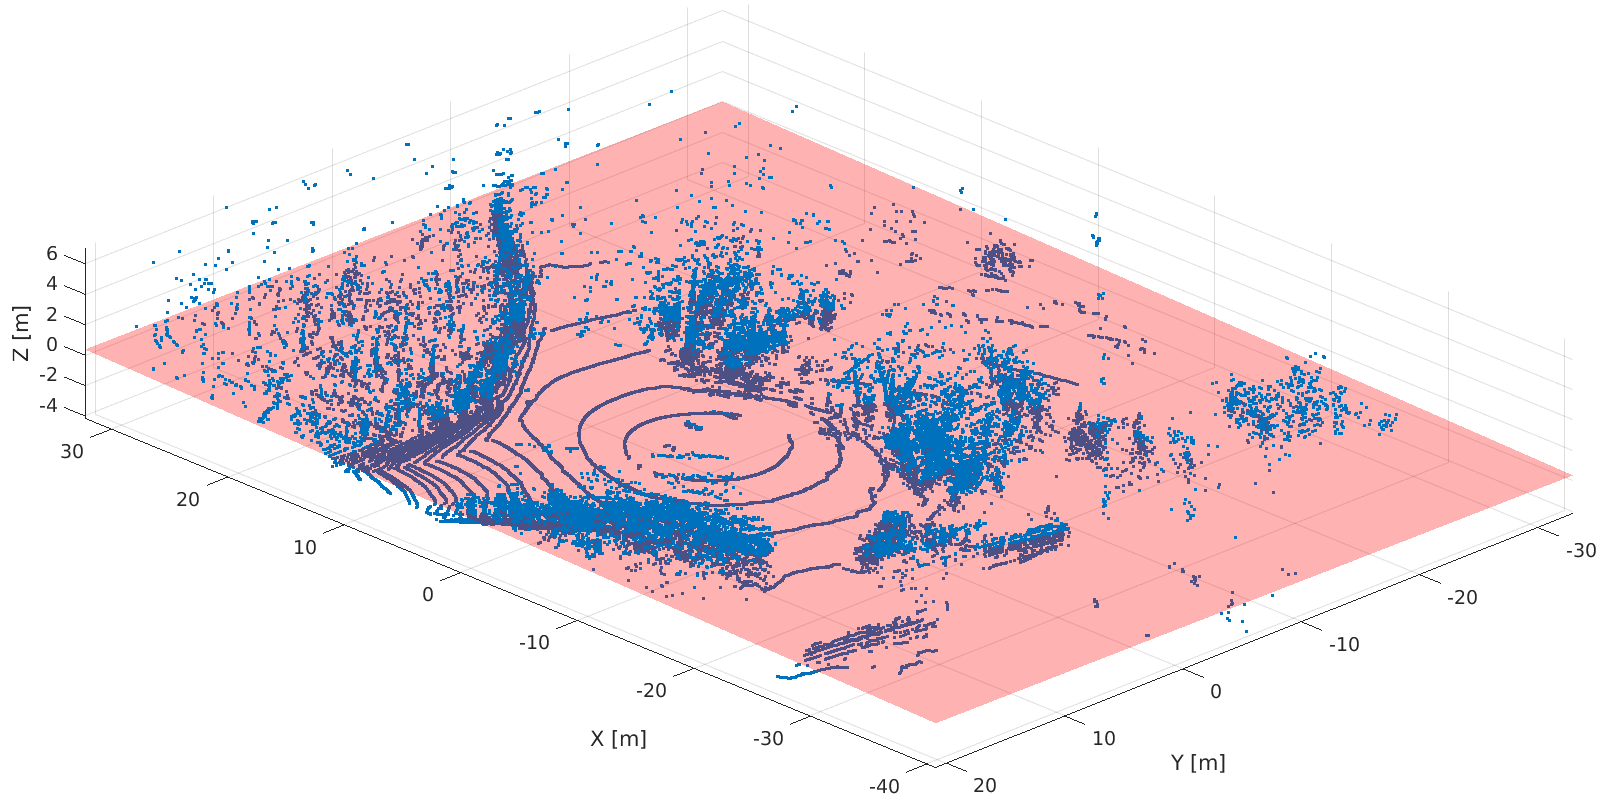
\includegraphics[width=0.7\linewidth]{Defense_Images/Method_Least_Squares_Plane_Proj.png}
			\caption[Method of Least Squares Plane Projection Example]{Method of Least Squares was used to project a plane unto point cloud data.}
			\label{fig:Method_Least_Squares_Plane_Proj}
		\end{figure}
		
	} % End Method of Least Squares Planar Fit
	
	\section{Random Sample Consensus (RANSAC)}{
	
		{RANSAC is an iterative algorithm that is designed to handle large numbers of outliers in the sample data set \cite{derpanis_overview_nodate,yaniv_random_2010,fischler_random_1987,cantzler_random_nodate}, and may be used to fit a two dimensional plane unto a three dimensional point cloud. RANSAC may be described as a two step process that may be repeated until a desired level of accuracy is achieved. Randomly selected samples from the data set are fitted with a model and the corresponding model parameters are determined. Number of samples corresponds to the desired model, therefore three points will be selected for plane fitting. Next the entire data set is examined with a cost function to determine consistency with the model. Number of points within the model or inliers is a common method of determining the best estimate \cite{cantzler_random_nodate}. A simplified two dimensional example is shown in Figure \ref{fig:Ransac_2D_Example}. RANSAC model parameters are not generally precise in order to decrease computational load, therefore necessitating a secondary algorithm to analyze a subset of the point cloud. Method of least squares is one such algorithm commonly employed for determining the best fit for the model.}

		\begin{figure}[H]
			\centering
			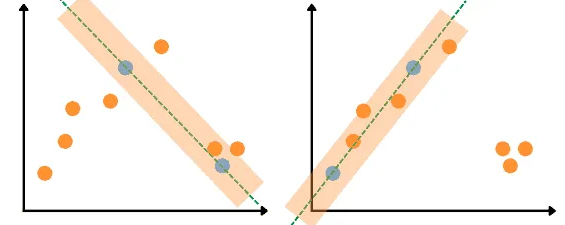
\includegraphics[width=0.7\linewidth]{Defense_Images/RANSAC_good_and_bad.png}
			\caption[2D Simplified RANSAC Example]{Line fitment on a 2d set of points using RANSAC \cite{alam_using_2022}. Poor fitment (left) is shown with minimal number of points within the user-defined threshold area. Better fitment (right) is shown with maximum number of points within the user-defined threshold area.}
			\label{fig:Ransac_2D_Example}
		\end{figure}

		{While RANSAC provides a robust estimation for model parameters, the primary disadvantage is potentially high computationally load \cite{yaniv_random_2010} however as reference planes in this work were projected on small data sets, alleviating computational load. Restricting the number of iterations decreased the likelihood of having the best fit while decreasing the computation time.}
	
%		{ was able to project a plane unto point cloud data gathered from the VLP-32C LiDAR (Figure \ref{fig:RANSAC_example_proj}).}
		
		\begin{figure}[H]
			\centering
			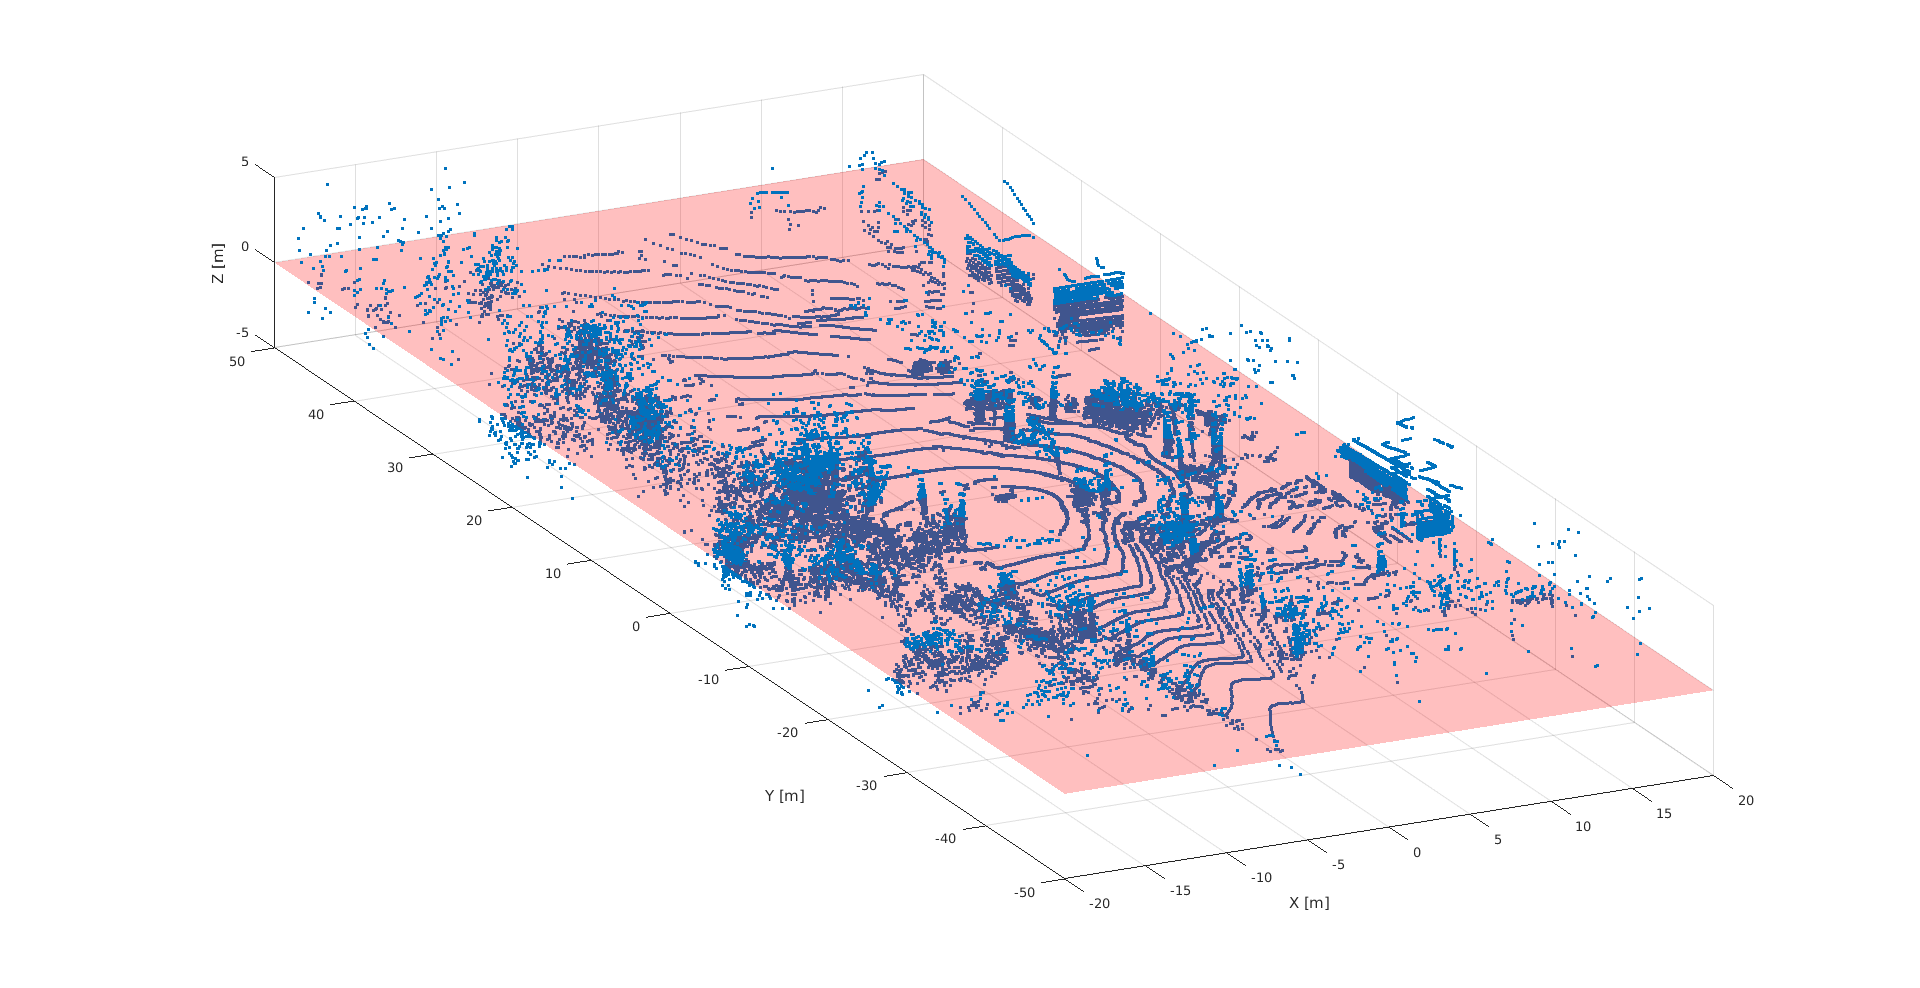
\includegraphics[width=0.7\linewidth]{Defense_Images/RANSAC_example_proj.png}
			\caption[RANSAC Plane Projection Example]{RANSAC plane projection over a point cloud gathered from the VLP-32C Scanning LiDAR using MATLAB's $pcfitplane$.}
			\label{fig:RANSAC_example_proj}
		\end{figure}
		
	} % End RANSAC
	
	\section{Random Decision Forests (RDF)}\label{RDF_SECT}{
		
		{Random Decision Forests is a supervised machine learning method that operates on a set of decision trees \cite{ho_random_1995}. Random Decision Forests have been shown to be useful with handling LiDAR data sets \cite{breiman_random_2001}, and have been employed in terrain classification \cite{laible_3d_2012,laible_map_building,laible_terrain_2013,khan_high_2011,reymann_improving_2015,schilling_geometric_2017, wietrzykowski_context-aware_2019}. Multiple decision trees are created with bootstrapped data sets - randomly selected data sub-sets from a training set. Classification may be determined by the majority results as opposed to the mean \cite{breiman_random_2001,ho_random_1995}. Random Decision Forests may be used to predict road surface area by detecting gravel terrain. Three data bases are conventionally used to train and develop a machine learning algorithm: Training, Testing, and Verification. Training data is the data set from which the Random Decision Forest trains. Training data sets must have roughly equal number of each class to avoid over-training. Training with uneven amounts of data per class type tends to over-classify data as the majority class. Sufficiently large training data sets are necessary to avoid over-training the algorithm to the training data set. Training with a smaller training data set tends to train the algorithm to miss-classify data that does not precisely match the training data set. Testing data is a data set that is independent of the training data but is roughly similar to the training data set. Random Decision Forests do not require a testing data set, as training data is bootstrapped from a larger data set and training data that is not selected may be used as the testing data set. Verification or validation data sets are used to provide an unbiased evaluation of the model by providing data that is non-negligibly dissimilar to the training to testing data sets. } 
		
		{MATLAB's Classification Learner Application may be used to generate a Random Decision Forests for each considered scanning LiDAR channel. Decision tree depth, number of learners, and number of features to consider for each binary split are hyper-parameters that may be optimized using MATLAB's Bayesian Optimization.}
	
	} % End RDF

	\subsection{Bayesian Optimization}\label{Bayesian_Optimization}{
		
		{Bayesian Optimization may be used to tune the hyper parameters of a machine algorithm \cite{noauthor_bayesian_nodate, snoek_practical_2012}. Bayesian Optimization initializes a surrogate function to represent the objective function (in this case minimum total classification error) with randomly selected hyper-parameters. Additional points on the objective function are chosen using an acquisition function to determine the utility of potential hyper-parameters. Best predicted hyper-parameters are used to retrain the Random Decision Forest. Objective function results are used to update the surrogate function. Process is repeated until a specified number of runs.}
		
	} % End Bayesian
	
	\section{Closing Statements on Related Work}{
		
		{Current road detection models principally rely upon preexisting geometric or visible features. Localization may be completed by comparing a point cloud of a vehicle's local area to a previously built map of the area using Iterative Closest Point. Neither method may suffice for rural environments, where generalized road features do not exist or the creation of maps would be considered impracticable due to storage constraints. LiDAR has been shown to perform successful terrain classification, and may be able to determine road surface area. Regression analysis may be completed with Method of Least-Squares or a RANSAC based method in order to project a plane unto a point cloud, which will serve as a baseline for examining point cloud spatial properties. Random Decision Forest Classification is an established method for LiDAR-based terrain classification using machine learning.}
		
	} % End Closing Statements
	
} % End Literature Review

\chapter{Methodology}{
	
	\section{Overview}
		
		\begin{figure}[H]
			\centering
			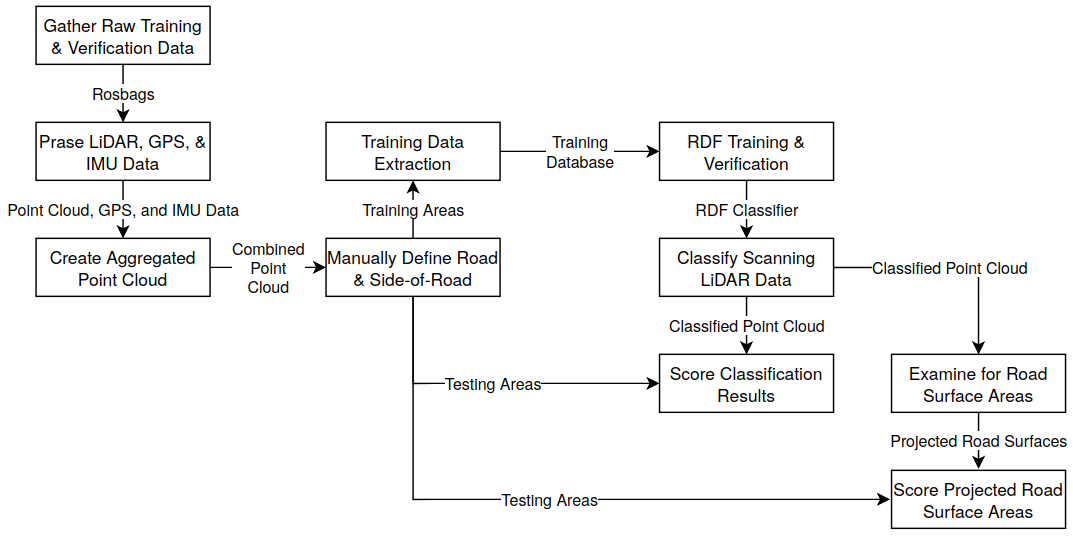
\includegraphics[width=0.9\linewidth]{Defense_Images/flowz_7}
			\caption[Project Flow]{Flowchart describing the high-level process of this work.}
			\label{fig:flowz_7}
		\end{figure}
		
		{Detection of unmarked gravel road surfaces using terrain classification requires building a data base of terrain features, training an RDF, and testing the algorithm for accuracy of unmarked road detection (outline of work in Figure \ref{fig:flowz_7}). Raw data was gathered using the experimental apparatus, which has a Velodyne VLP-32C scanning LiDAR sensor, Novatel PwrPak 7D-E2 GNSS and INS system, and Mako cameras \textit{[Gather Training \& Testing Data]} (Section \ref{sec:experimental-apparatus-setup}). Robotic Operating System (ROS) was used to package incoming scanning LiDAR, GNSS, IMU, and camera sensor data as rosbags, which were unpacked using MATLAB tools to separate data streams \textit{[Extract LiDAR, GPS, and IMU Data]}. Prior to creating a training database, manual dictation of gravel and asphalt areas of the gathered point cloud data is necessary for automatic training data extraction. In order to do so, all scanning LiDAR data from a rosbag was aggregated in order to create a single point cloud map \textit{[Point Cloud]} (Section \ref{sec:aggregating_point_cloud_data}). Scanning LiDAR timestamps were matched to the closest GNSS and IMU timestamp data. Closest matching GNSS and IMU data informed the location and orientation of the LiDAR scan. Compiled point cloud maps were examined and compared to camera and satellite data to determine gravel and asphalt surface location. Manually defined 2D areas representing gravel and asphalt were projected unto the point cloud \textit{[Manually Define Road \& Side-of-Road]} (Section \ref{sec:training_and_verification_data_selection_process}).}

		{Training data was extracted from a single arc from each 360 degree LiDAR scan if the arc was coincident to a manually projected 2D area (Figure \ref{fig:test_vs_train_areas}). Raw spatial and intensity values from the coincident arc were saved to a raw training database \textit{[Training Data Extraction]}. Separate training data bases were maintained for each individual channel. Features that describe the raw spatial and intensity data were extracted. Thirty percent of the training data base was randomly selected and set aside as a validation data base. Training data was visually examined for clustering to verify that a Random Decision Forest would be able to be trained (Section \ref{sec:Feat_Extract}). It was found that each class generally clustered to a certain range with some overlap, which indicates that a Random Decision Forest may be trained. MATLAB was used to train a Random Decision Forests for each of the three considered channels using Bayesian Optimization to tune tree depth and number of splits \textit{[RDF Training \& Verification]} (Section \ref{sec:random-decision-forest-creation}). Training continued until a minimum error was reached. Validation of the RDF was then completed using the validation database (Section \ref{sec:random-decision-forest-verification}).}
		
		{Scanning LiDAR data from five datasets representing five drives on a stretch of Blackburn Road were classified \textit{[Classify Scanning LiDAR Data]}. Three arcs from three channels were considered for classification - the centers of the arcs were directly in front of the vehicle, and 45 degrees left and right of center, creating nine total areas in a 3x3 grid in front of the van (see Figure \ref{fig:area_example}). Following the same process as aggregating point clouds, GNSS and IMU data informed the location and orientation of the arcs in each 360 degree scan. All arcs were then classified as "asphalt", "gravel", or "unknown", and the averaged coordinates of each arc was aggregated into a single, classified point cloud (Figure \ref{fig:raw_classification_results}).}
		
		{Manually defined gravel, asphalt, and side-of-road areas were projected onto the classified point cloud and used to determine the accuracy of the terrain classification algorithm by determining the distribution of classified arcs per area \textit{[Score Classification Results]} (Section \ref{sec:consecutive_point_cloud_classification_scoring}). Classified point clouds were examined for trends across arcs to determine if the location of gravel and asphalt surfaces may be identified visually and automatically \textit{[Examine for Road Surface Areas]} (Section \ref{sec:manual_road_detection}). Guessed road surface areas were then compared to actual areas to determine the method's ability at unmarked gravel road discovery, indicating the method's efficiency at detecting intercepting gravel roads \textit{[Score Projected Road Surface Areas]}.}

	\section{Experimental Apparatus Setup}\label{sec:experimental-apparatus-setup}{
		
		{Required physical data was gathered by the Hexegon Chrysler Pacifica New Eagle DBW van (Figure \ref{fig:Experimental_Apperatus}), built by AutonomouStuff, owned and operated by Ohio University. LiDAR point cloud data was gathered with the vehicle's roof-mounted Velodyne VLP-32C. Velodnyne's VLP-32C has 32 channels producing 300,000 points per second with a vertical field of view from -45$^{\circ}$ to $+$15$^{\circ}$, providing a minimum 0.33$^{\circ}$ vertical angular resolution and 0.2$^{\circ}$ horizontal angular resolution \cite{vlp_32c}. Image data was captured with the forward facing Allied Vision Mako G-319C Cameras equipped with 16 and 12 mm lenses (Figure \ref{fig:makocamera}) producing 2064x1544 px resolution images at 37 Hz. GPS data was recorded by the van's PwrPak7D-E2 GNSS \& INS enclosure manufactured by Novatel equipped with two GNSS-502 antennas manufactured by NavtechGPS.}
		
		\begin{figure}[H]
			\centering
			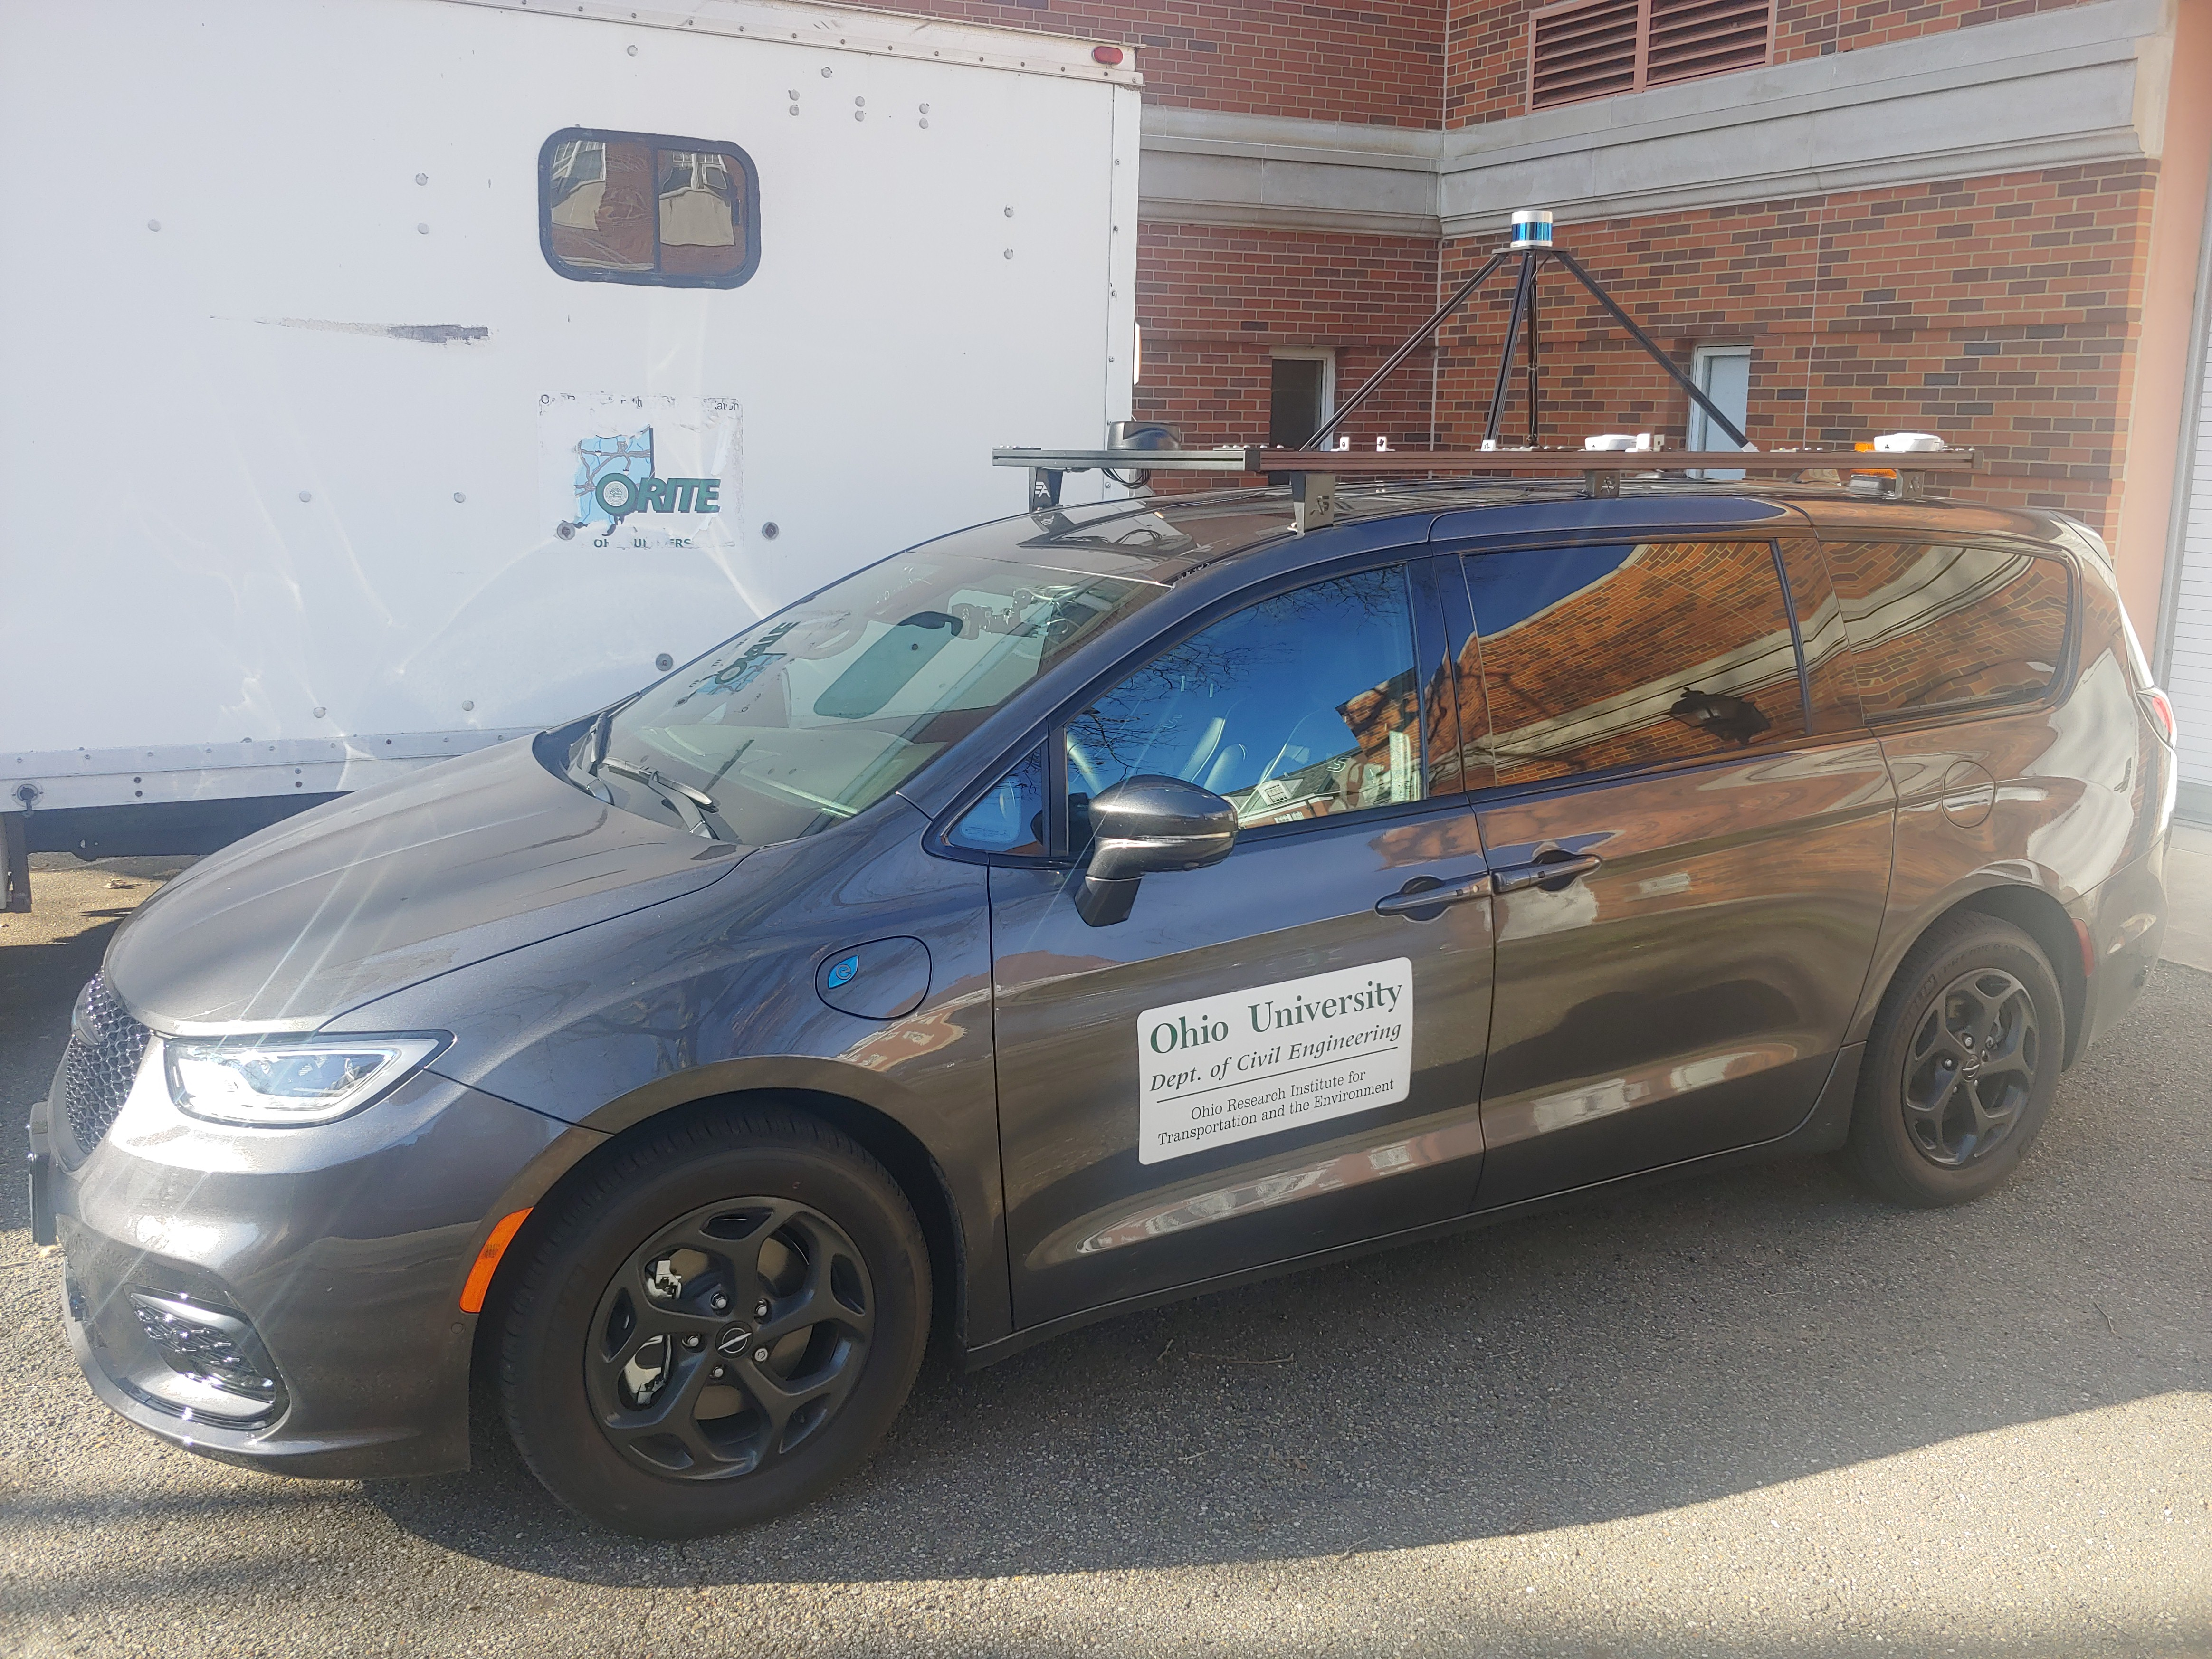
\includegraphics[width=0.7\linewidth]{Defense_Images/van_on_van}
			\caption[Sensor Van]{Sensor Van built by AutonomouStuff}
			\label{fig:Experimental_Apperatus}
		\end{figure}
	
		\begin{figure}[H]
			\centering
			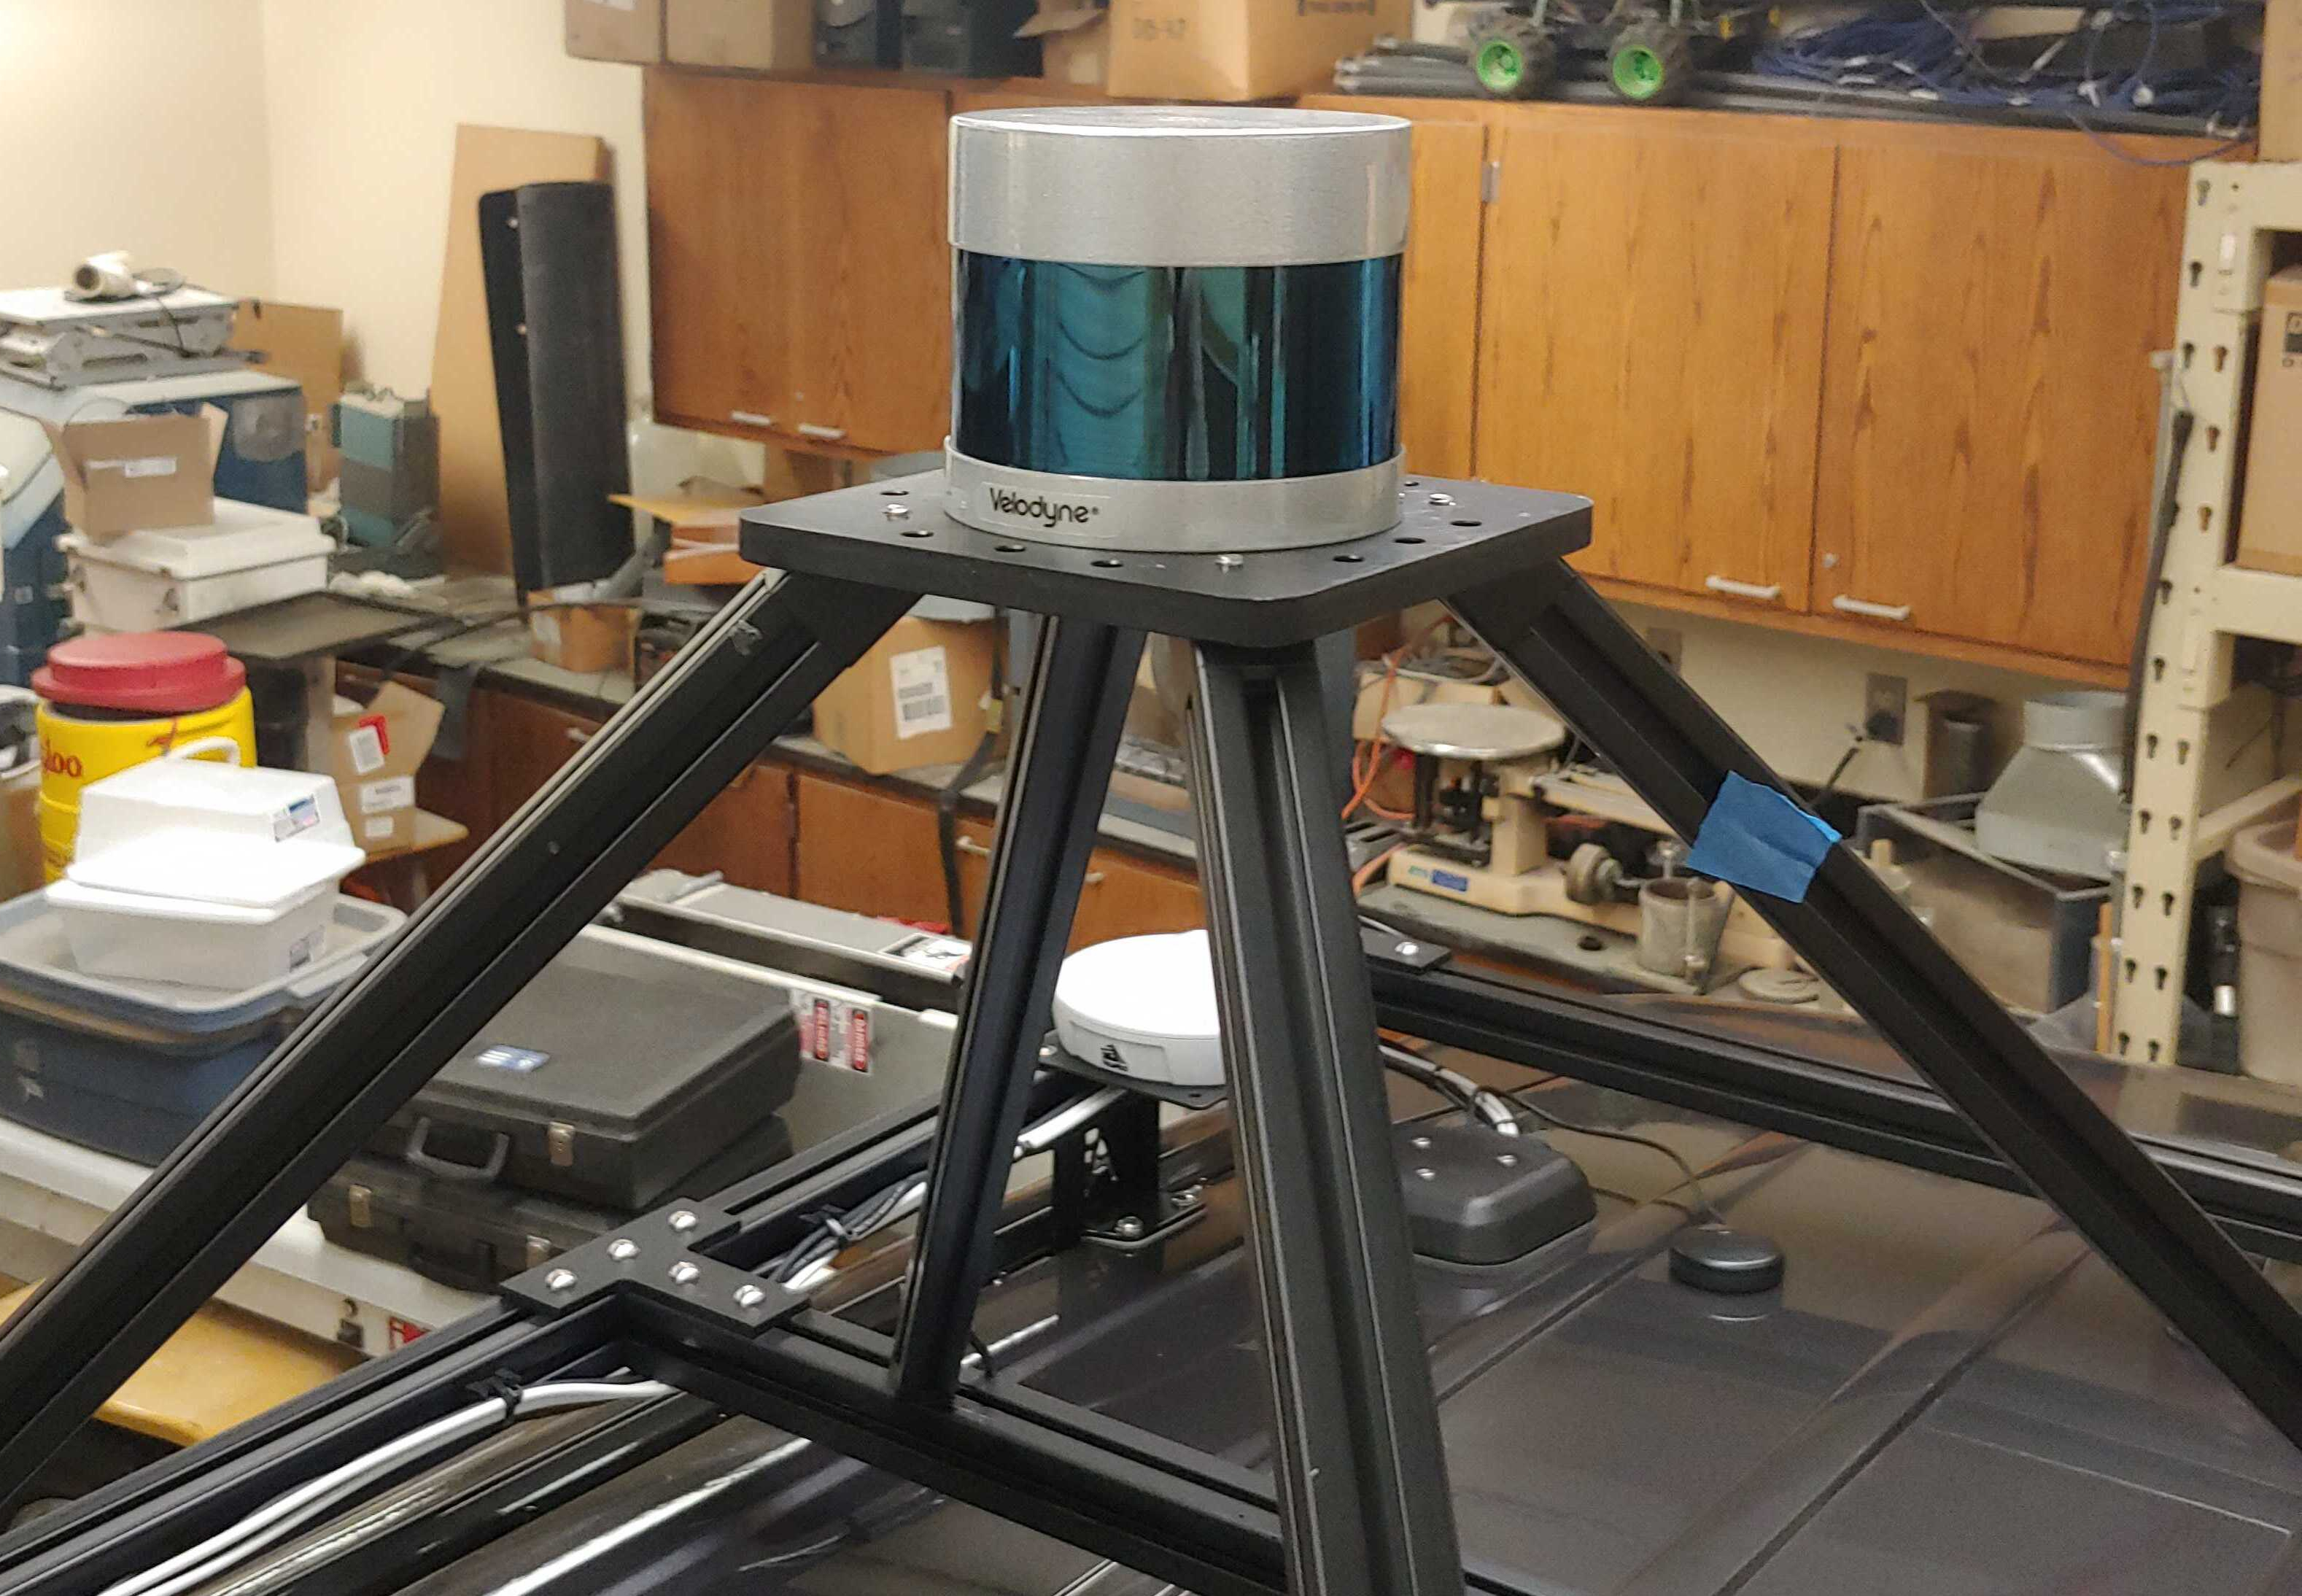
\includegraphics[width=0.7\linewidth]{Defense_Images/vlp_32_mount_2}
			\caption[VLP 32 on Van]{Velodyne's VLP-32 is mounted on top of the Sensor Van.}
			\label{fig:vlp32mount}
		\end{figure}
		
		\begin{figure}[H]
			\centering
			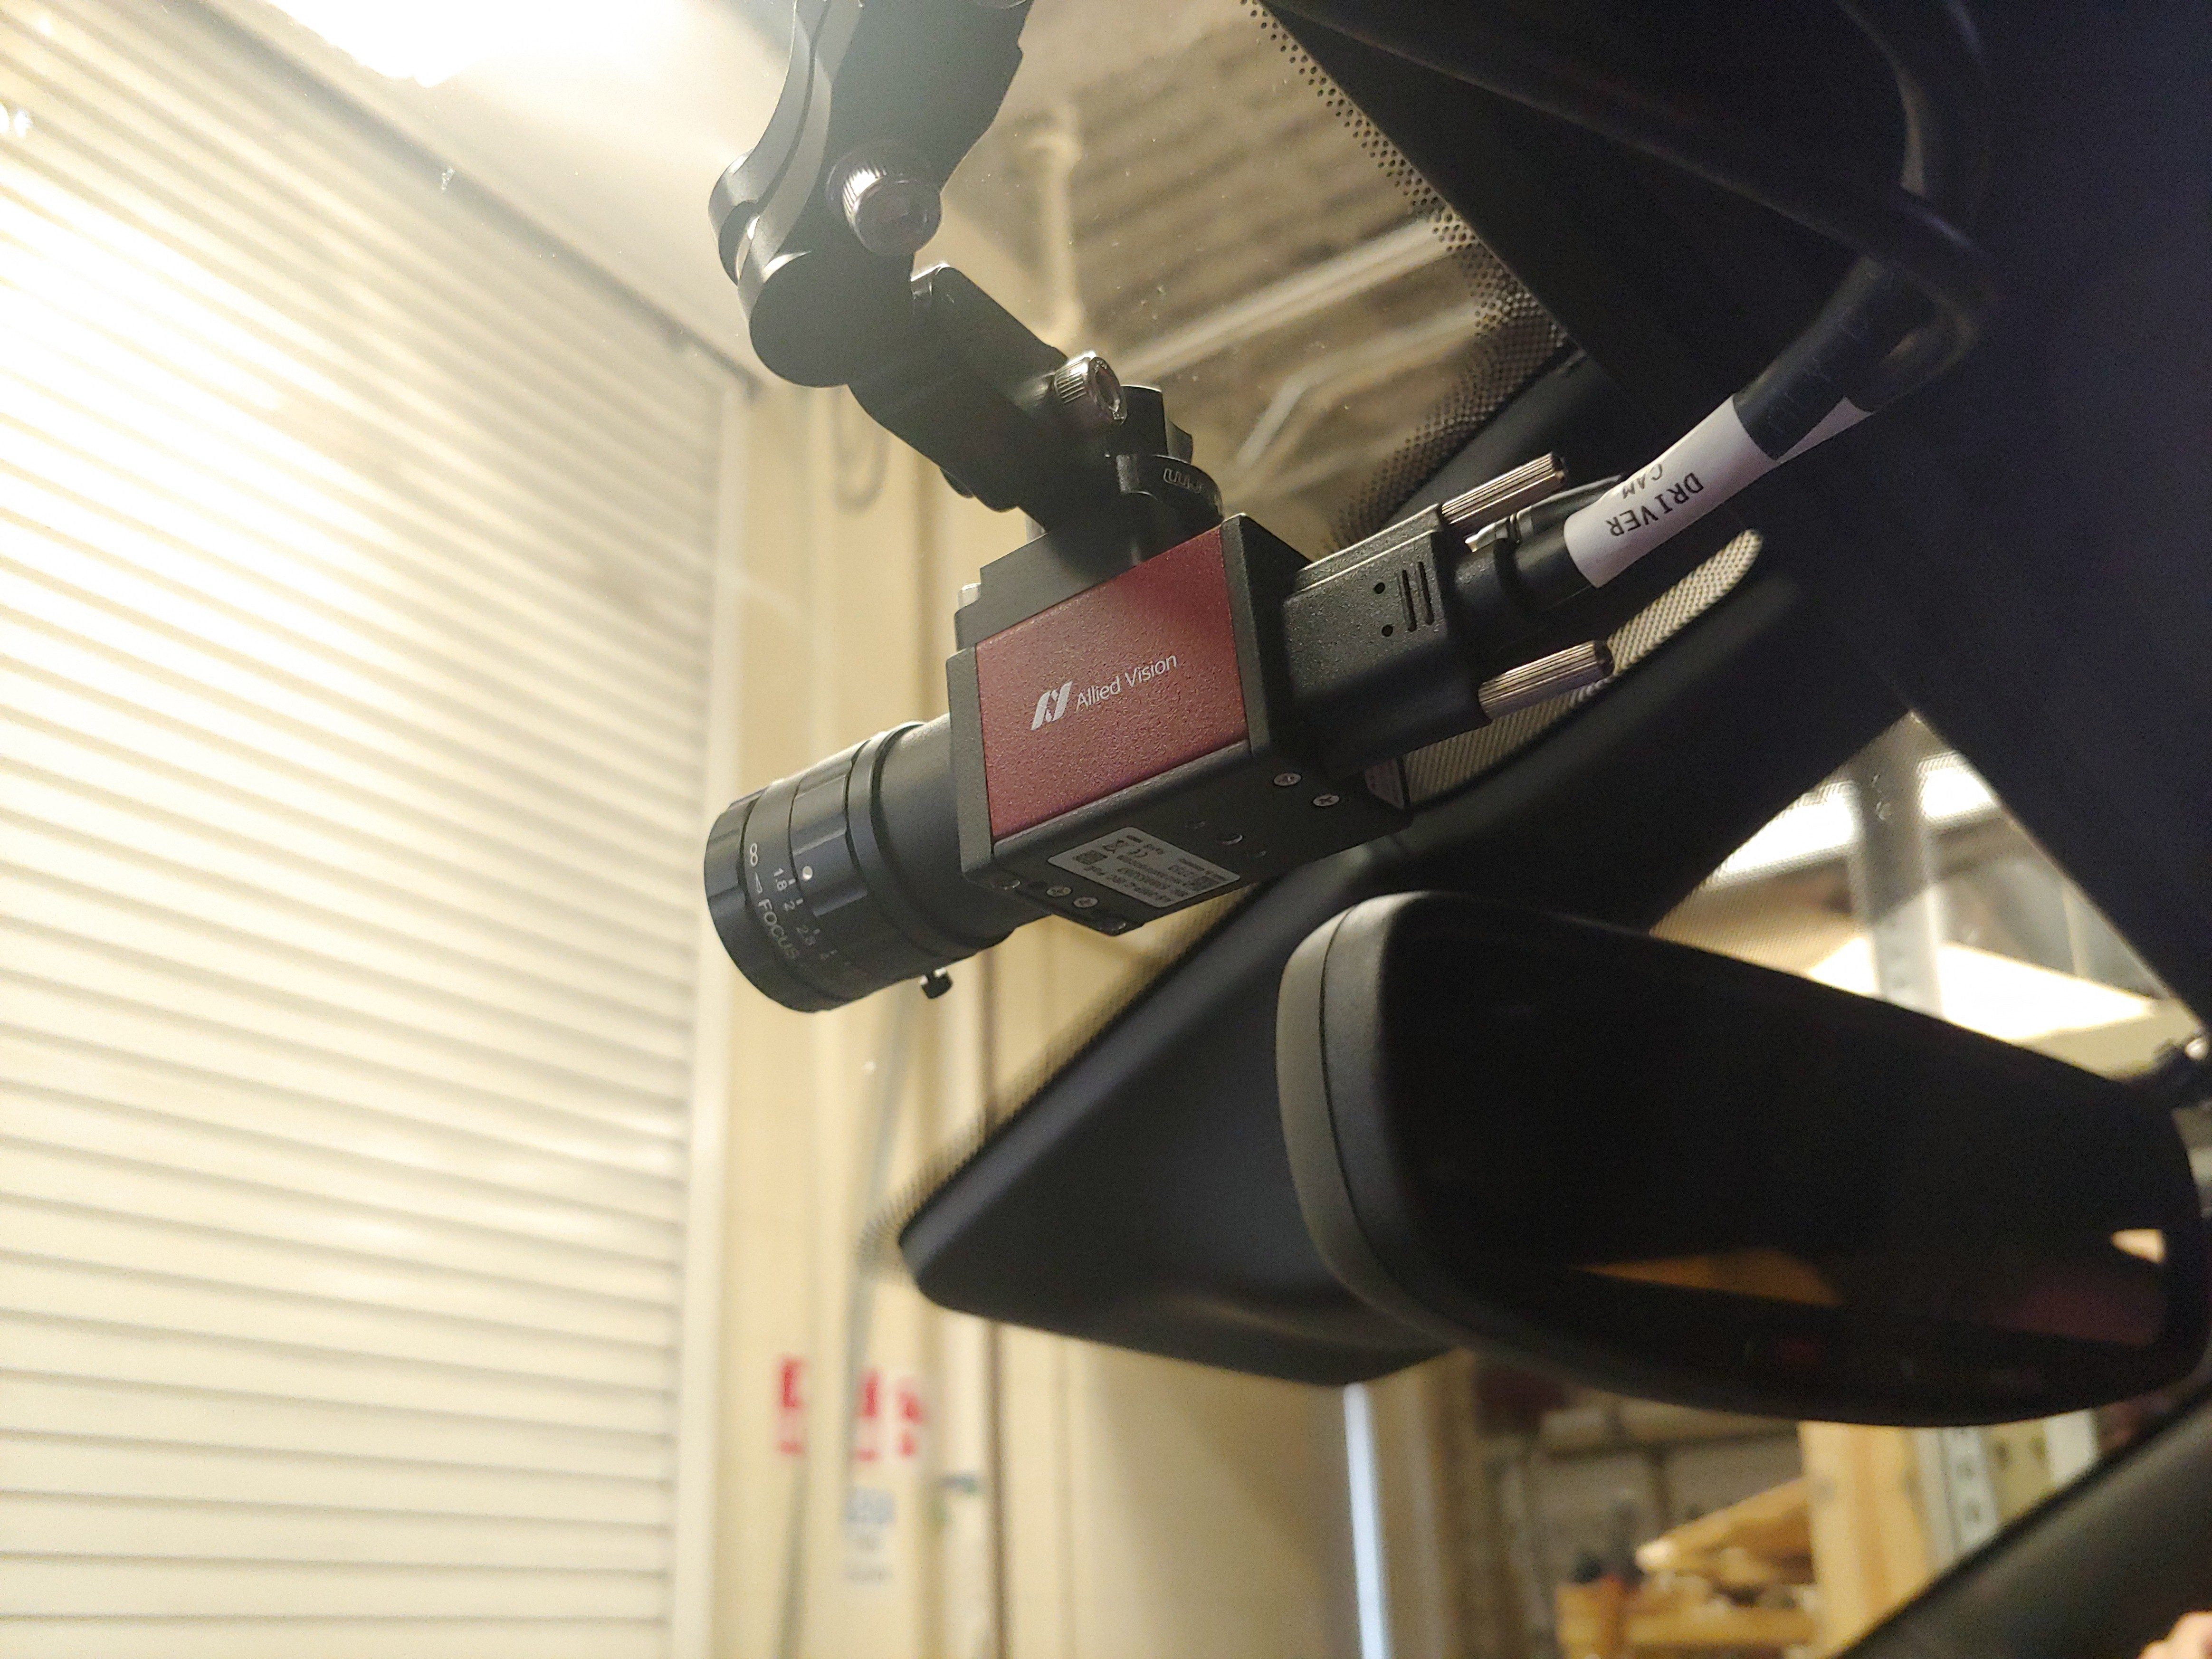
\includegraphics[width=0.7\linewidth]{Defense_Images/Mako_Camera}
			\caption[Mako Camera]{One of the two forward facing Mako Cameras in the van.}
			\label{fig:makocamera}
		\end{figure}
	
	} % Experimental Apparatus Setup
	
	\section{Data Collection}{
		
		{Scanning LiDAR data of a gravel surface was gathered from a gravel parking lot that intersects Blackburn Road near Athens Ohio (Figure \ref{fig:gravel_training_lot}). Including the lot from which gravel training data was gathered, three gravel driveways intersect Blackburn Road (Figure \ref{fig:three_driveways_sat}). Scanning LiDAR data of an asphalt surface was gathered from Blackburn Road near the intersecting gravel lot (Figure \ref{fig:Blackburn_Road_View}). Scanning LiDAR data of grassy surfaces was gathered next to the gravel lot. Although this work does not evaluate the detection accuracy of grass, differentiation between a road and non-road surface is necessary for evaluating road-surface detection, therefore grass is labeled as "unknown" in this work. Raw data was gathered using the Robotic Operating System (ROS) to package incoming scanning LiDAR, GNSS, IMU, and camera sensor data as rosbags.}
		
		%[width=1.0\linewidth,height=8.0 cm,keepaspectratio]
		\begin{figure}[H]
			\centering
			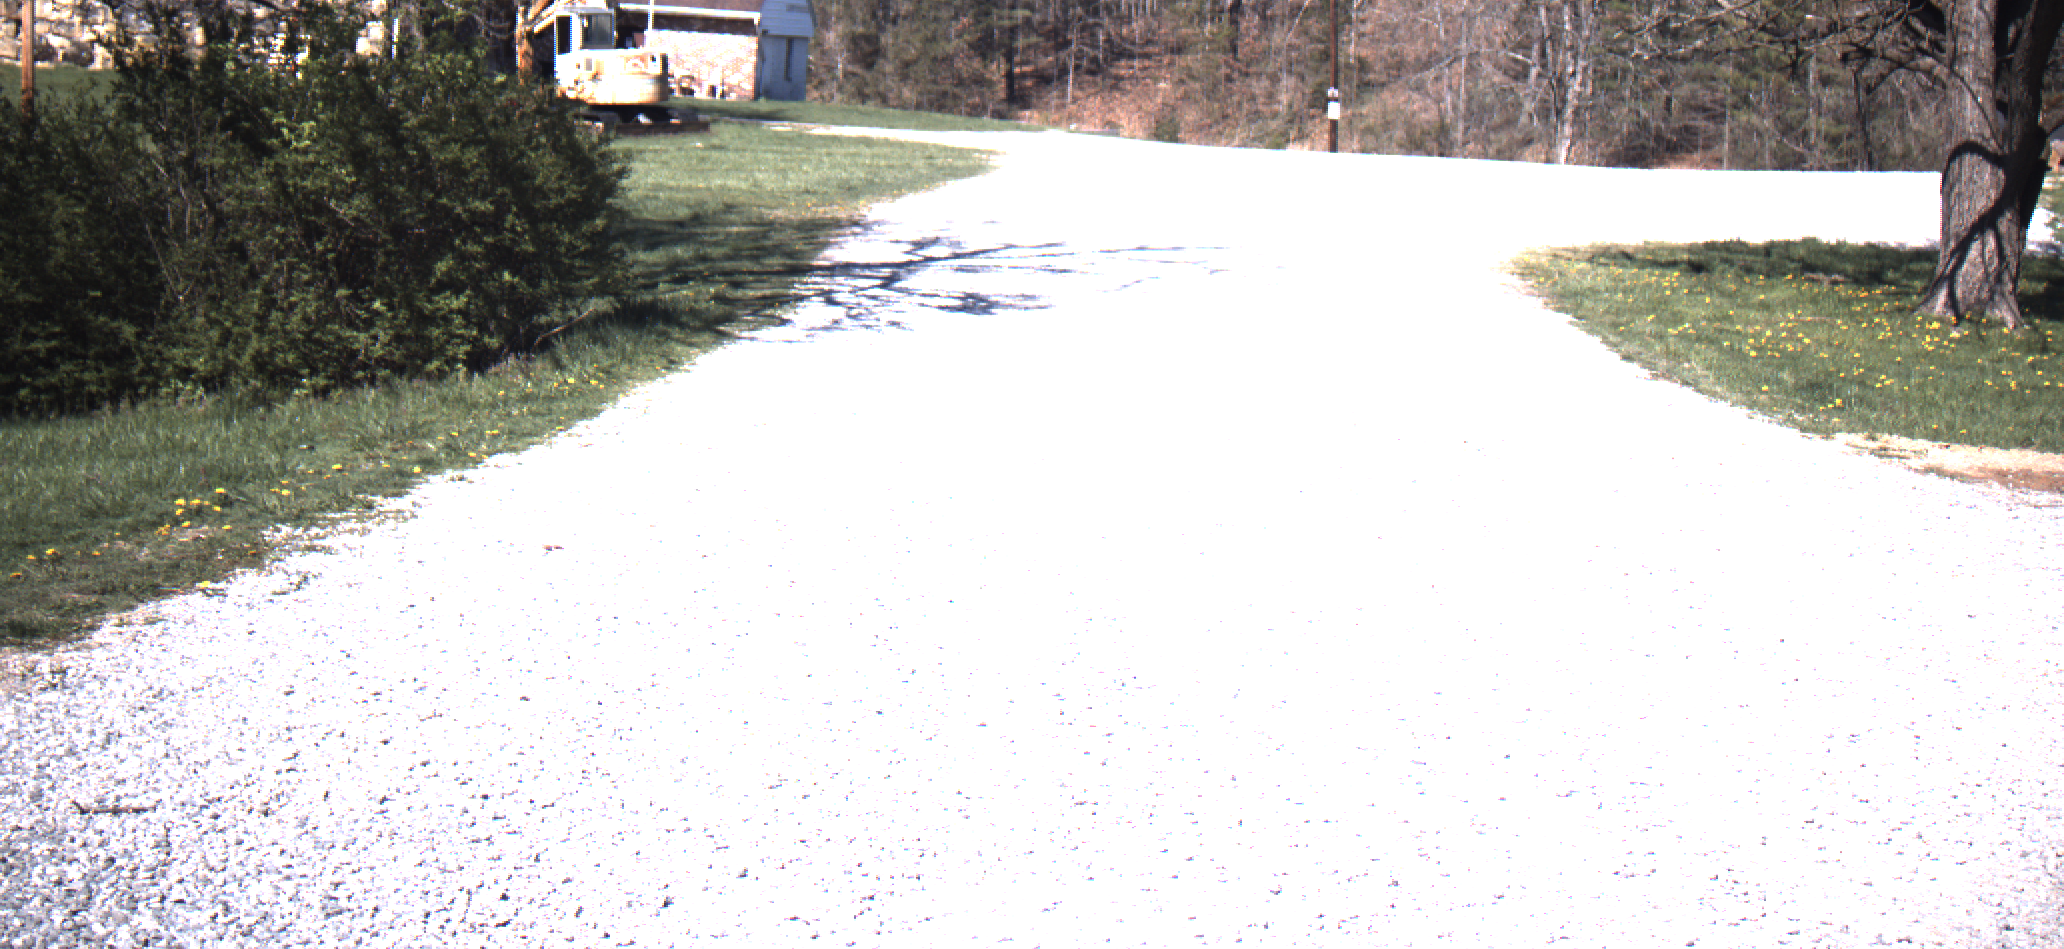
\includegraphics[width=0.75\linewidth]{Defense_Images/gravel_training_lot}
			\caption[Gravel Training Lot]{Camera view of the gravel lot from which gravel training data was gathered.}
			\label{fig:gravel_training_lot}
		\end{figure}
		
		\begin{figure}[H]
			\centering
			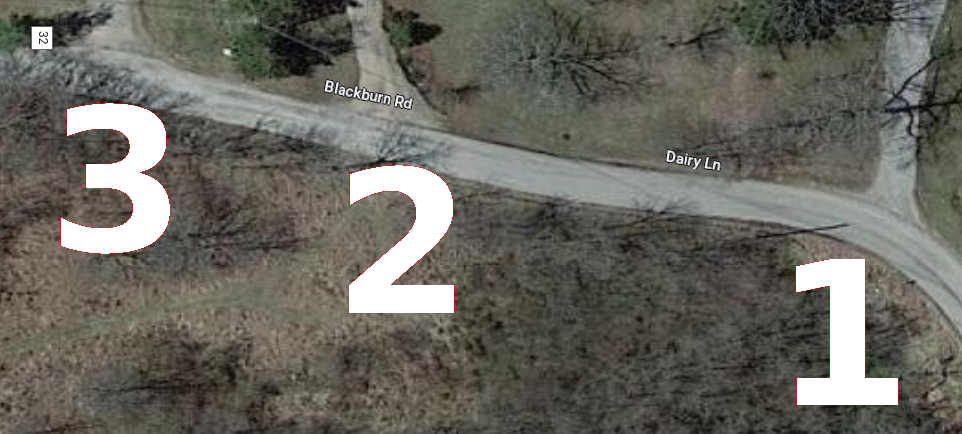
\includegraphics[width=0.75\linewidth]{Defense_Images/three_driveways_sat}
			\caption[Satellite View of Blackburn Road]{Satellite view of Blackburn Road. Three gravel driveways intercept Blackburn Road. }
			\label{fig:three_driveways_sat}
		\end{figure}
		
		
		\begin{figure}[H]
			\centering
			\includegraphics[width=0.75\linewidth]{Defense_Images/vlcsnap-2023-04-20-08h48m17s447}
			\caption[Blackburn Road Camera View]{Camera view of Blackburn Road - an unmarked asphalt road with three intercepting gravel driveways from which asphalt data was gathered.}
			\label{fig:Blackburn_Road_View}
		\end{figure}
					
	} % End Data Collection
		
	\section{Data Processing}\label{sec:data_processing}{

		{MATLAB was used to process the gathered rosbag files using the MATLAB ROSBAG library. Point cloud, GPS, and IMU topics were defined, and point cloud Cartesian coordinates with corresponding intensities, longitude, latitude, altitude, roll, pitch, and yaw messages were read from the appropriate topics and imported.}

	} % End Data Processing
	
%		\section{Transformation Matrix Derivation} \label{sec:grab_tform} {
%			
%			{Point cloud translation and rotation was accomplished using transformation matrices that were derived from GPS and IMU data stored in a rosbag. GPS and IMU  time stamps that most closely matched LiDAR timestamps were found. Rotation matrices were created using extracted roll, pitch, and yaw data from the IMU. LiDAR origin was found using GPS longitude, latitude, and altitude data. Physical distances between the GPS, IMU, and LiDAR was rectitude by obtaining reference frames provided by AutonomouStuff (Section \ref{sec:experimental-apparatus-setup}). GPS coordinates were offset by the current orientation and converts the ground truth to the LiDAR frame. GPS, IMU, and LiDAR reference frames and rotational updates were combined into trajectory vectors. Transformation matrices were then derived using MATLAB's $rigid3d$ function. Consecutive point cloud scans may then translated and rotated with derived transformation matrices (Figure \ref{fig:Compiled_PCD}).}
%			
%		} % End Transformation Matrix Derivation
	
	\section{Aggregating Point Cloud Data}\label{sec:aggregating_point_cloud_data}{
	
		{Scanning LiDAR training data requires extraction from manually defined gravel, asphalt, and unknown terrain areas on aggregated point clouds as manual extraction from consecutive single scans is extremely time consuming. Aggregating LiDAR data into a single point cloud was completed by post processing rosbags that contained scanning LiDAR, GPS, and IMU data of an unmarked road. Scanning LiDAR timestamps were matched to the closest GNSS and IMU timestamp data. Closest matching GNSS and IMU data informed the location and orientation of the LiDAR scan. Point cloud translation and rotation was accomplished using transformation matrices derived from GPS and IMU data. Rotation matrices were created using extracted roll, pitch, and yaw data from the IMU. LiDAR origin was found using GPS longitude, latitude, and altitude data. Physical distances between the GPS, IMU, and LiDAR sensors was rectified by obtaining reference frames provided by AutonomouStuff. GPS coordinates were offset by the current orientation and converted the ground truth to the LiDAR frame. GPS, IMU, and LiDAR reference frames and rotational updates were combined into trajectory vectors. Transformation matrices were then derived using MATLAB's $rigid3d$ function. Consecutive point cloud scans may then translated and rotated with derived transformation matrices (Fig. \ref{fig:Compiled_PCD}). While not as robust as more sophisticated methods of point cloud aggregation such as NDT or ICP scan matching, over shorter distances using this method proved to be adequate for this work.} 
		
		\begin{figure}[H]
			\centering
			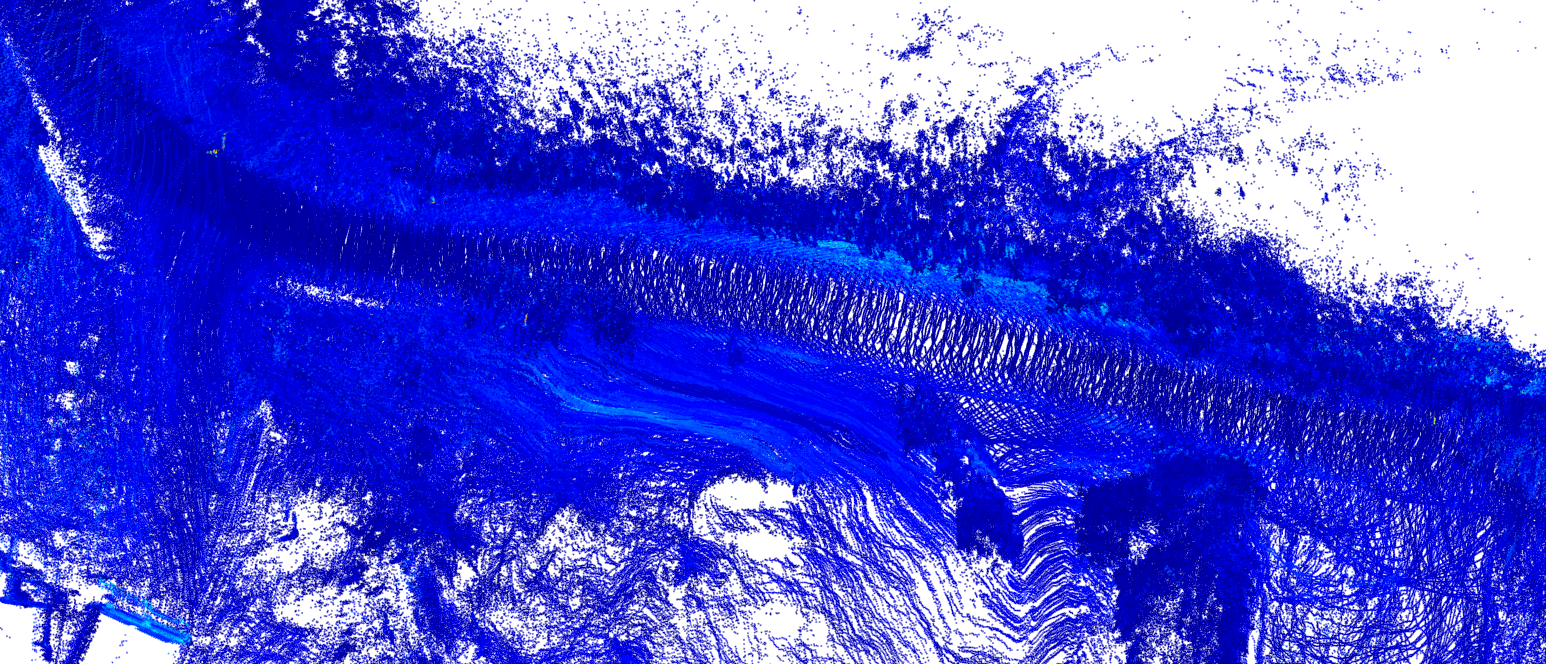
\includegraphics[width=0.9\linewidth]{Defense_Images/pc_example}
			\caption[Compiled Point Cloud Data]{Example compiled point cloud data}
			\label{fig:Compiled_PCD}
		\end{figure}
	
	} % Aggregating Point Cloud Data

	\section{Training and Verification Data Selection Process}\label{sec:training_and_verification_data_selection_process}{

		{Scanning LiDAR training data was gathered from rosbags containing scanning LiDAR, GPS, and IMU data in a two step process. Combined point cloud data was loaded into the MATLAB environment and displayed (Figure \ref{fig:pre_select_area}). Manually defined areas representing gravel, asphalt, or unknown were created and projected unto the combined point cloud. MATLAB's $drawpolygon$ function was used to select an area representing gravel, asphalt, or unknown (Figure \ref{fig:area_selected}). Areas were conservatively selected in order to ensure that the areas only would contain terrain that was only a single desired terrain type. }

		\begin{figure}[H]
			\centering
			\begin{subfigure}{0.45\textwidth}
				\centering
				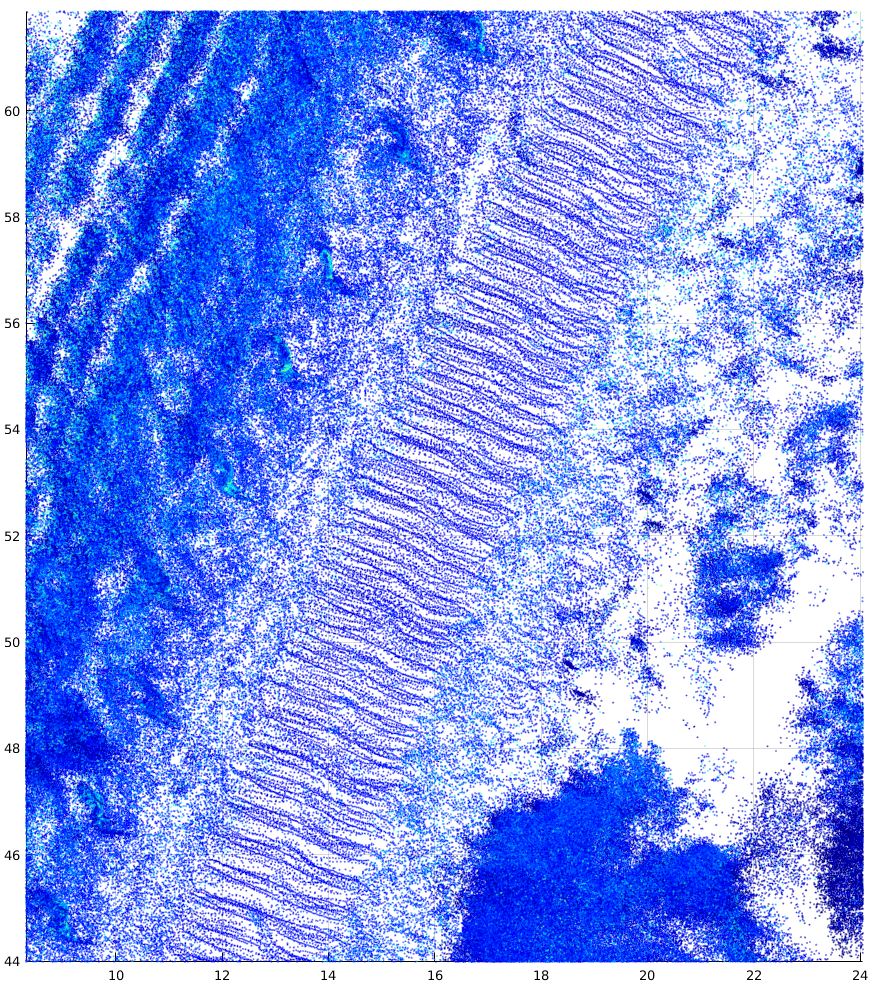
\includegraphics[width=1.0\linewidth]{Defense_Images/pre_select_area}
				\caption[Road area on Point Cloud]{}
				\label{fig:pre_select_area}
			\end{subfigure}
			\begin{subfigure}{0.45\textwidth}
				\centering
				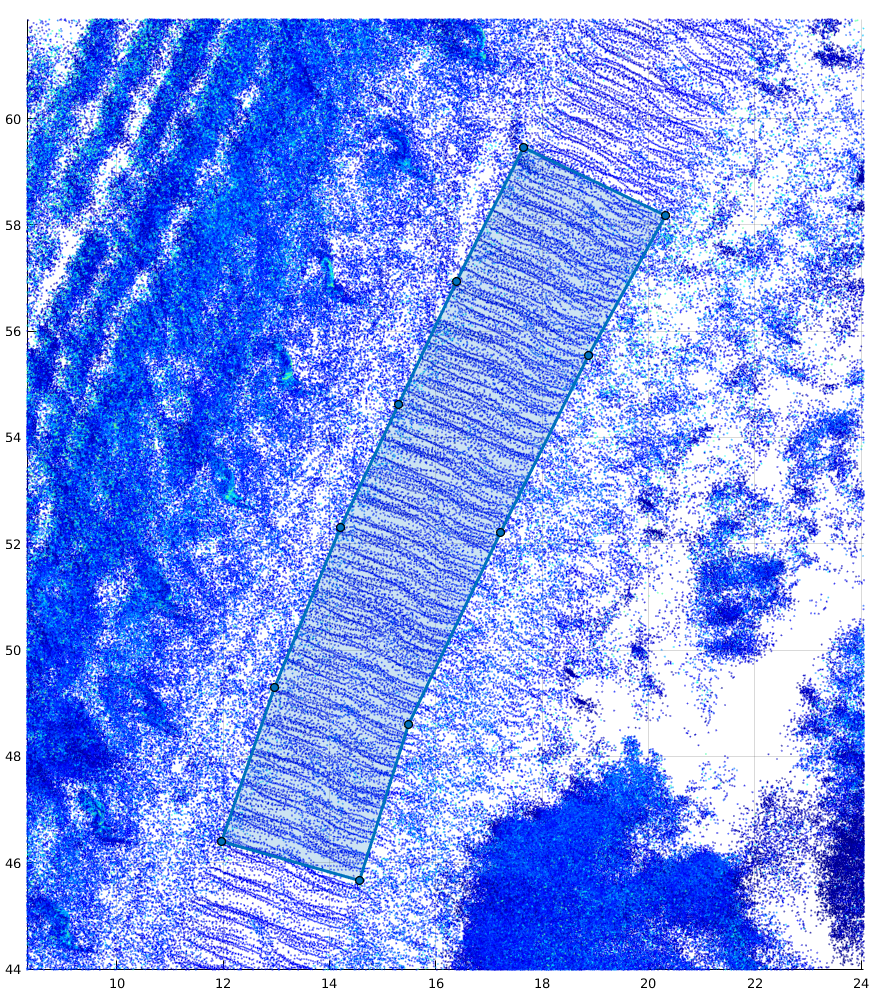
\includegraphics[width=1.0\linewidth]{Defense_Images/area_selected}
				\caption[Selected Road area on Point Cloud]{}
				\label{fig:area_selected}
			\end{subfigure}
			\caption[Manual Area Selection Process]{Combined scanning LiDAR point cloud data (a) may be manually defined using MATLAB's $drawpolygon$ function to select the desired area. }
			\label{fig:Area_Selection_Process}
		\end{figure}
	
		{Manually defined areas may then be overlayed unto the point cloud representing training areas (Fig. \ref{fig:test_vs_train_areas}) using MATLAB's $inpolygon$ function. Six degree arcs (Fig. \ref{fig:area_example}) from the first three channels of scanning LiDAR data that lay directly in front of the vehicle were extracted and exported to a database if coincident with the manually defined areas. Training data was extracted from a single arc from each 360 degree LiDAR scan if the arc was coincident to a manually projected 2D area. Raw spatial and intensity values from the coincident arc were saved to a raw training database. Separate training databases were maintained for each individual channel. Features that describe the raw spatial and intensity data were extracted. }
		
		\begin{figure}[H]
			\centering
			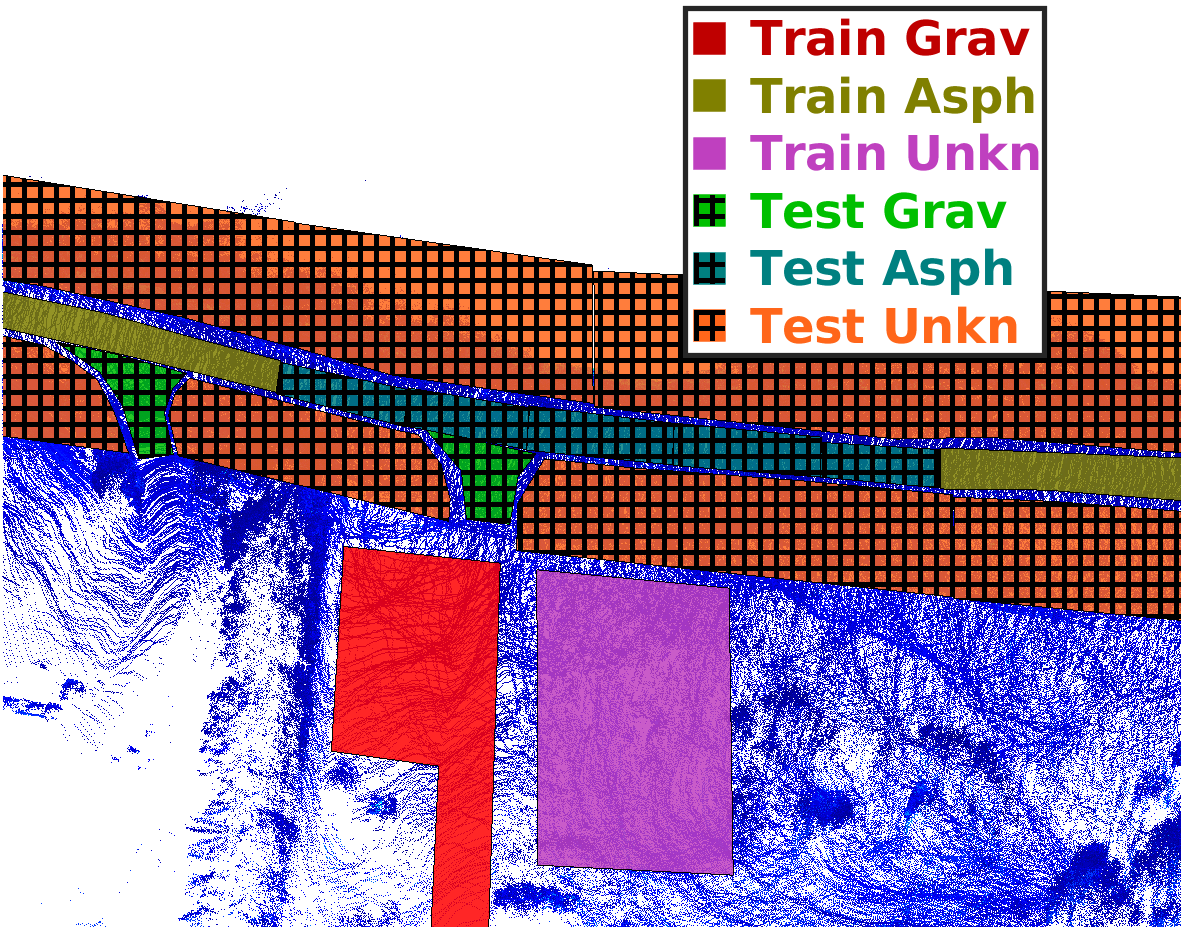
\includegraphics[width=0.95\linewidth]{Defense_Images/test_vs_train_areas_hatch}
			\caption[Training vs Testing Areas]{Training areas were kept separate from the testing areas.}
			\label{fig:test_vs_train_areas}
		\end{figure}
		
		\begin{figure}[H]
		\centering
		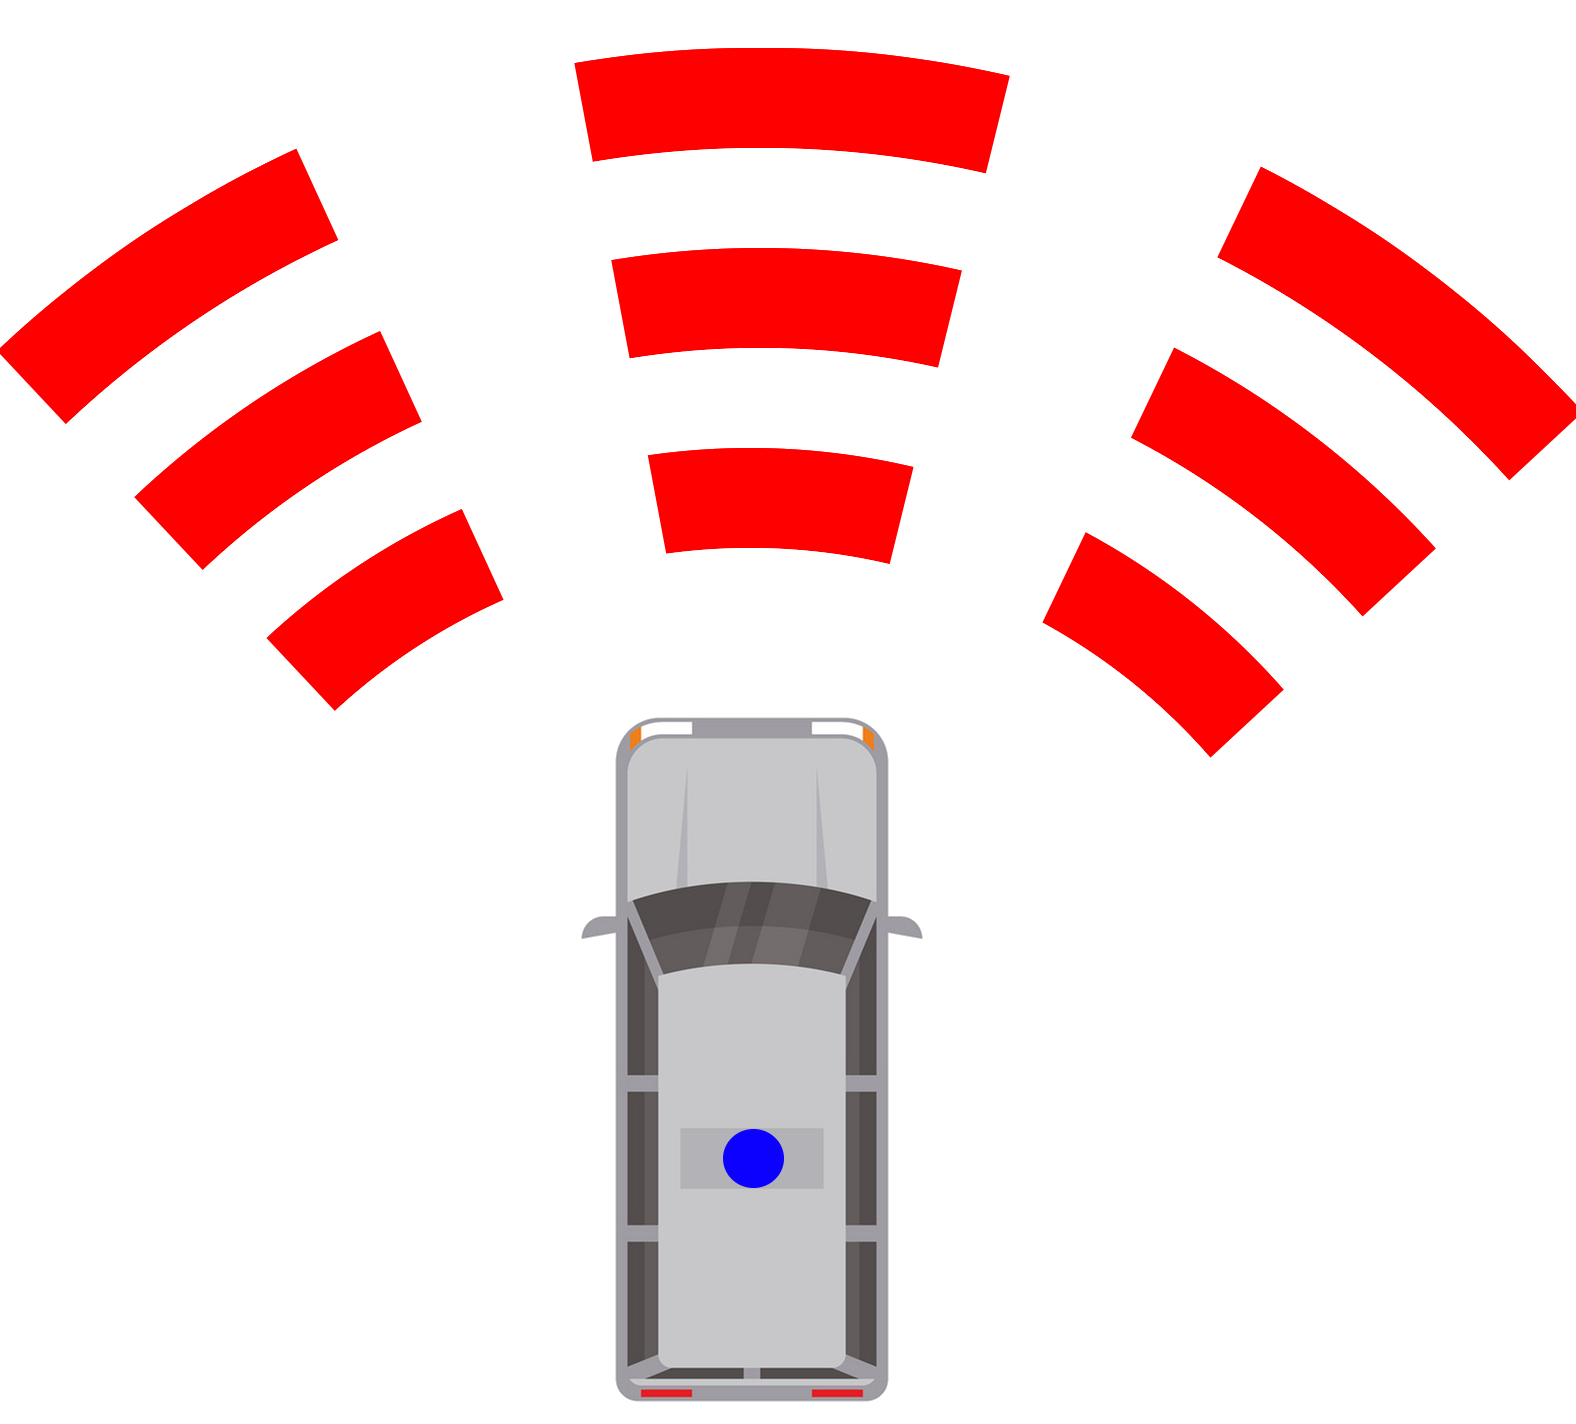
\includegraphics[width=0.25\linewidth]{Defense_Images/area_example}
		\caption[Areas to Classify]{Three arcs from three channels were classified per 360 degree scan. }
		\label{fig:area_example}
		\end{figure}
	
	} % End Training and Verification Data Selection Process
	
	\section{Feature Extraction}\label{sec:Feat_Extract} {
	
		{LiDAR returns spatial data represented by Cartesian coordinates with units in meters and remission data represented by a dimensionless ratio of minimum to maximum detected brightness. Feature extraction was completed by performing mathematical functions on the gathered spatial training data. This work examines three reference spatial reference points for spatial feature extraction \ref{fig:xy_vs_range}. \textbf{RANGE} refers to the algorithm that was trained using the LiDAR point of origin as the reference point. \textbf{RANSAC} and \textbf{MLS} refers to the algorithm that was trained using a RANSAC and MLS projected plane unto an arc as the spatial reference point respectively. Reference plane normal vector and distance from origin $[a,b,c,d]$ was derived from RANSAC and MLS methods for each arc segment. Per-point distance from the reference plane was calculated. Spatial features were non-dimensionalized as necessary by dividing by the average range of the arc to LiDAR point of origin to the appropriate power. As remission is a ratio of minimum to maximum (0 - 255) detectable reflected intensity there was no need to render the features non-dimensionalized. Thirty percent of the training data was randomly selected and reserved to create a validation data set. Features extracted include the following:}
		
		\begin{multicols}{2}
			\begin{itemize}[itemsep=.1pt]
				\item Standard Deviation
				\item Roughness
				\item Min Max Ratio
				\item Min Squared Max Ratio
				\item Gradient
				\item Mean (Remission Only)
			\end{itemize}
			\vfill\null
			\columnbreak
			\begin{itemize}[itemsep=.1pt]
				\item $std$
				\item $max - min$
				\item $min / max$
				\item $min^2 / max$
				\item $sqrt(sum(Gradient\*))$
				\item $mean$
			\end{itemize}
			\vfill\null
			\label{lst:feature_list}
		\end{multicols}
		
		{where $Gradient$ refers to the difference between consecutive numbers in an array. These features closely follow convention when describing scanning LiDAR data \cite{breiman_random_2001}.}
		
		
		\begin{figure}[H]
			\centering
			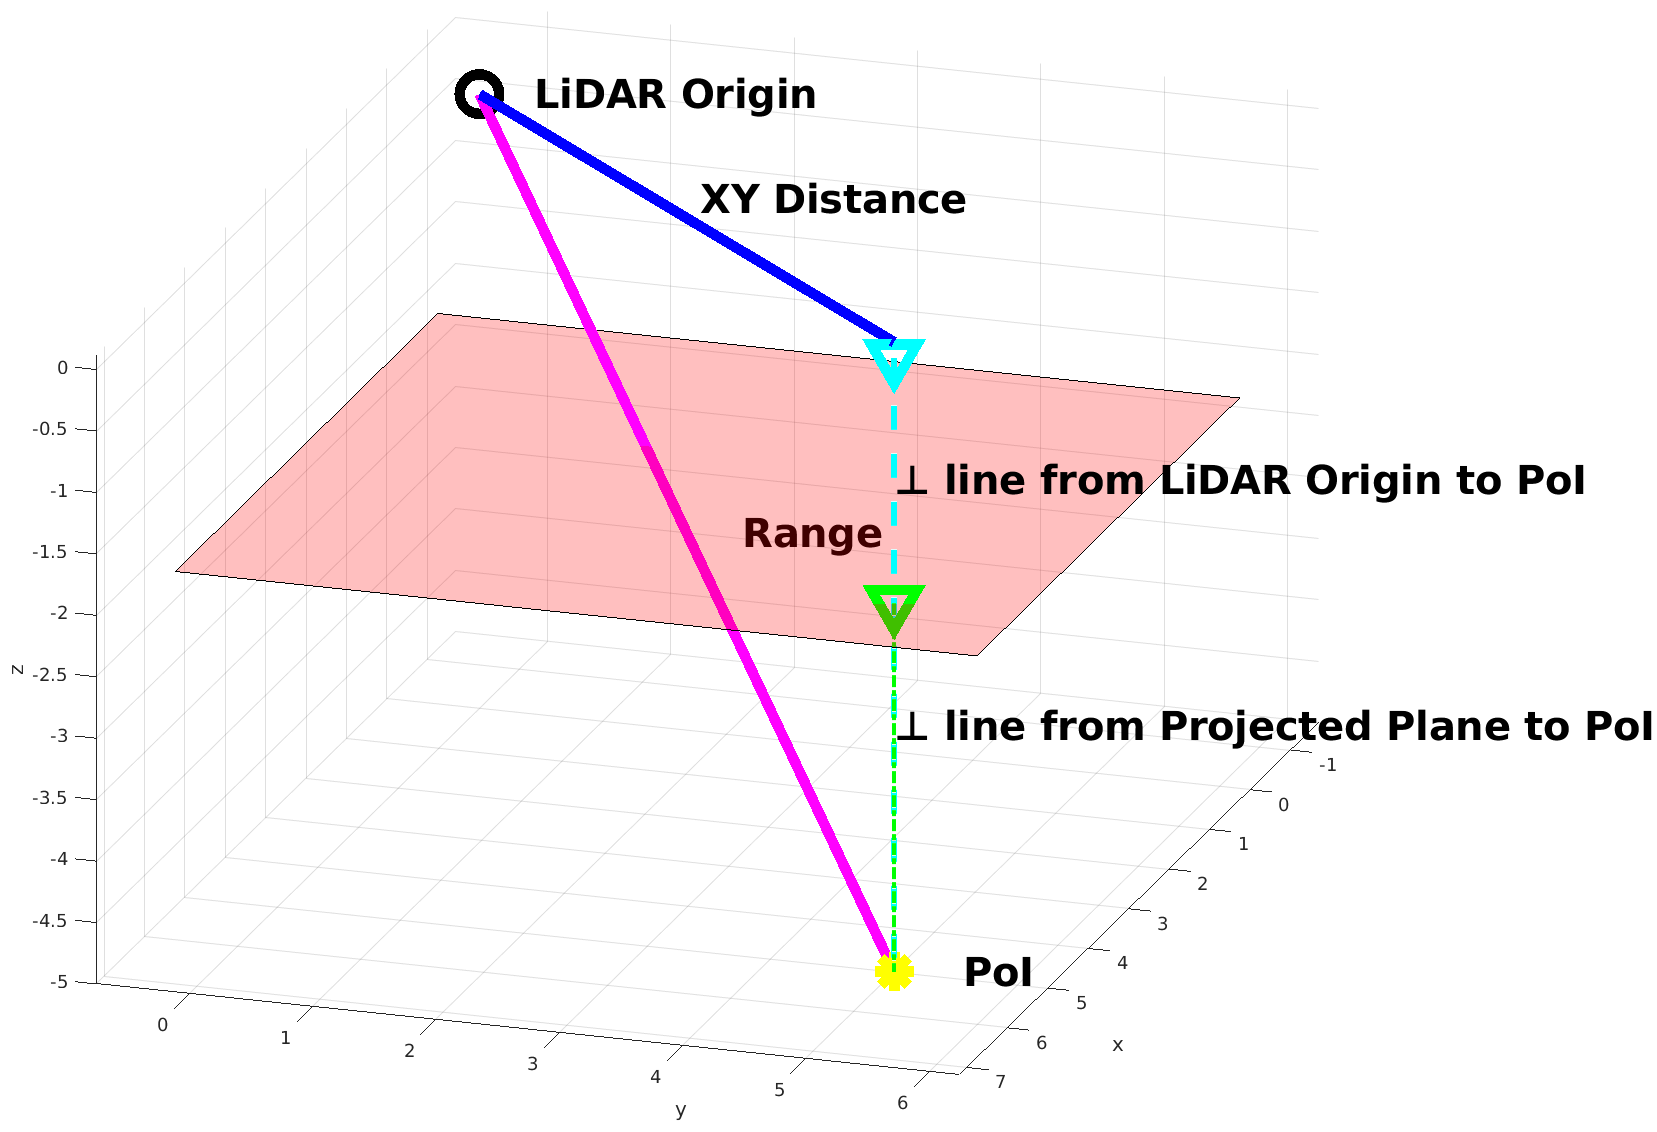
\includegraphics[width=1\linewidth]{Defense_Images/xy_vs_range}
			\caption[XY vs Range vs Z Height]{Two references for feature extraction may be seen in this simplified graph. First is the Range shown by the magenta line from the LiDAR origin to the Point of Interest (PoI). Second is distance from the projected plane (red) to the PoI (green). Mean XY Distance (blue) or Range (magenta) from the sensor was used non-dimensionalize extracted features as needed.}
			\label{fig:xy_vs_range}
		\end{figure}
	
		{Thirty percent of the training data base was randomly selected and set aside as a validation data base. Training data was visually examined for clustering to verify that a Random Decision Forest would be able to be trained (Fig. \ref{fig:range_training_data_cluster_3}). It was found that each class generally clustered to a certain range with some overlap, which indicates that a Random Decision Forest may be trained.}
		
		\begin{figure}[H]
			\centering
			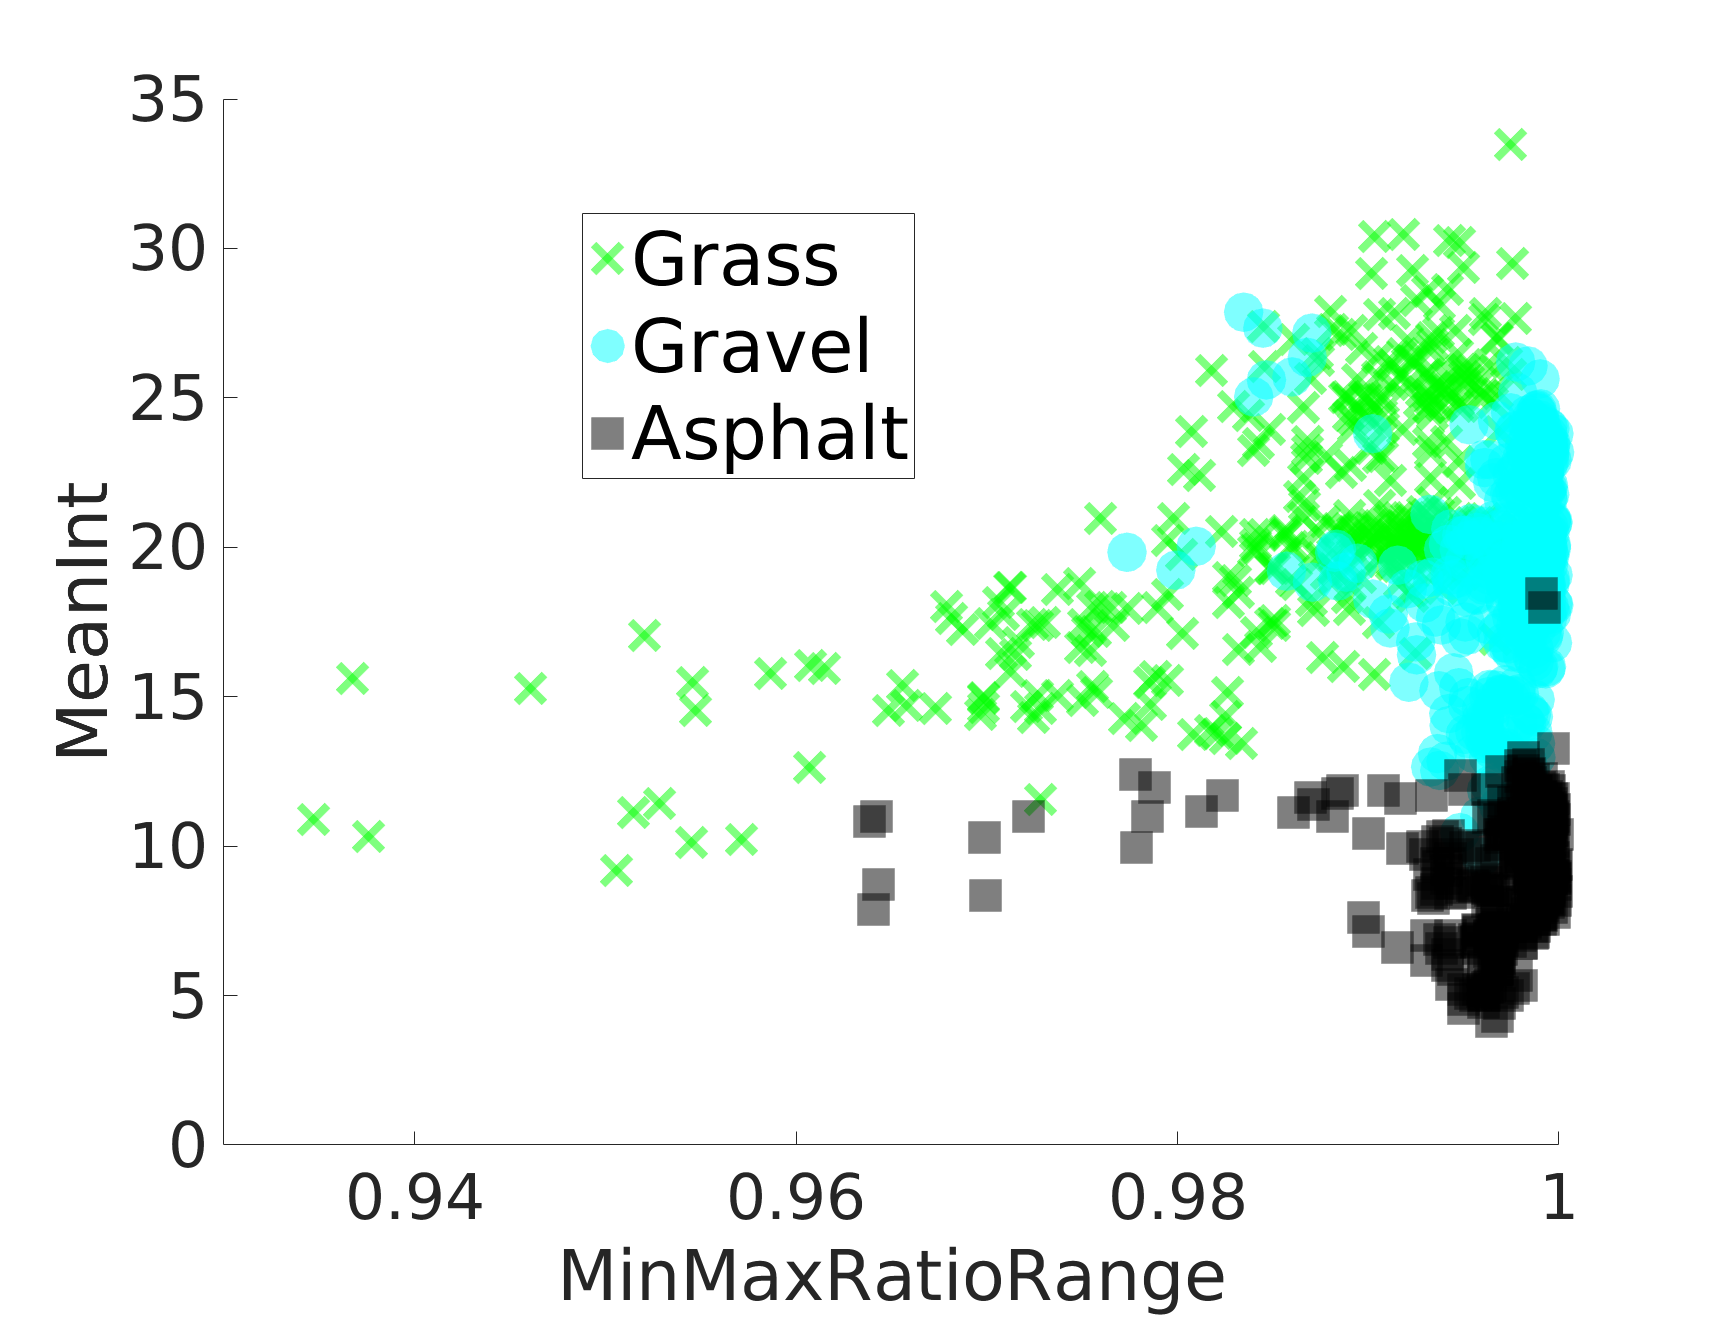
\includegraphics[width=0.75\linewidth]{Defense_Images/training_data_cluster_3}
			\caption[Example Clustering]{Example of training data comparison between two features.}
			\label{fig:range_training_data_cluster_3}
		\end{figure}
		
	} % End Feature Extration
	
	\section{Random Decision Forest Creation}\label{sec:random-decision-forest-creation}{
		
		{MATLAB's Classification Learner Application was used to generate a Random Decision Forests for each considered scanning LiDAR channel. Validation methods for the trained model include Hold-out Validation, Cross Validation, and Resubstitution Validation. Hold-out Validation randomly selects a portion of the training data to train and uses the remainder to validate. Cross Validation divides the training data into partitions or folds. A validation partition is selected, and a model is trained using the remaining folds. Validation error is retained and a new validation partition is selected. The process is repeated until each partition was used for validation. The model with highest accuracy is chosen as the resulting model. Resubstitution Validation, the chosen option, uses all the training data for training and initial validation and does not protect against over-fitting, as well as Cross Validation and Hold-out Validation. This may result in an over-estimation of training accuracy, however as a validation data set was previously made and set aside, further tests will determine if the model is over-fit. Resubstitution Validation was chosen to exactly define the testing and validation data sets, as MATLAB randomly determines the training and validation data sets if other options are chosen, thus reducing reproducibility of results.}
		
		{Random Decision Forest hyper-parameters were tuned to increase terrain classification accuracy. Decision tree depth, number of learners, and number of features to consider for each binary split are hyper-parameters that were optimized using MATLAB's Bayesian Optimization. Bayesian Optimization automates the manual hyper-parameter tuning process by creating a surrogate model representing the objective function, in this case out-of-bag error (Fig. \ref{fig:c2_min_class_error}). Initialization of the objective function is completed by training a number of RDFs using randomly selected hyper-parameters. Out-of-bag error is then found and used to create a series of Gaussian curves. Additional hyper-parameters are chosen by an acquisition function to determine their utility in minimizing out-of-bag error. After a set number of iterations, best hyper-parameters are chosen based minimum upper confidence interval of the classification error objective model. Confusion matrices provide classification accuracy information on training and validation data sets by comparing actual and predicted classes (Fig. \ref{fig:out_of_bag_err_conf_mat}). This process was completed for each of the three considered scanning LiDAR channels used for classification.}
			
		\begin{figure}[H]
			\centering
			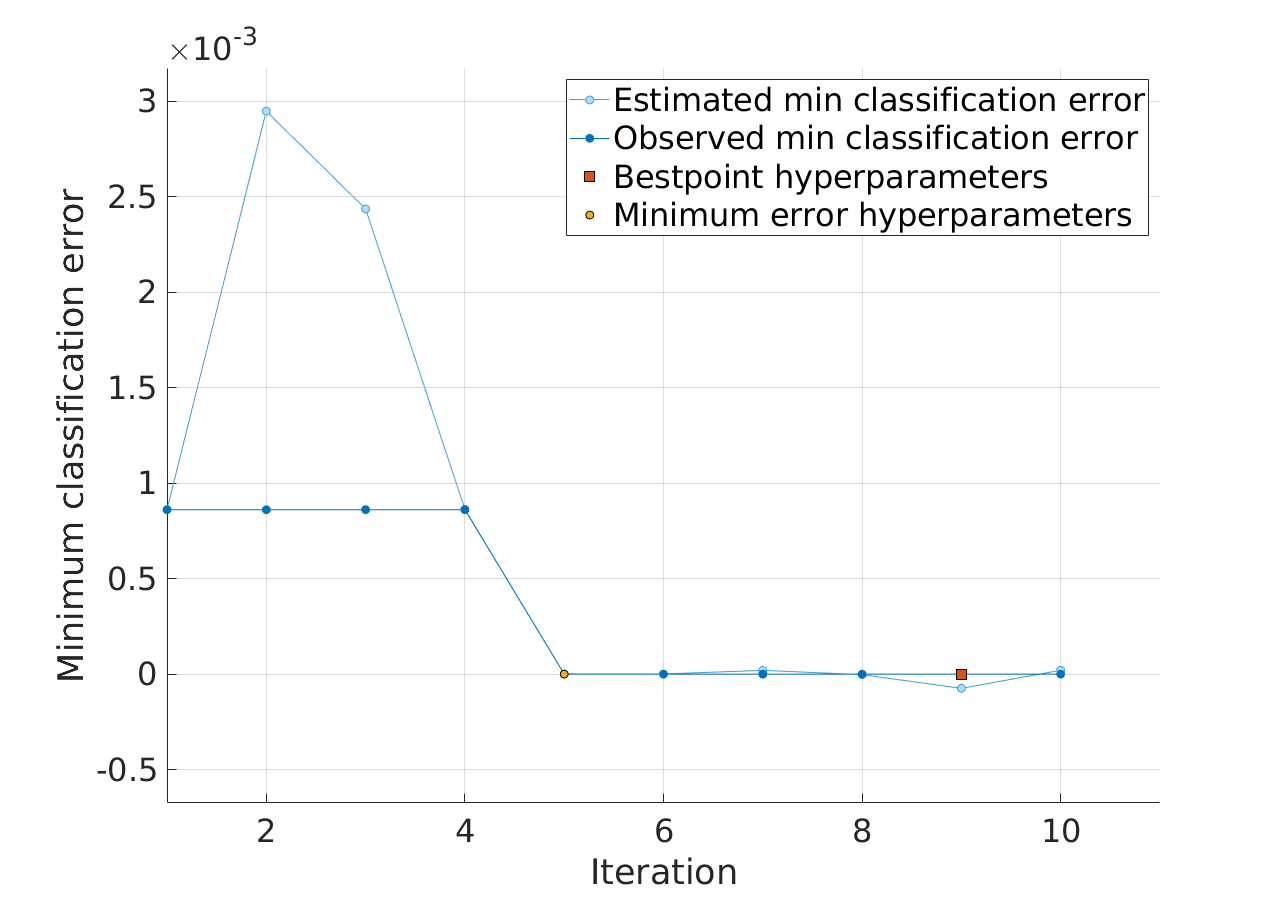
\includegraphics[width=0.5\linewidth]{Defense_Images/c2_bayesian_range}
			\caption[Bayesian Optimization - RANGE]{Classification error during Bayesian Optimization tuning.}
			\label{fig:c2_min_class_error}
		\end{figure}				
		
		\begin{figure}[H]
			\centering
			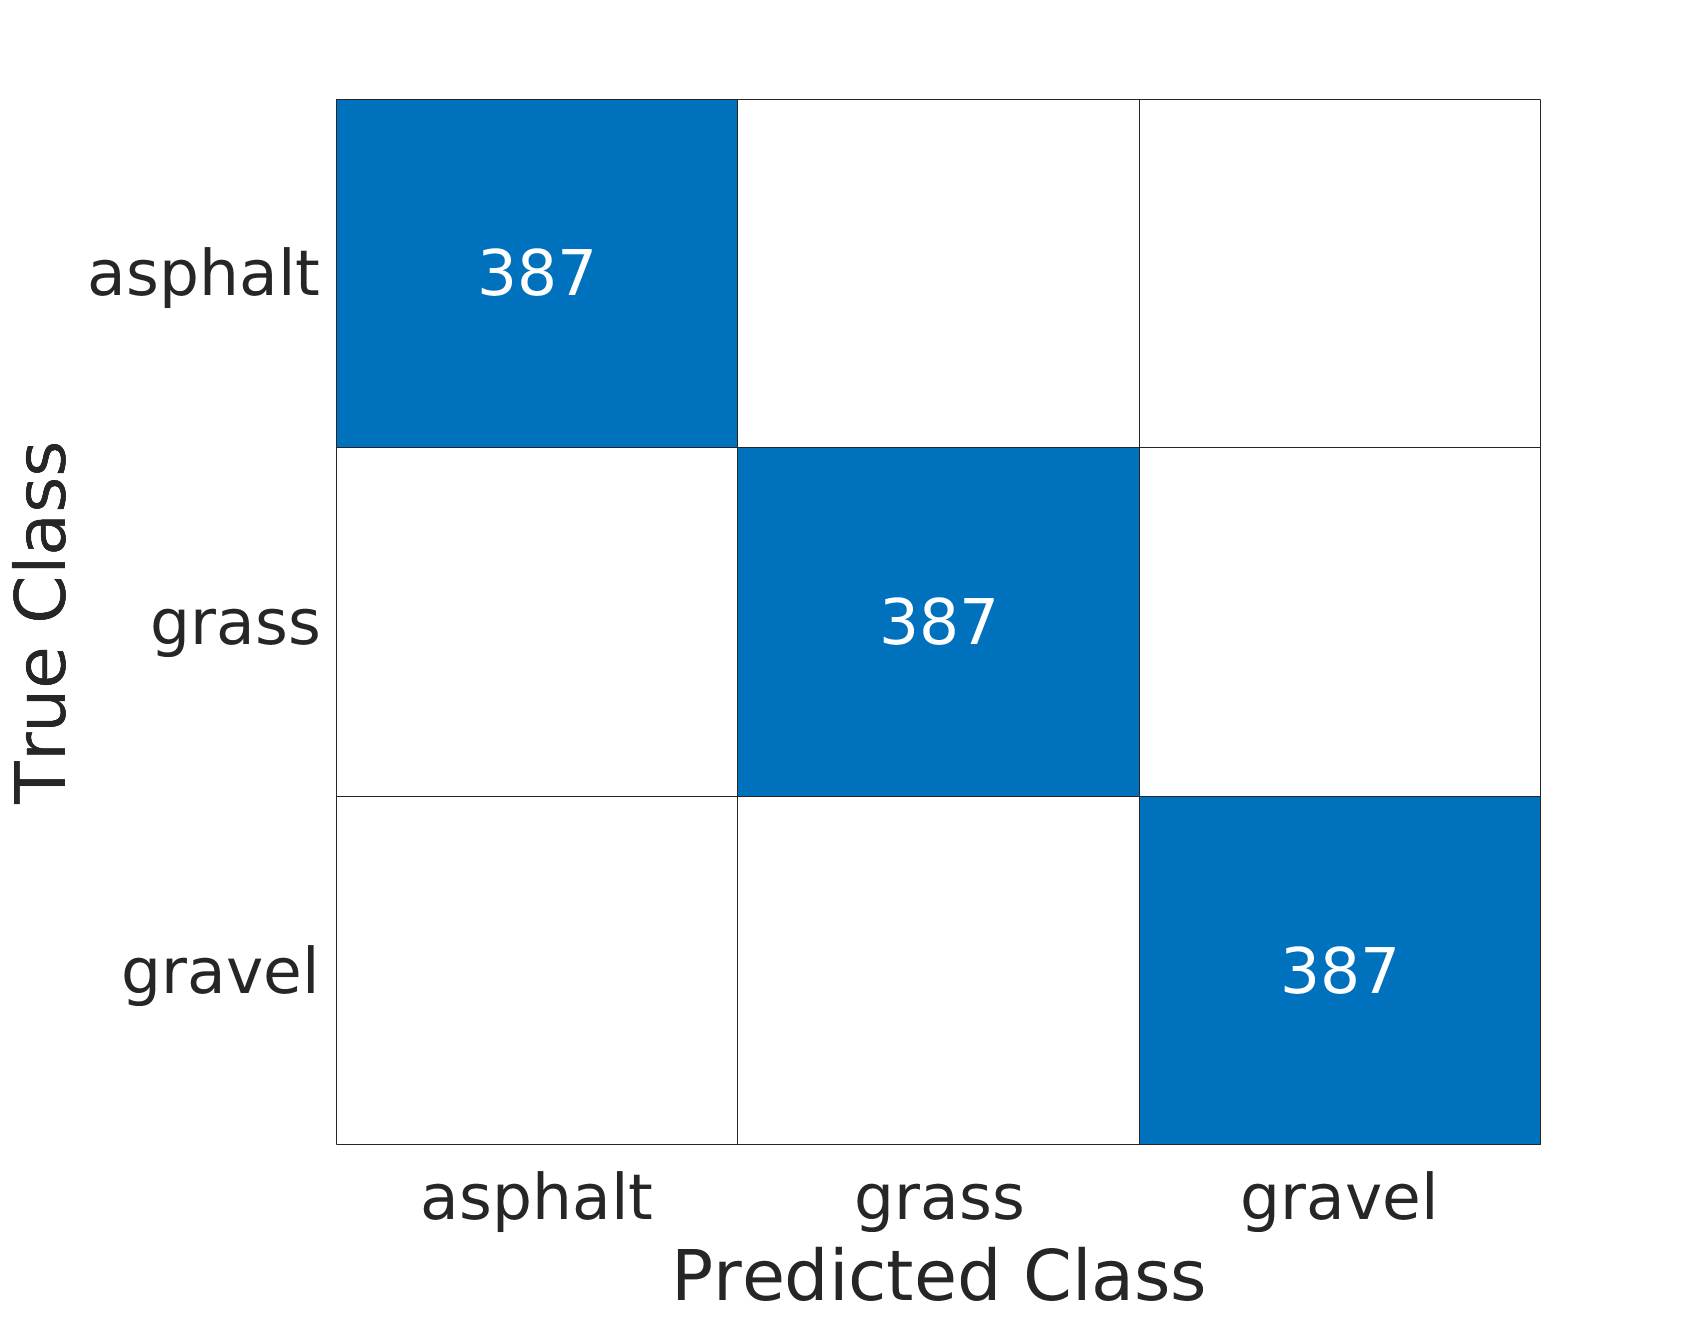
\includegraphics[width=0.65\linewidth]{Defense_Images/chan_2c_conf_OOB_mat222}
			\caption[Out-of-Bag Error]{During training the RDF may be tested using the out-of-bag error. Confusion matrices are used to indicate the final RDF iteration training error. As Resubstitution Validation was used, these results may be too optimistic, therefore further testing was used to ensure that the model did not over-fit.}
			\label{fig:out_of_bag_err_conf_mat}
		\end{figure}
		
		{MATLAB was used to predict the terrain type of arcs of scanning LiDAR data using the $predict$ function, which requires the RDF and the data that is to be tested. Data to be classified was put into table format, as feature column order (Table \ref{tab:Training_Data_Example}) does not matter, and any additional columns that the RDF was not trained on is ignored.}
		
		\begin{table}[H]
			\centering
			\begin{tabular}{ >{\centering}p{3.0cm} >{\centering}p{0.25cm} >{\centering}p{1.5cm} >{\centering}p{1.5cm} >{\centering}p{1.5cm} }
				\textbf{Terrain Types}                       	&                       & \multicolumn{3}{c}{\textbf{Training Data}}                                                                         \tabularnewline \cline{1-1} \cline{3-5} 
				\multicolumn{1}{|c|}{\textit{Classification}} 	& \multicolumn{1}{c|}{} & \multicolumn{1}{c|}{\textit{Feat 1}} & \multicolumn{1}{c|}{\textit{Feat 2}} & \multicolumn{1}{c|}{\textit{Feat 3}} \tabularnewline \cline{1-1} \cline{3-5} 
				\multicolumn{1}{|c|}{gravel}                  	& \multicolumn{1}{c|}{} & \multicolumn{1}{c|}{1}               & \multicolumn{1}{c|}{2}               & \multicolumn{1}{c|}{3}               \tabularnewline \cline{1-1} \cline{3-5} 
				\multicolumn{1}{|c|}{asphalt}                	& \multicolumn{1}{c|}{} & \multicolumn{1}{c|}{4}               & \multicolumn{1}{c|}{5}               & \multicolumn{1}{c|}{6}               \tabularnewline \cline{1-1} \cline{3-5} 
				\multicolumn{1}{|c|}{unknown}                	& \multicolumn{1}{c|}{} & \multicolumn{1}{c|}{7}               & \multicolumn{1}{c|}{8}               & \multicolumn{1}{c|}{9}               \tabularnewline \cline{1-1} \cline{3-5} 
			\end{tabular}
			\caption[Training Data Input Argument Example]{Simple example of class label table and training data table.}
			\label{tab:Training_Data_Example}
		\end{table}
		
		\lstinputlisting[style=Matlab-editor, basicstyle=\mlttfamily\scriptsize, caption={Predict function example with intput and output arguments}]{y_fit_example.m}
		
		{Class prediction is yielded in $Yfit$. Scores for each class type in percent probability is given in $scores$, of which the highest score dictates $Yfit$. Standard deviations of predicted classification is given in $stdevs$. For this work, $Yfit$  and $scores$ were used for testing.}

		
	} % End Random Decision Forest Creation


	\section{Random Decision Forest Testing}\label{sec:random-decision-forest-verification}{
	
		{Random Decision Forest classification accuracy was verified by passing the algorithm a verification data set. Thirty percent of the training data base was randomly selected and set aside to create the verification data base. Confusion matrices provide classification accuracy information on validation database by classifying each data set in the validation database and comparing actual and predicted classes, resulting in a matrix that visualizes the accuracy for each terrain type as well as which terrain types are more likely to be confused for a different class (Fig. \ref{fig:vali_err_conf_mat_range}). Hyperparameter tuning may lead to over-fitting to the training data base. Testing for over-fitting was accomplished by comparing the out-of-bag training error to the validation error (Fig. \ref{fig:train_vs_valid_overfit_test2}). This process was completed for each of the three considered scanning LiDAR channels used for classification. }
						
		\begin{figure}[H]
			\centering
			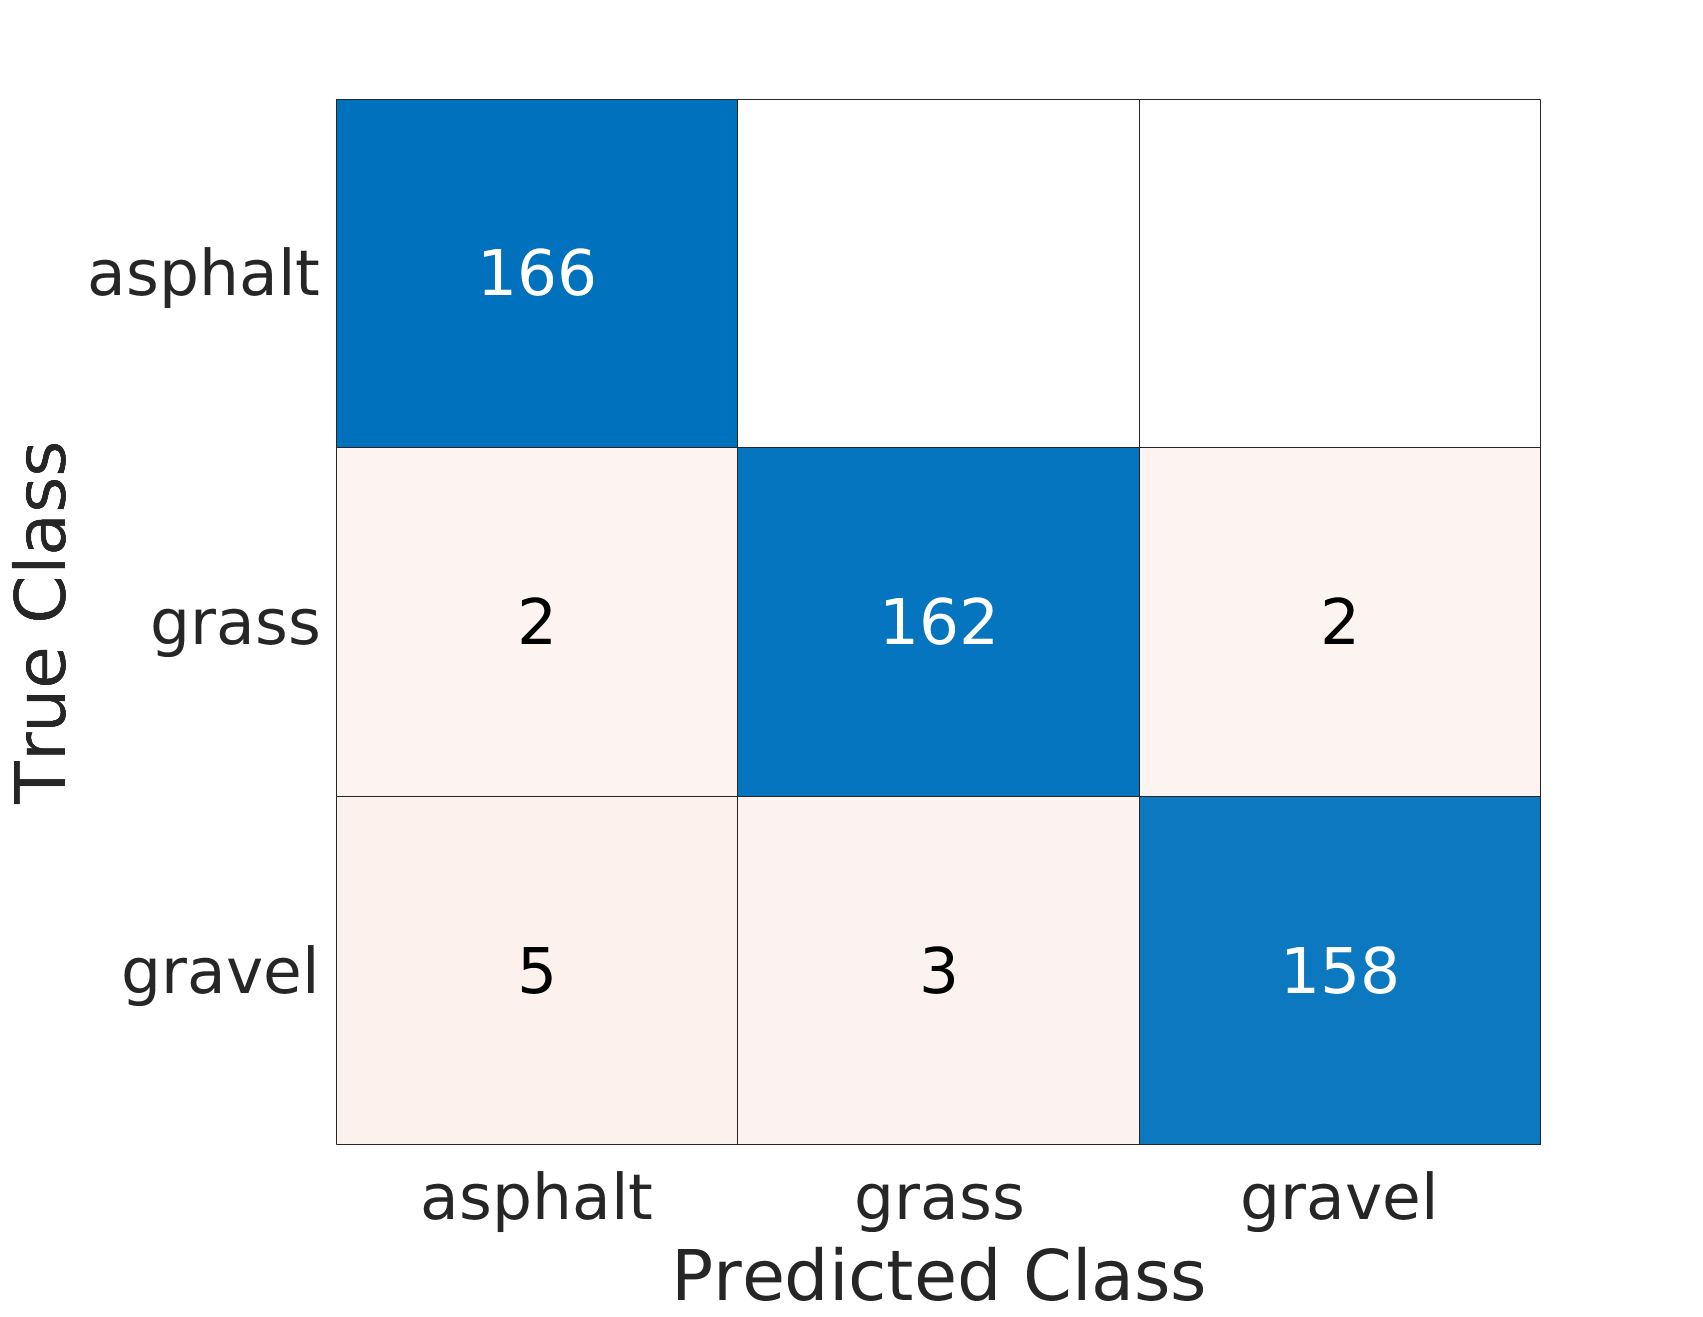
\includegraphics[width=0.65\linewidth]{Defense_Images/chan_2c_conf_VALIDATION_mat222}
			\caption[Validation Error]{Confusion matrix with the validation training data set.}
			\label{fig:vali_err_conf_mat_range}
		\end{figure}
	
		\begin{figure}[H]
			\centering
			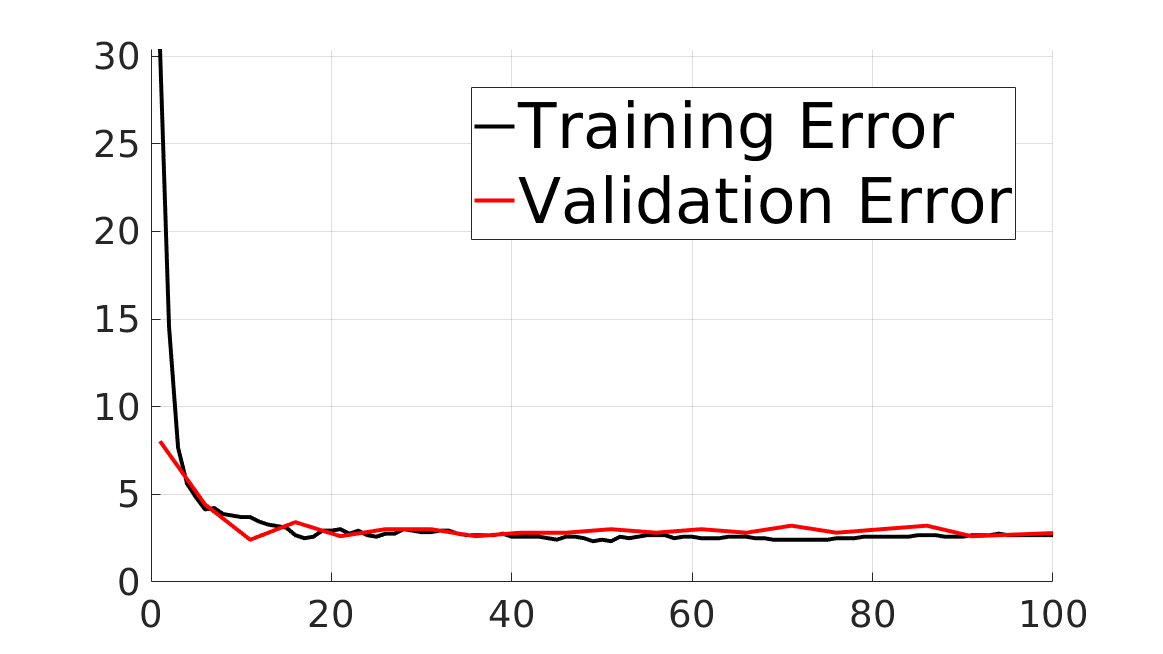
\includegraphics[width=0.75\linewidth]{Defense_Images/train_vs_valid_overfit_test2}
			\caption[Training vs Validation Error]{Out-of-bag training- versus validation-error for the range-based channel 2 RDF. Hyperparameter tuning may lead to over-fitting. Testing out-of-bag versus validation error demonstrates that the model is not over-fitting to the training data base the validation error does not diverge from the out-of-bag error.}
			\label{fig:train_vs_valid_overfit_test2}
		\end{figure}
			


	} % End Random Decision Forest Verification
	


	\section{Consecutive Point Cloud Classification}\label{sec:consecutive_point_cloud_classification}{
	
		{Classifying consecutive LiDAR scans was accomplished by examination of the nine arcs of interest in front and forty-five degree angles left and right from the front of the experimental apparatus (Figure \ref{fig:area_example}). Features from each arc were extracted and the arcs were classified using the derived Random Decision Forest algorithms in Objective 1. Point coordinates in each arc were averaged to represent each arc as a single point. GPS and IMU data with closest matching timestamps to consecutive LiDAR scans were used to create the transformation matrix derivation in the process described in \ref{sec:aggregating_point_cloud_data} and applied to the classified points. LiDAR scans were then compiled into a single classified point cloud (Figure \ref{fig:db_1_all_points_example_withvan}). To simplify classification accuracy scoring, average coordinates of each classified arc were calculated (Figure \ref{fig:all_to_avg}), allowing for the determination of scores based off averaged location of each arc (Section \ref{sec:consecutive_point_cloud_classification_scoring}).}
		
		\begin{figure}[H]
			\centering
			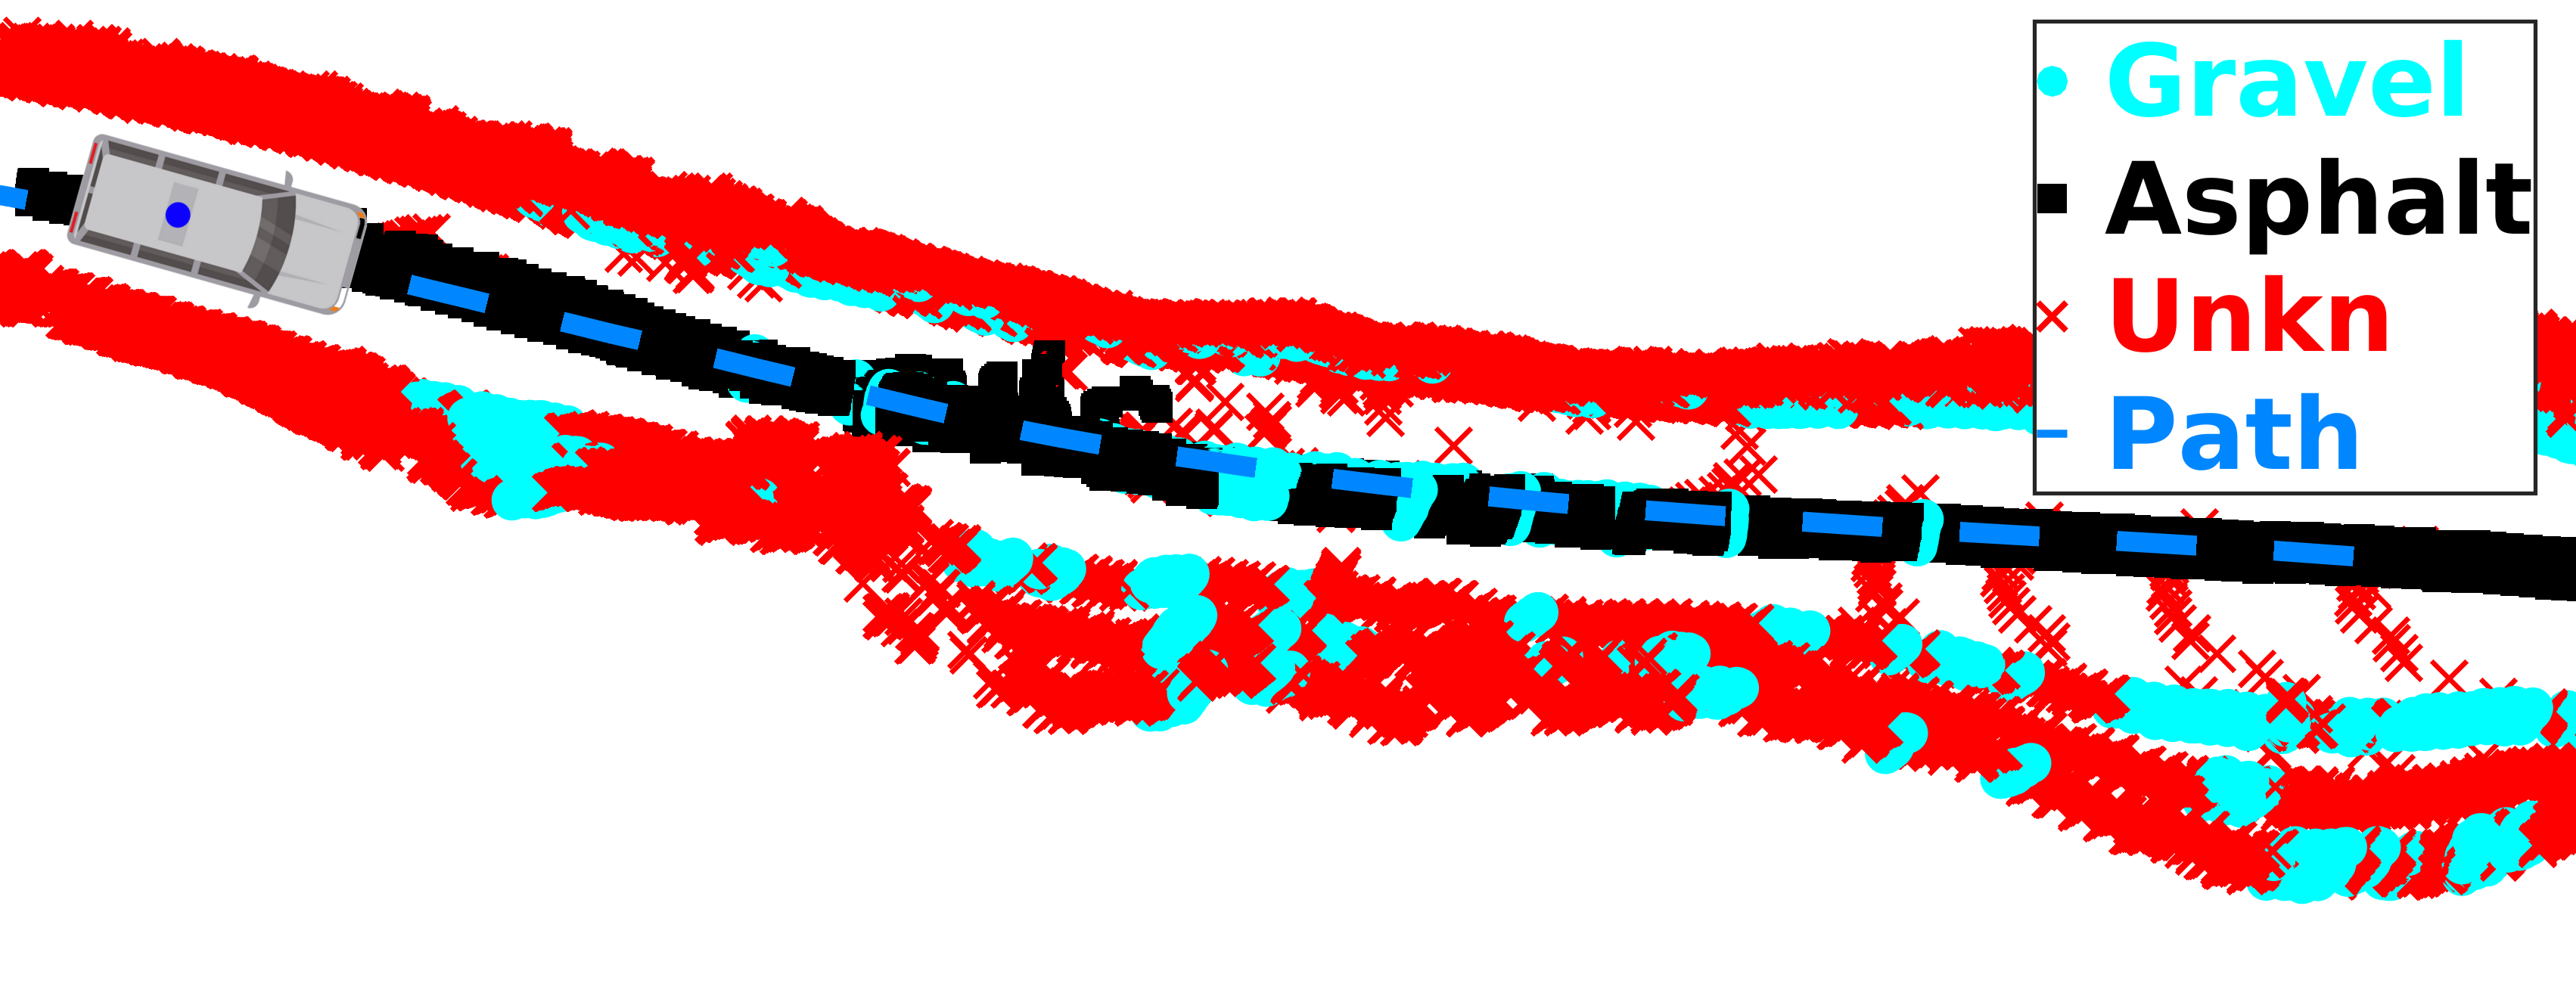
\includegraphics[width=0.9\linewidth]{Defense_Images/db_1_all_points_example_withvan}
			\caption[Classified Point Cloud]{Typical example of a classified point cloud. Vehicle path is highlighted as a dashed line.}
			\label{fig:db_1_all_points_example_withvan}
		\end{figure}
		
		\begin{figure}[H]
			\centering
			\begin{subfigure}{0.45\textwidth}
				\centering
				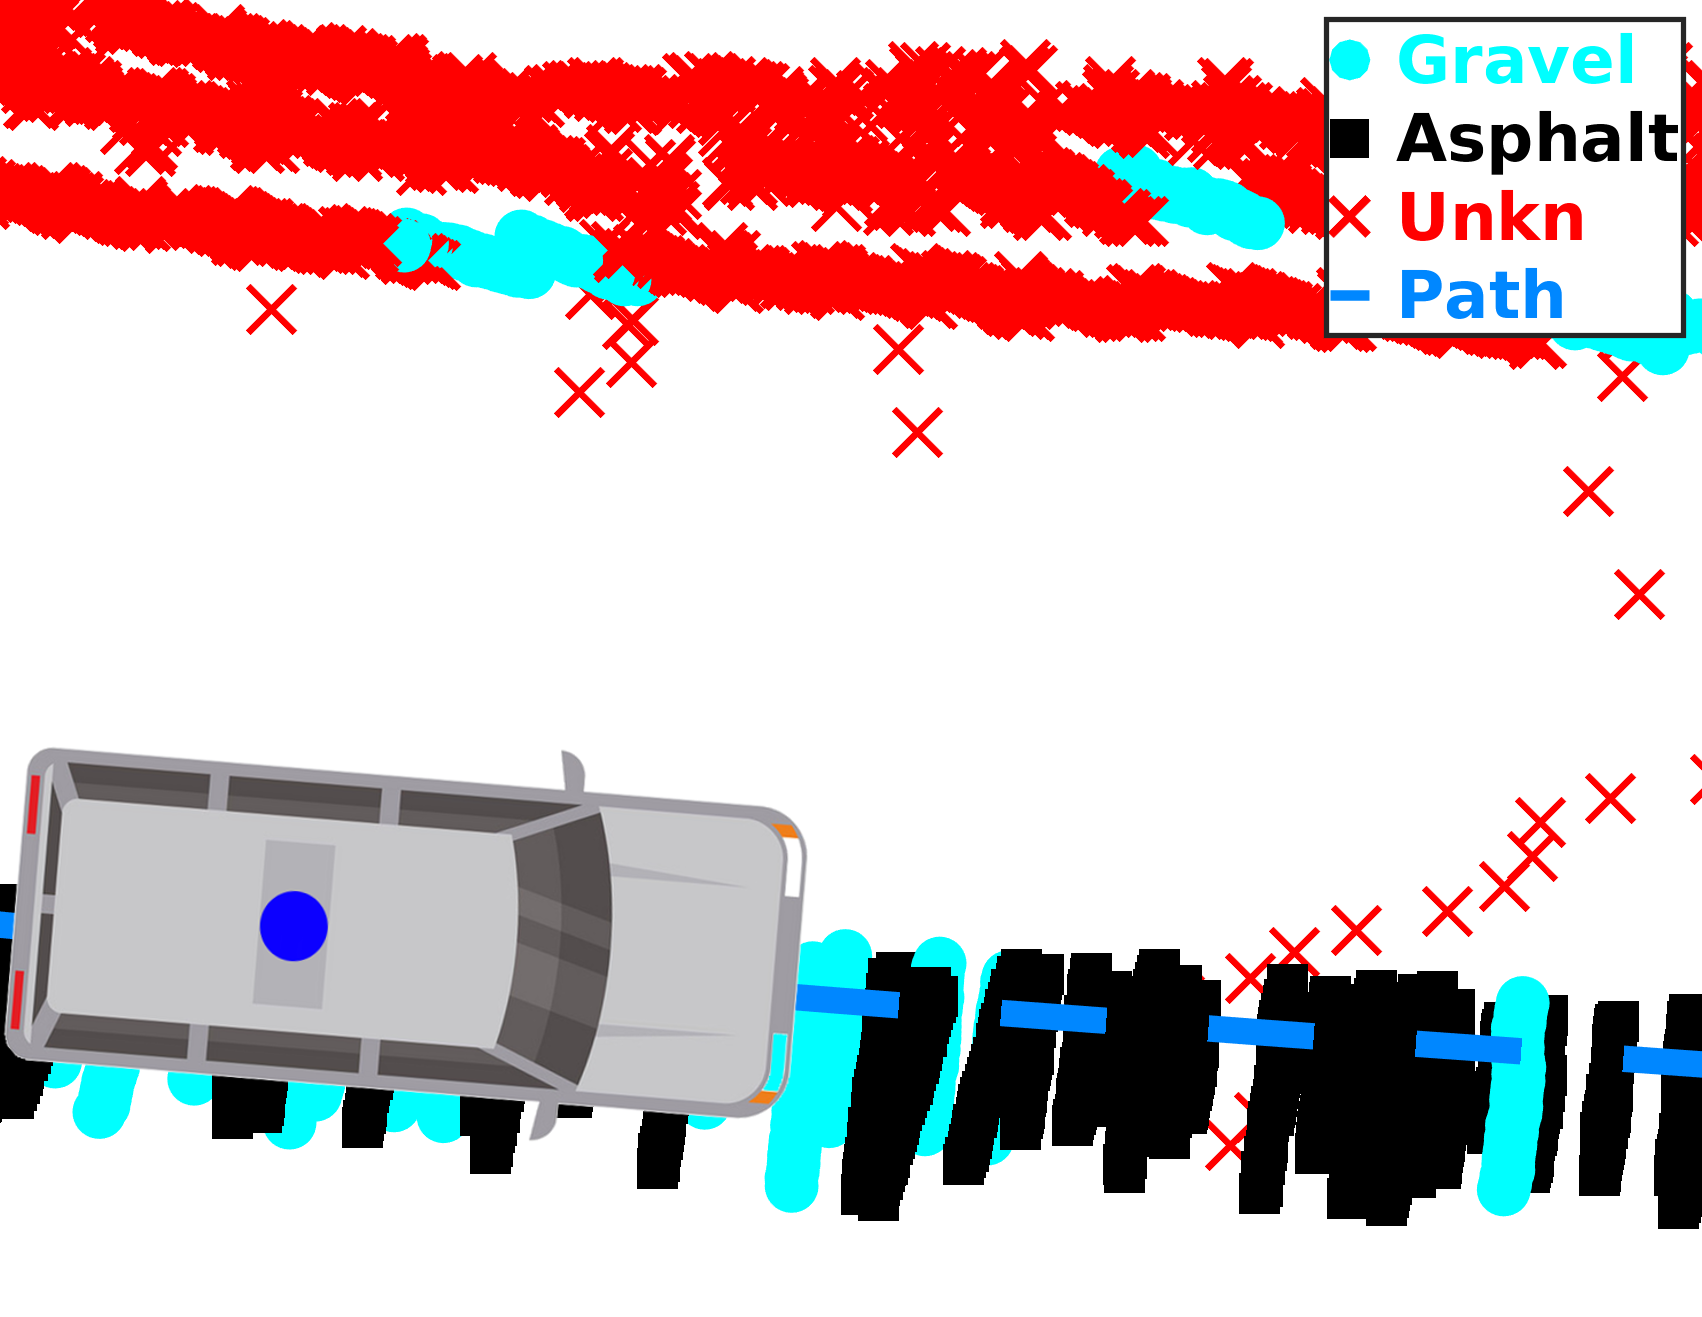
\includegraphics[width=1.0\linewidth]{Defense_Images/all_points_example_withvan}
				\caption[]{}
				\label{fig:all_points_example_withvan}
			\end{subfigure}
			\begin{subfigure}{0.45\textwidth}
				\centering
				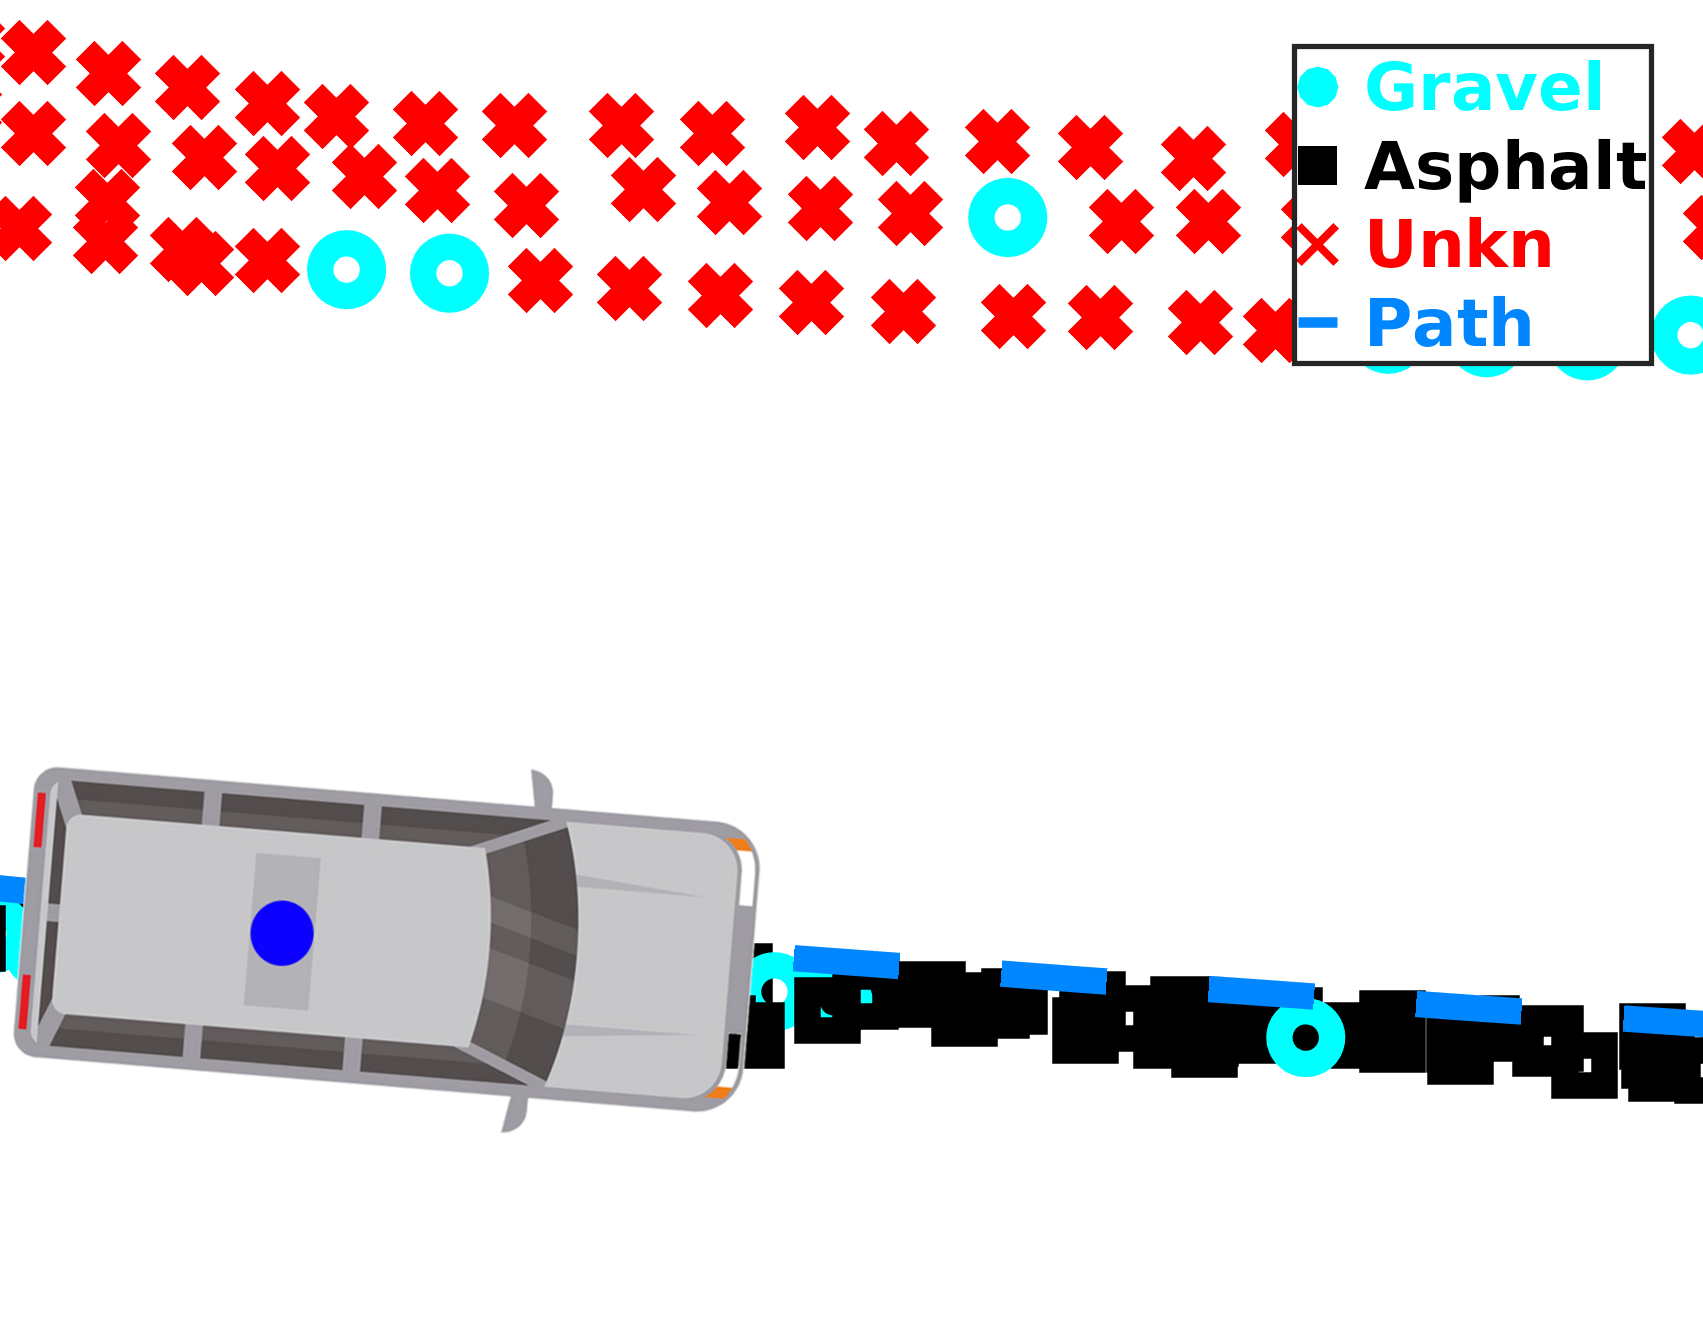
\includegraphics[width=1.0\linewidth]{Defense_Images/avg_points_example_withvan}
				\caption[]{}
				\label{fig:avg_points_example_withvan}
			\end{subfigure}
			\caption[Average Arc Coordinate Cloud Creation]{Entire arcs of classified points (a) may be simplified to a single point (b), allowing for simpler scoring processes and easier visual interpretation of results. }
			\label{fig:all_to_avg}
		\end{figure}
		
		\begin{figure}[H]
			\centering
			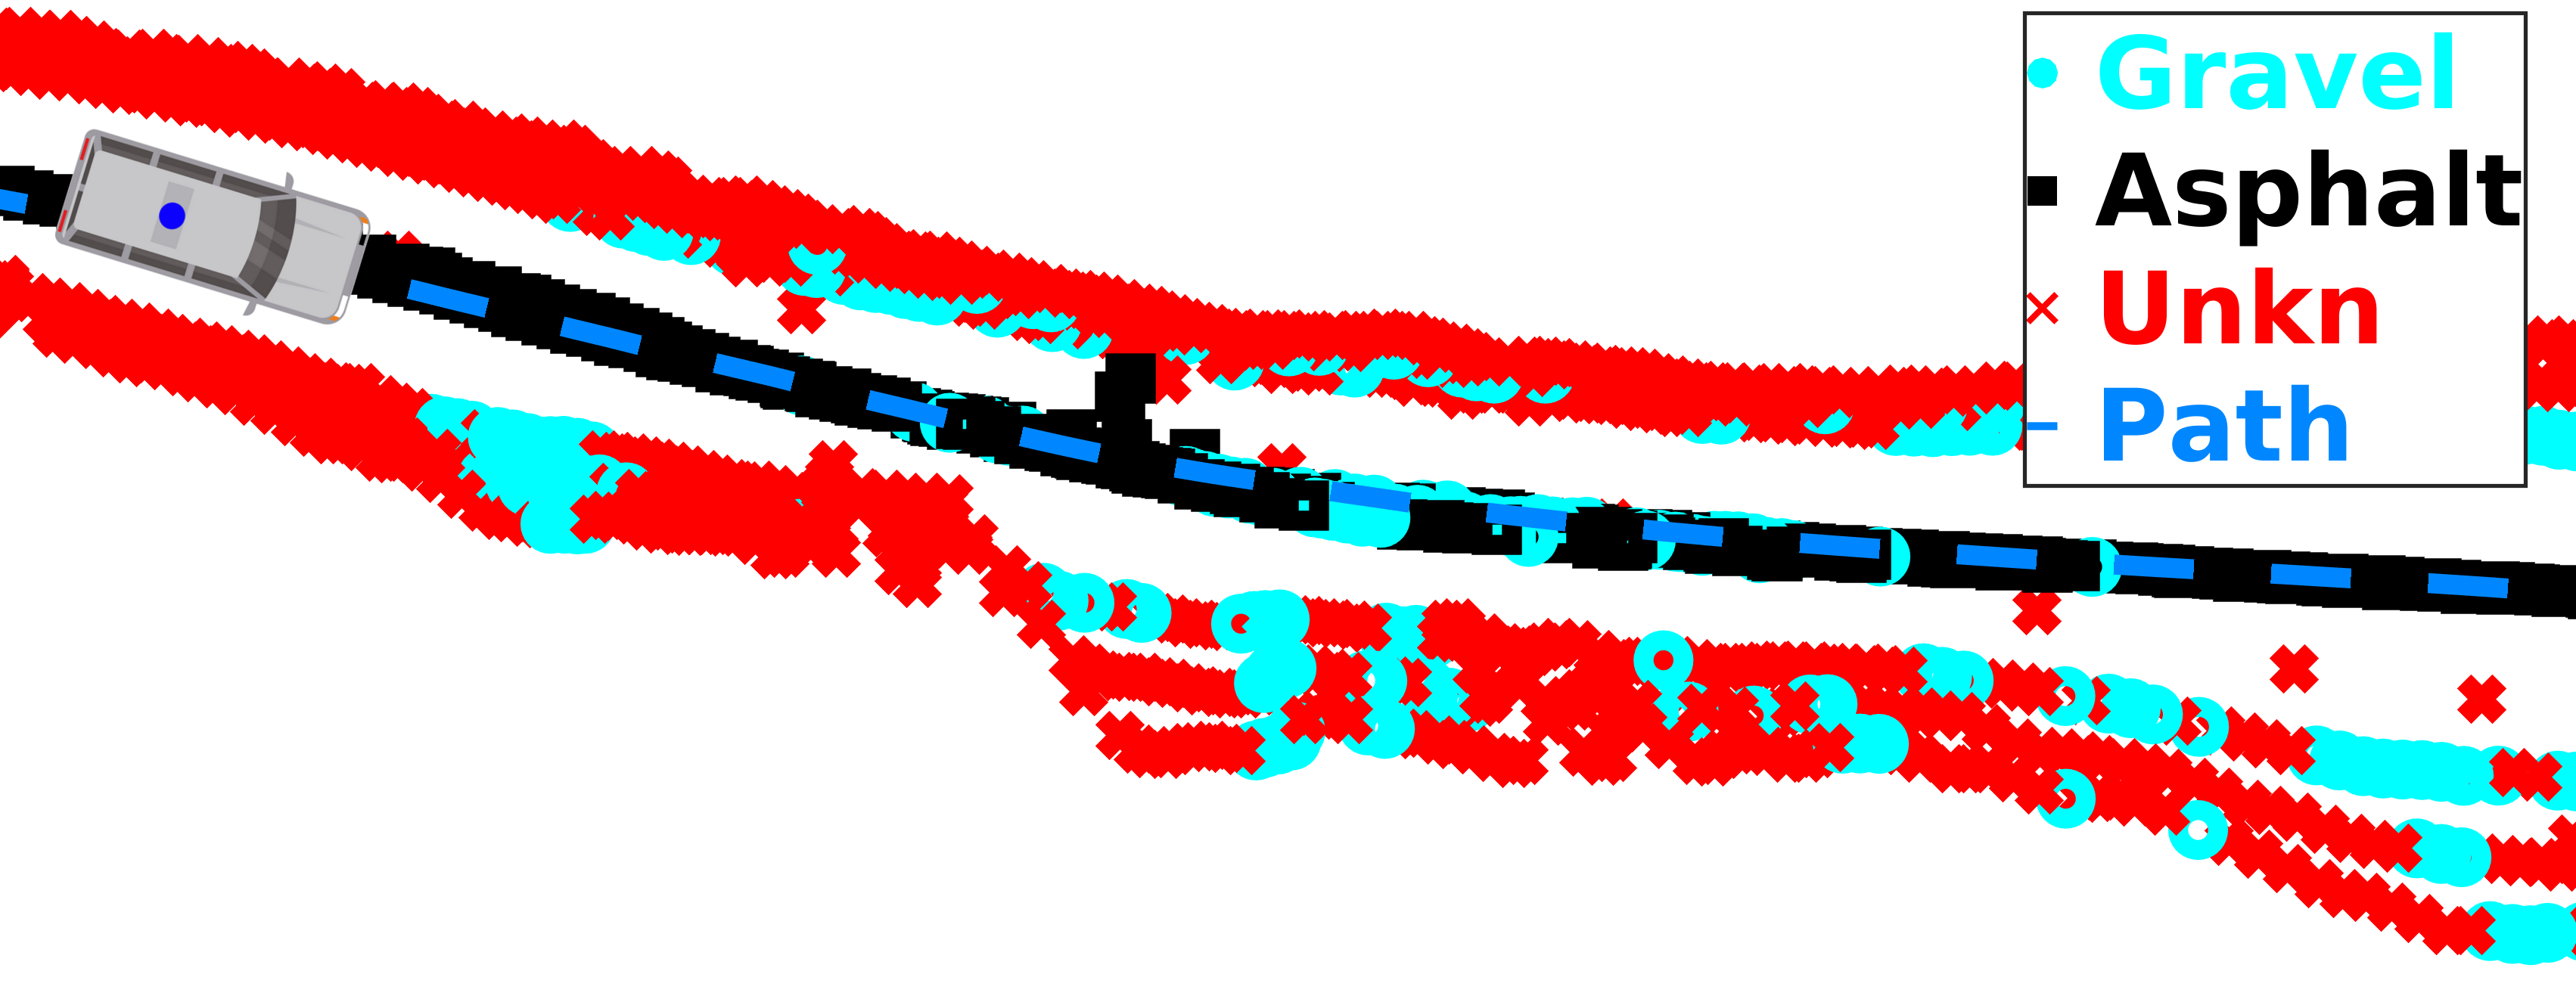
\includegraphics[width=0.9\linewidth]{Defense_Images/db_1_avg_points_example_withvan}
			\caption[Classified Point Cloud]{Typical example of a classified point cloud using averaged coordinates of each classified arc. Vehicle path is highlighted as a dashed line.}
			\label{fig:raw_classification_results}
		\end{figure}
		
	}
	
	\section{Consecutive Point Cloud Classification Scoring}\label{sec:consecutive_point_cloud_classification_scoring}{
		
		{Scoring results was accomplished by comparing the aggregated classified point cloud to manually defined areas. Manually defined areas were derived using the process described in \ref{sec:training_and_verification_data_selection_process}. Gravel, asphalt, and side-of-road truth areas were projected onto a point cloud comprised of the averaged x, y, and z coordinates of each arc for the determination of classification accuracy (Fig. \ref{fig:rm_db_1_area_score}). Classification results that were sympatric to manually defined areas were extracted and examined for accuracy. Accuracy scores was calculated based on the distribution of classified points with each area, allowing evaluation of unmarked road detection performance. Road detection accuracy was determined by scoring the exact terrain classification, true positive road surface detection, and false negative road surface detection. Side-of-road areas were considered for road edge detection. Drop off in positive road surface classification rates in side-of-road areas would be indicative that the random decision forest classification algorithm was adequate at detecting the road edge.}
		
		% IMAGE FOR CLASSIFIED PIONTS VS AREAS

		\begin{figure}[H]
			\centering
			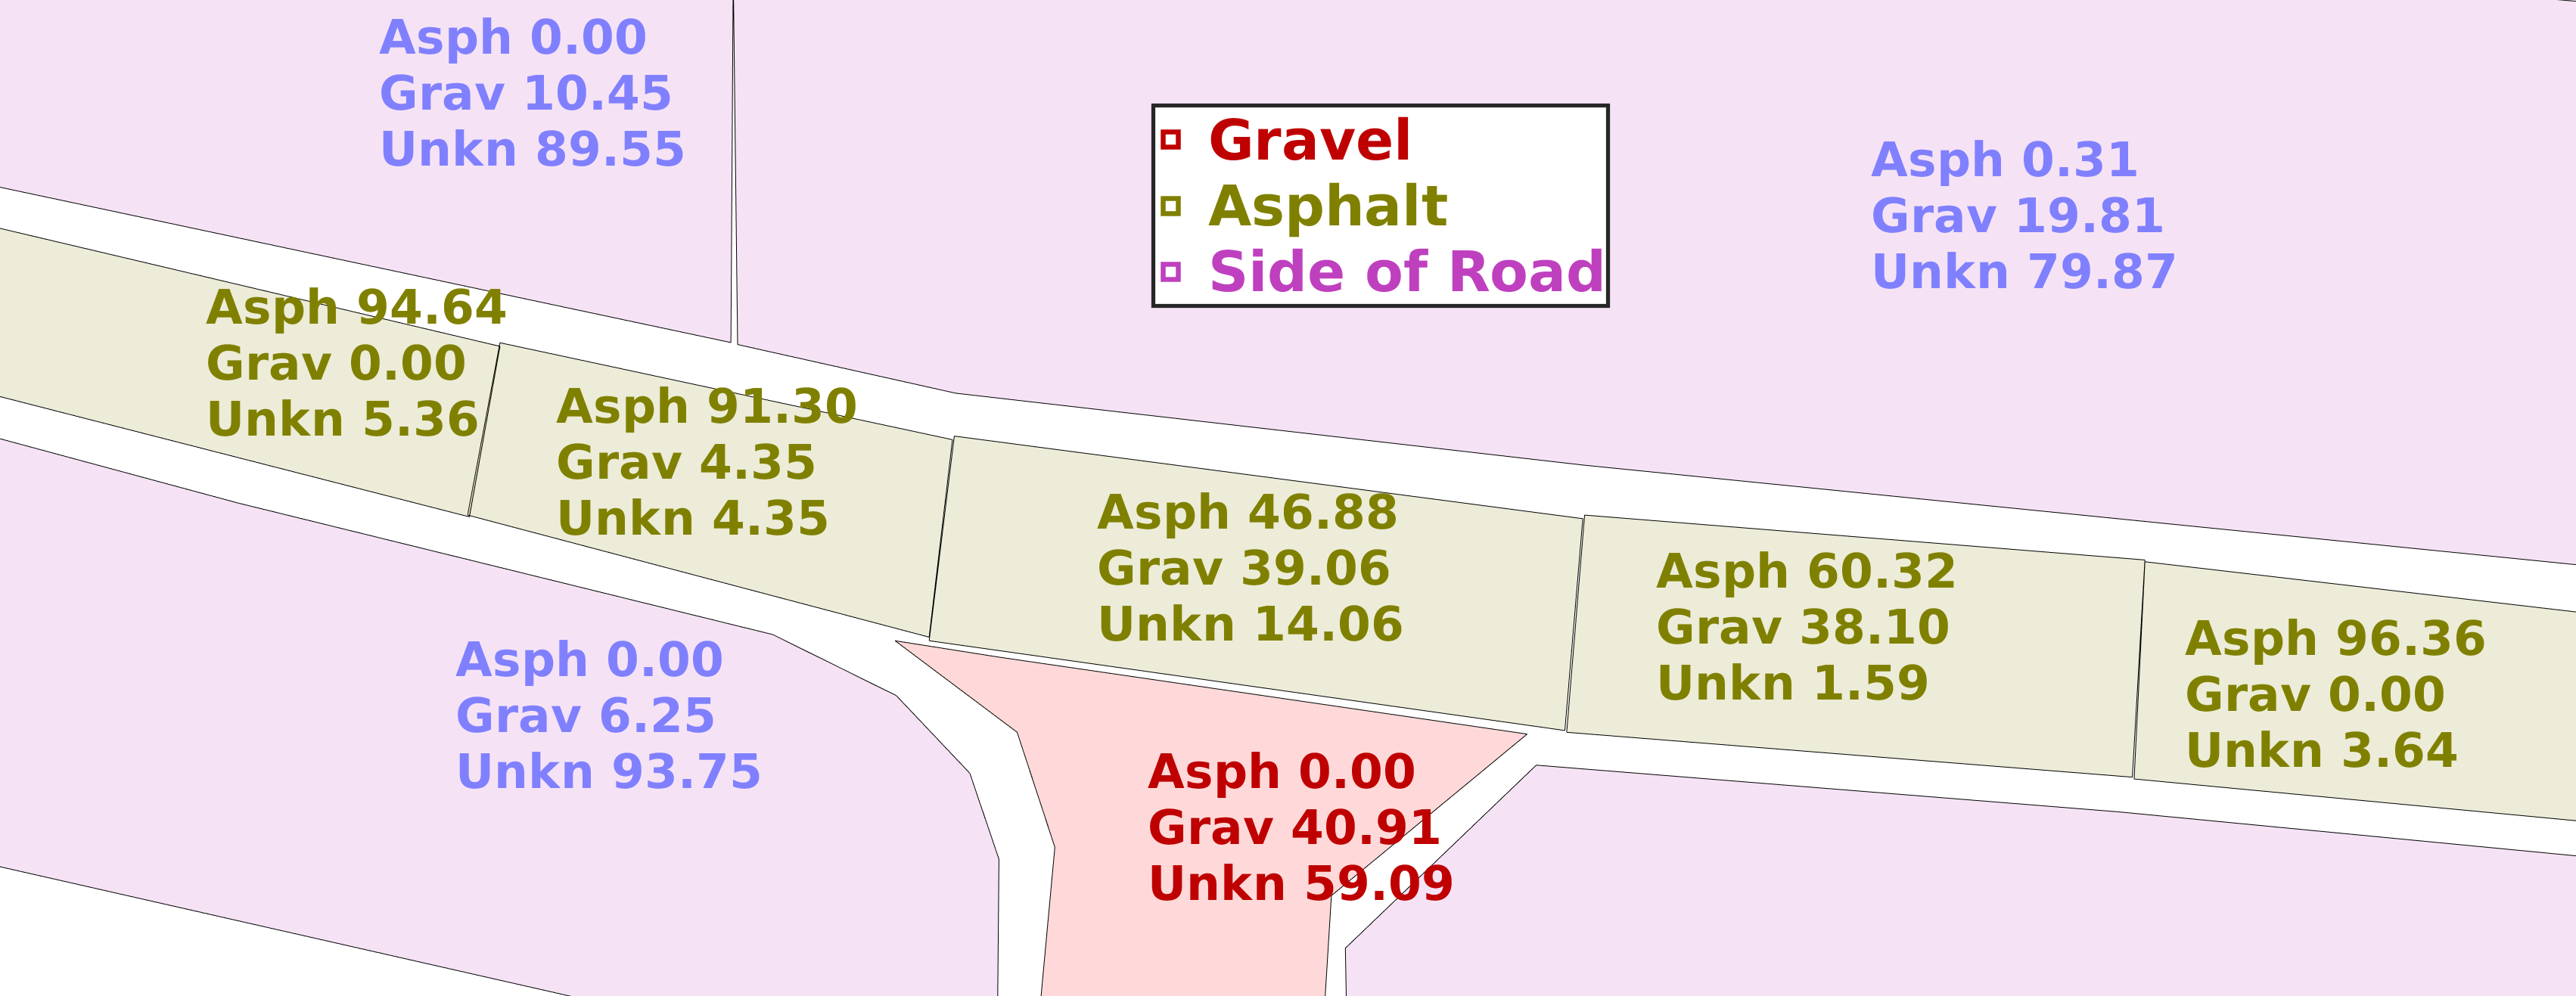
\includegraphics[width=0.90\linewidth]{Defense_Images/rm_db_1_area_score}
			\caption[Area Scores]{Per-area scores were calculated, indicating algorithm unmarked road detection accuracy. }
			\label{fig:rm_db_1_area_score}
		\end{figure}

		
	}

	\section{Visual Road Detection}\label{sec:manual_road_detection}{
	
		{Classified point clouds were visually inspected to determine if the manual detection of a road surface may be accomplished. If consecutive points from each channel in any direction had two or more matching gravel or asphalt classification and was evenly spaced, a gravel or asphalt road surface area was projected. Guessed road surface areas were then compared to actual areas to determine the method's ability at unmarked gravel road discovery, indicating the method's efficiency at detecting intercepting gravel roads (Figure \ref{fig:rm_db_6_overlap_2}). Individual drive ways were scored individually, while non-overlapping areas were compiled to determine the average rate of false-positive identifications for road surfaces.}	
		
		\begin{figure}[H]
			\centering
			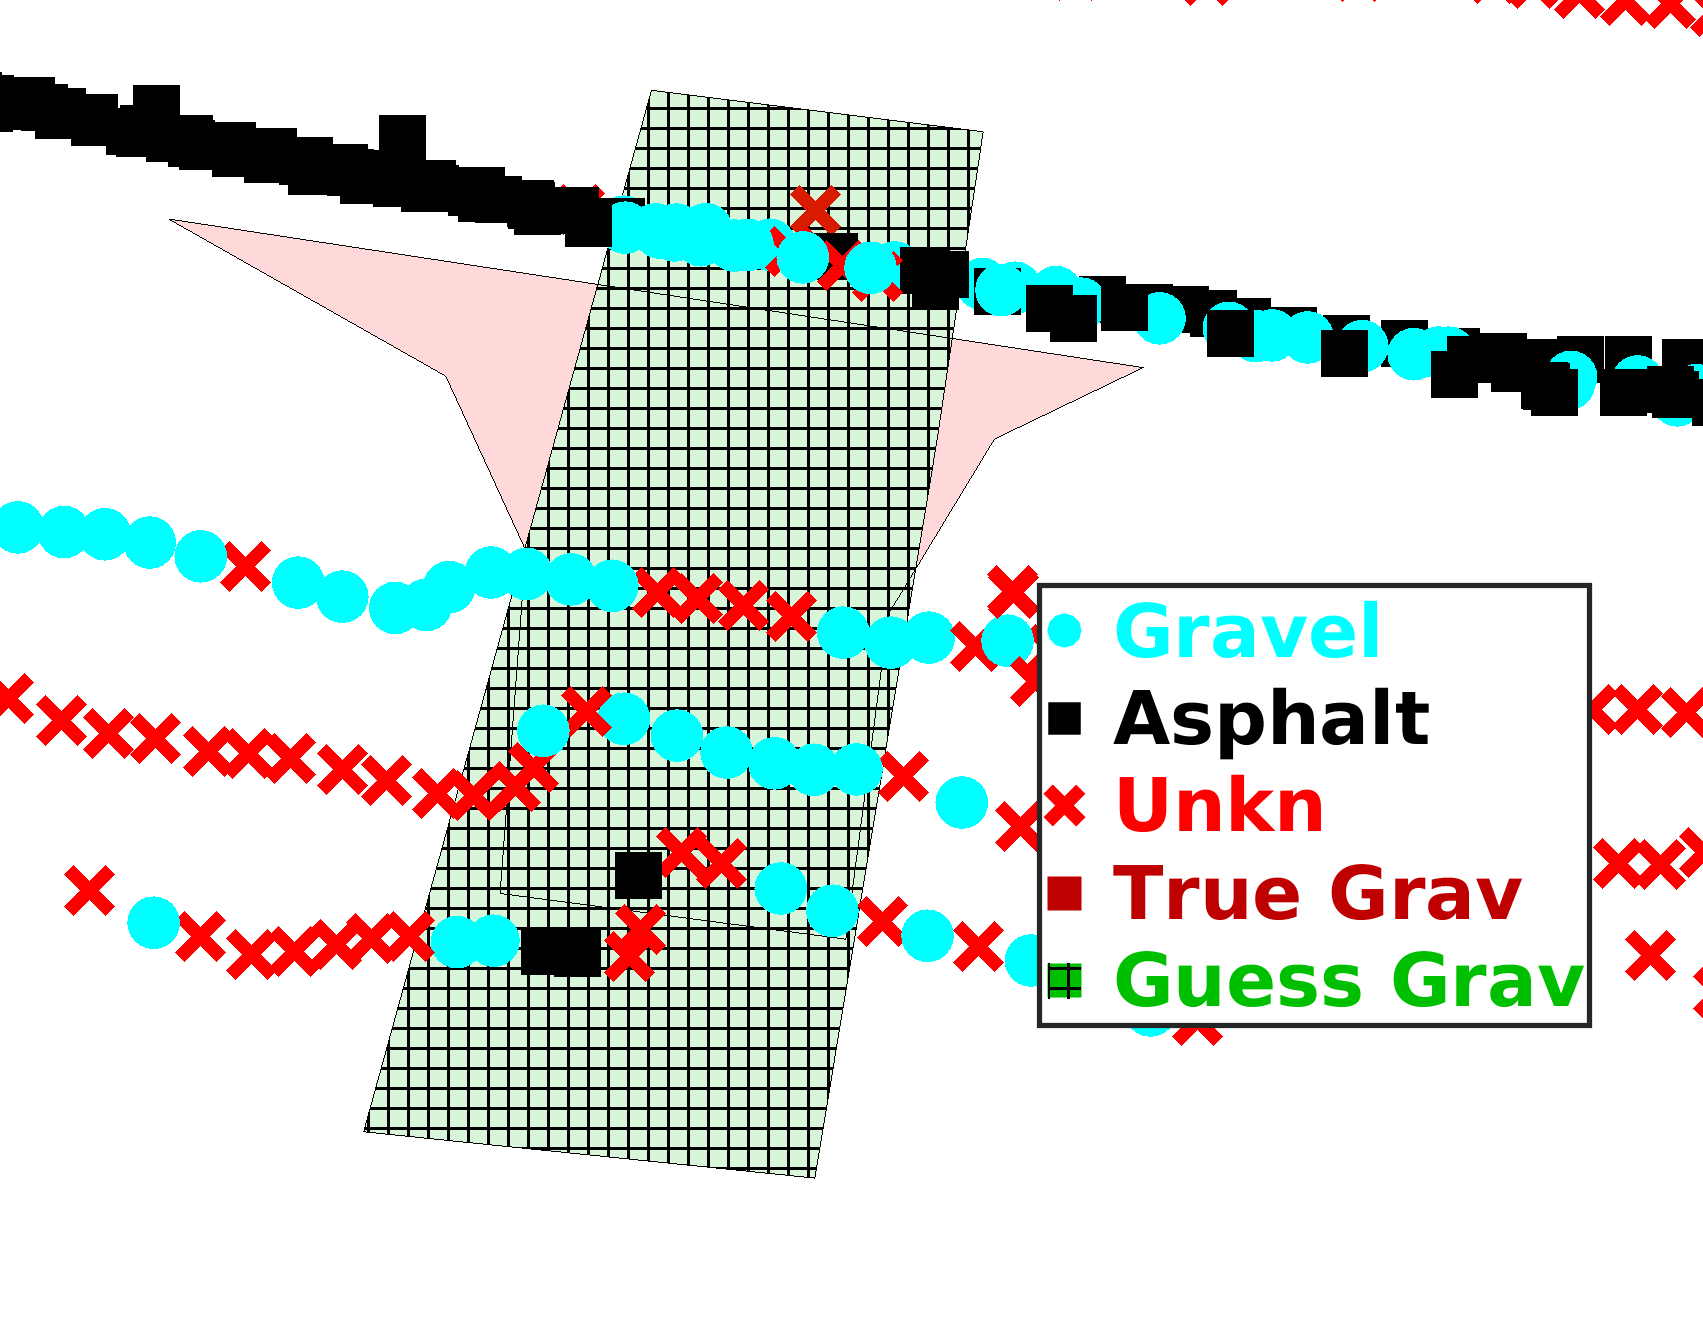
\includegraphics[width=0.9\linewidth]{Defense_Images/rm_db_6_overlap_2}
			\caption[Projected Visual Guess vs Truth]{Gravel surfaces were manually guessed and compared to actual gravel surface areas. Not shown is a similar method employed to compare guessed versus actual asphalt areas}
			\label{fig:rm_db_6_overlap_2}
		\end{figure}	

	}
	
	\section{Automated Road Detection}\label{sec:auto_road_detection}{
		
		{Automated detection of unmarked road was explored in order to determine if visual detection results may be repeated. Three areas were examined for classification trends across the three considered channels (Figure \ref{fig:auto_guess_areas}) in a post-processing step. Class percentages, standard deviation of height, standard deviation of average [x,y] distance to the LiDAR point of origin, and distance trends between classified arcs were exploited to determine if the area best describes a gravel, asphalt, or unknown surface (Figure \ref{fig:auto_guess_areas}). Results were compiled into a single classified map and compared to truth areas, then scored based off the number of true/false positive road detection (Figure \ref{fig:auto_guess_v_truth}).}	
		
		\begin{figure}[H]
			\centering
			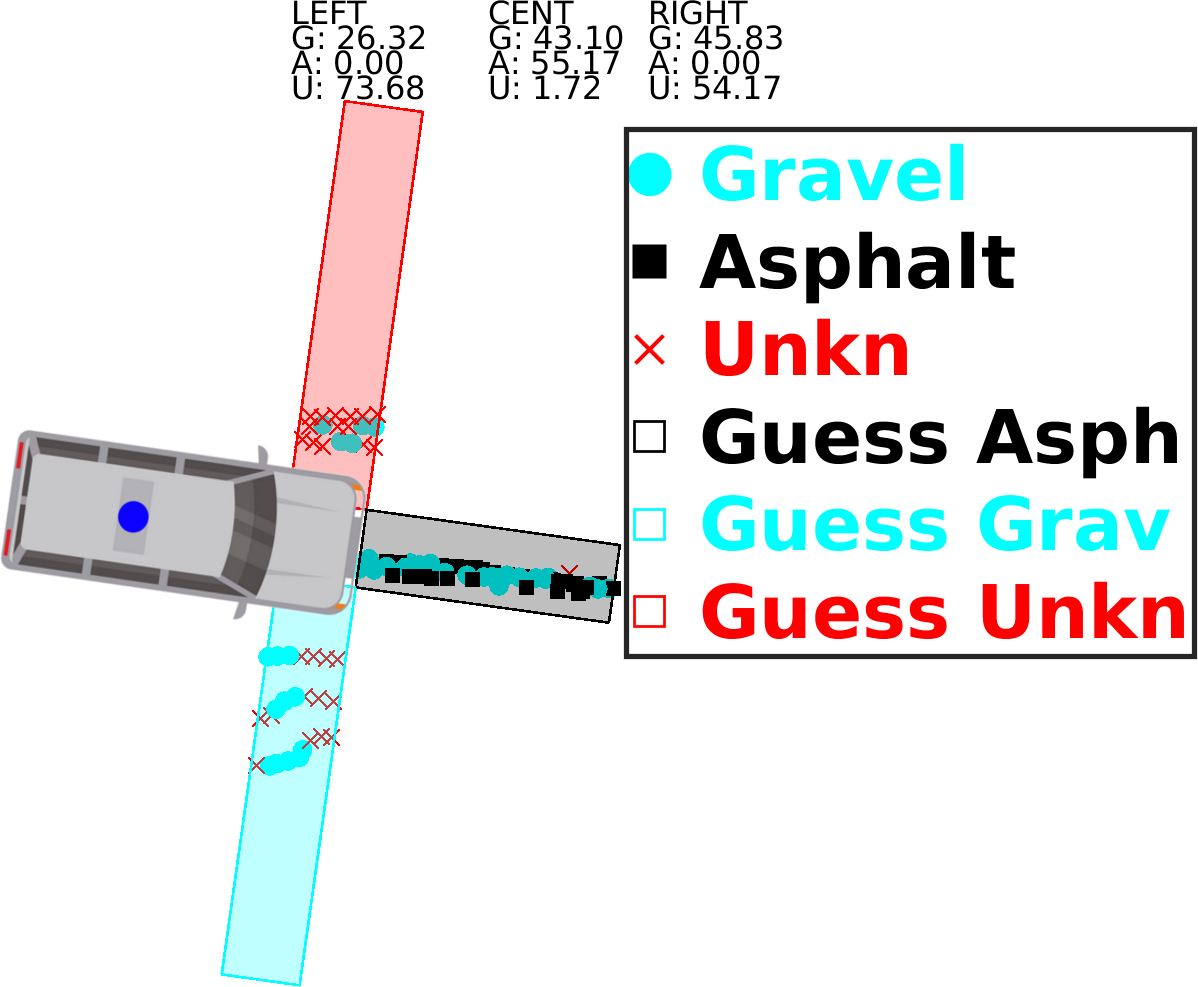
\includegraphics[width=0.9\linewidth]{Defense_Images/auto_area_guess}
			\caption[Projected Automated Guess vs Truth]{Automated detection of unmarked roads were explored for three areas (figure shows a top-down view) around the van. Trends across channels were examined, dictating the best guess for area class type. }
			\label{fig:auto_guess_areas}
		\end{figure}
		
		\begin{figure}[H]
			\centering
			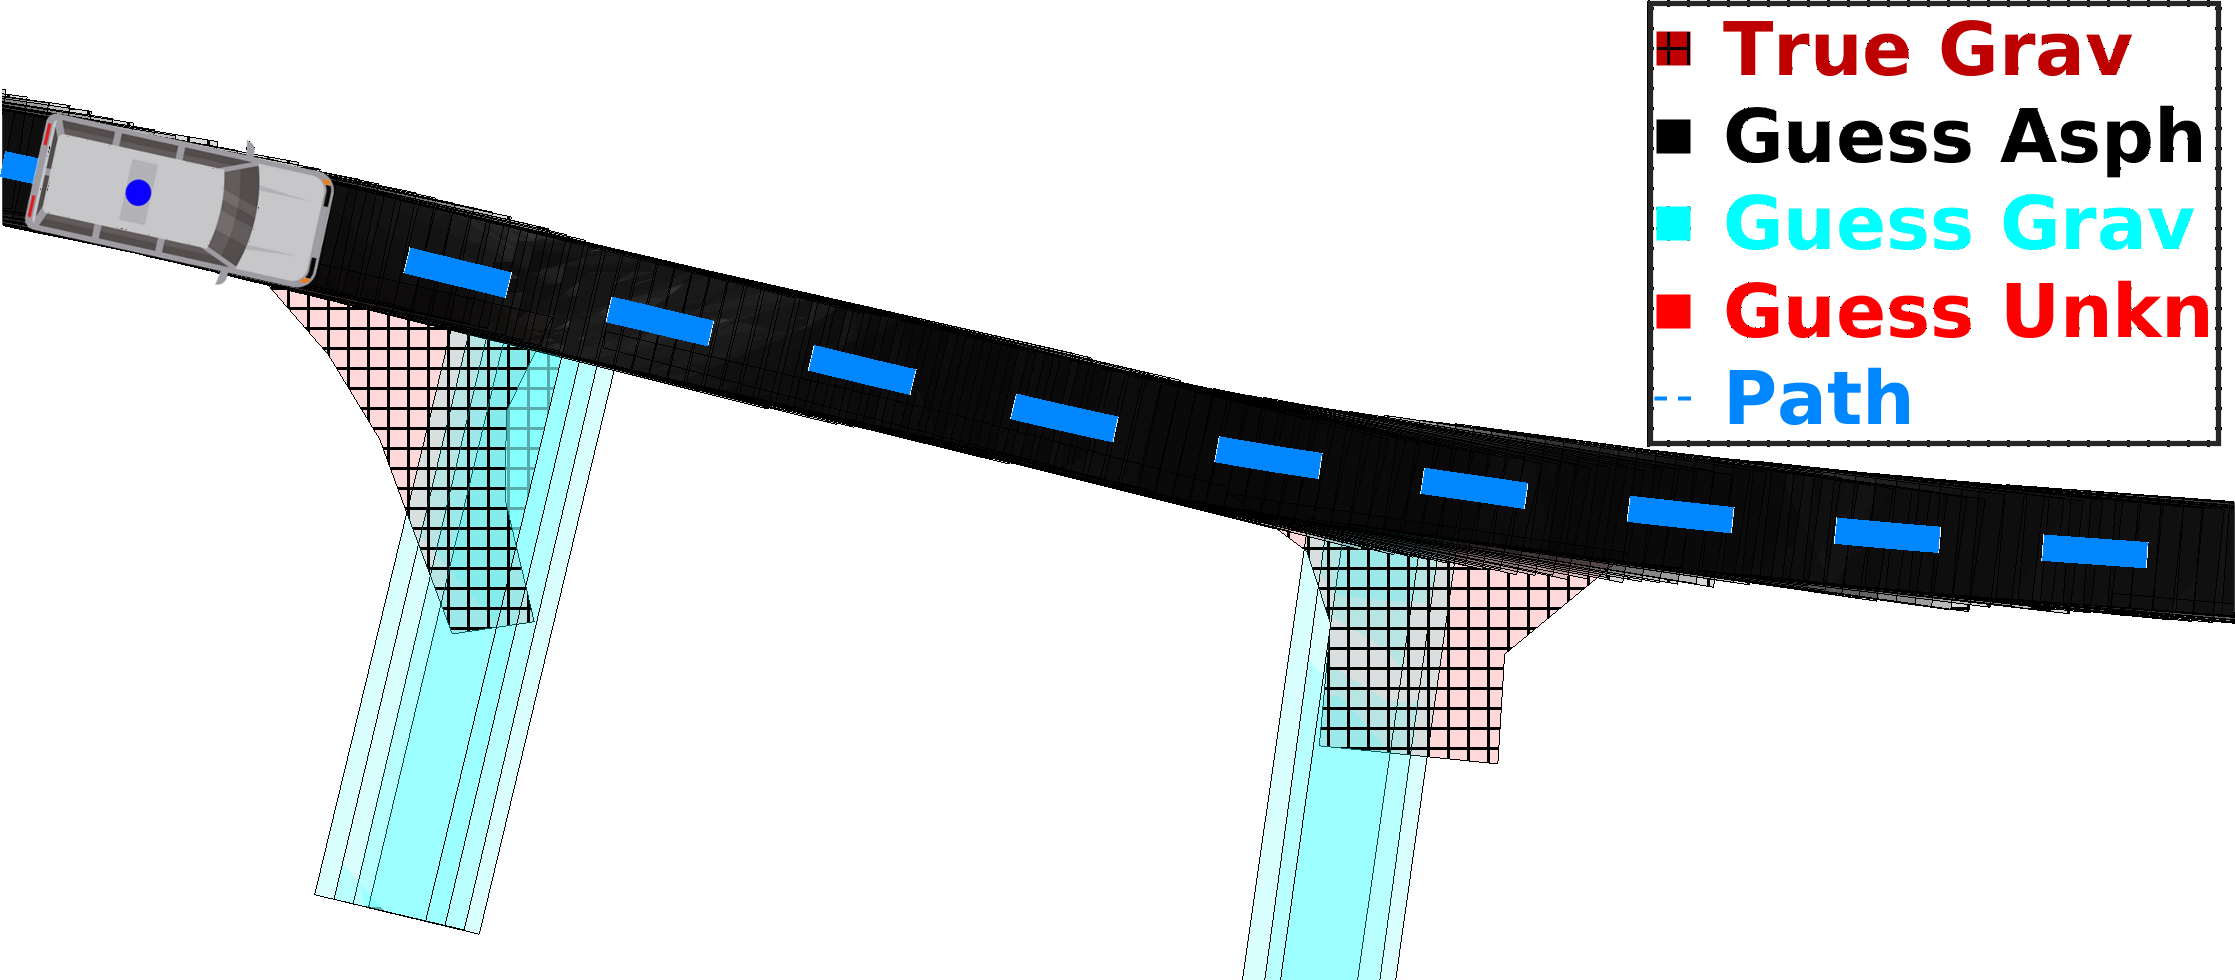
\includegraphics[width=0.9\linewidth]{Defense_Images/auto_guess_v_truth}
			\caption[Projected Automated Guess vs Truth]{Results of automated unmarked road detection were aggregated and compared to truth areas.}
			\label{fig:auto_guess_v_truth}
		\end{figure}	
		
	}
		
%		} % End Obj 2 Task 2

%	} % End Objective 2

\newpage
	
	
	\section{Summary of Methods}\label{sec:summary-of-methods}{
		
		{Detection of unmarked gravel road surfaces using terrain classification requires building a data base of terrain features, training an RDF, and testing the algorithm for accuracy of unmarked road detection. The experimental apparatus for this work will be the Ohio University Autonomous Van van. Scanning LiDAR, GPS, and IMU data will be gathered from a stretch of Blackburn Road that includes three intersecting gravel driveways. Point cloud data will be aggregated in order to create a single point cloud map. Manually defined 2D areas representing gravel and asphalt will be projected unto the point cloud. Training data will be extracted from the projected areas and used to train an RDF terrain classifier. Out-of-bag testing and validation accuracy will be used to verify the algorithms. Terrain classification of consecutive scans will be completed and scored by determining classified point distribution in each created truth area. Visual and automatic examination of class trends between channels allows for projection of best-guess road surfaces which will be subsequently compared to truth areas. \textbf{Final Deliverable:} Method of detecting a stretch of Blackburn Road that includes three intersecting gravel driveways by using a terrain classification algorithm to interpret scanning LiDAR data with the express purpose of predicting road surface area.}
		
	} % End Summary of Methods
	
} % End Methodolgy

\chapter{Results}{
	
	\section{Training Data Collection}\label{sec:training-data-collection}{
		
		\begin{figure}[H]
			\centering
			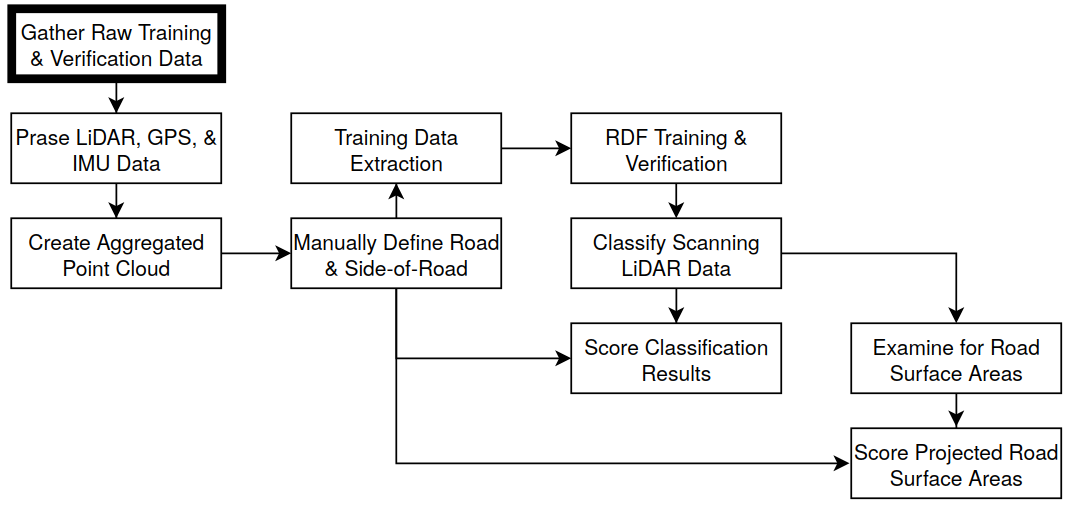
\includegraphics[width=0.9\linewidth]{Defense_Images/flowz_gather_data}
			\caption[Training Data Collection Flowchart Context]{The following section addresses the gathering of training data.}
			\label{fig:flowz_gather_data}
		\end{figure}
	
		{Training and verification LiDAR, GPS, and IMU data collection was completed using the Experimental Apparatus (Figure \ref{fig:Experimental_Apperatus_in_Results}). Gravel data was gathered from the Redmen Lodge gravel parking lot, while grass data was gathered beside the lot (Figure \ref{fig:gravel_training_lot}). Three gravel driveways intercept Blackburn Road (Figure \ref{fig:road_areas_annotated_2}; Figures \ref{fig:training_gravel}, \ref{fig:driveway_2}, and \ref{fig:driveway_1} show example gravel from driveways 3, 2, and 1 respectively). Asphalt data was gathered Blackburn Road (Figure \ref{fig:Blackburn_Road_View}). It was later found that certain areas by the side of the road (Figure \ref{fig:here_be_dirt}, \ref{fig:here_be_side_of_road_dirt}) were difficult to classify due to feature overlap (Section \ref{sec:training_data_extraction}). }
			
%			Point cloud data from the resulting rosbags was manually defined by area as one of three terrain types: gravel, chipseal, or grass. 
%			Training data was extracted from designated areas that were seperate from the testing areas (Figure \ref{fig:test_vs_train_areas}). 
%			Although this work does not evaluate the detection accuracy of grass, differentiation between a road and non-road surface is necessary for evaluating road-surface detection, therefore grass is labeled as \textit{unknown} in this work.} 
%		
		\begin{figure}[H]
			\centering
			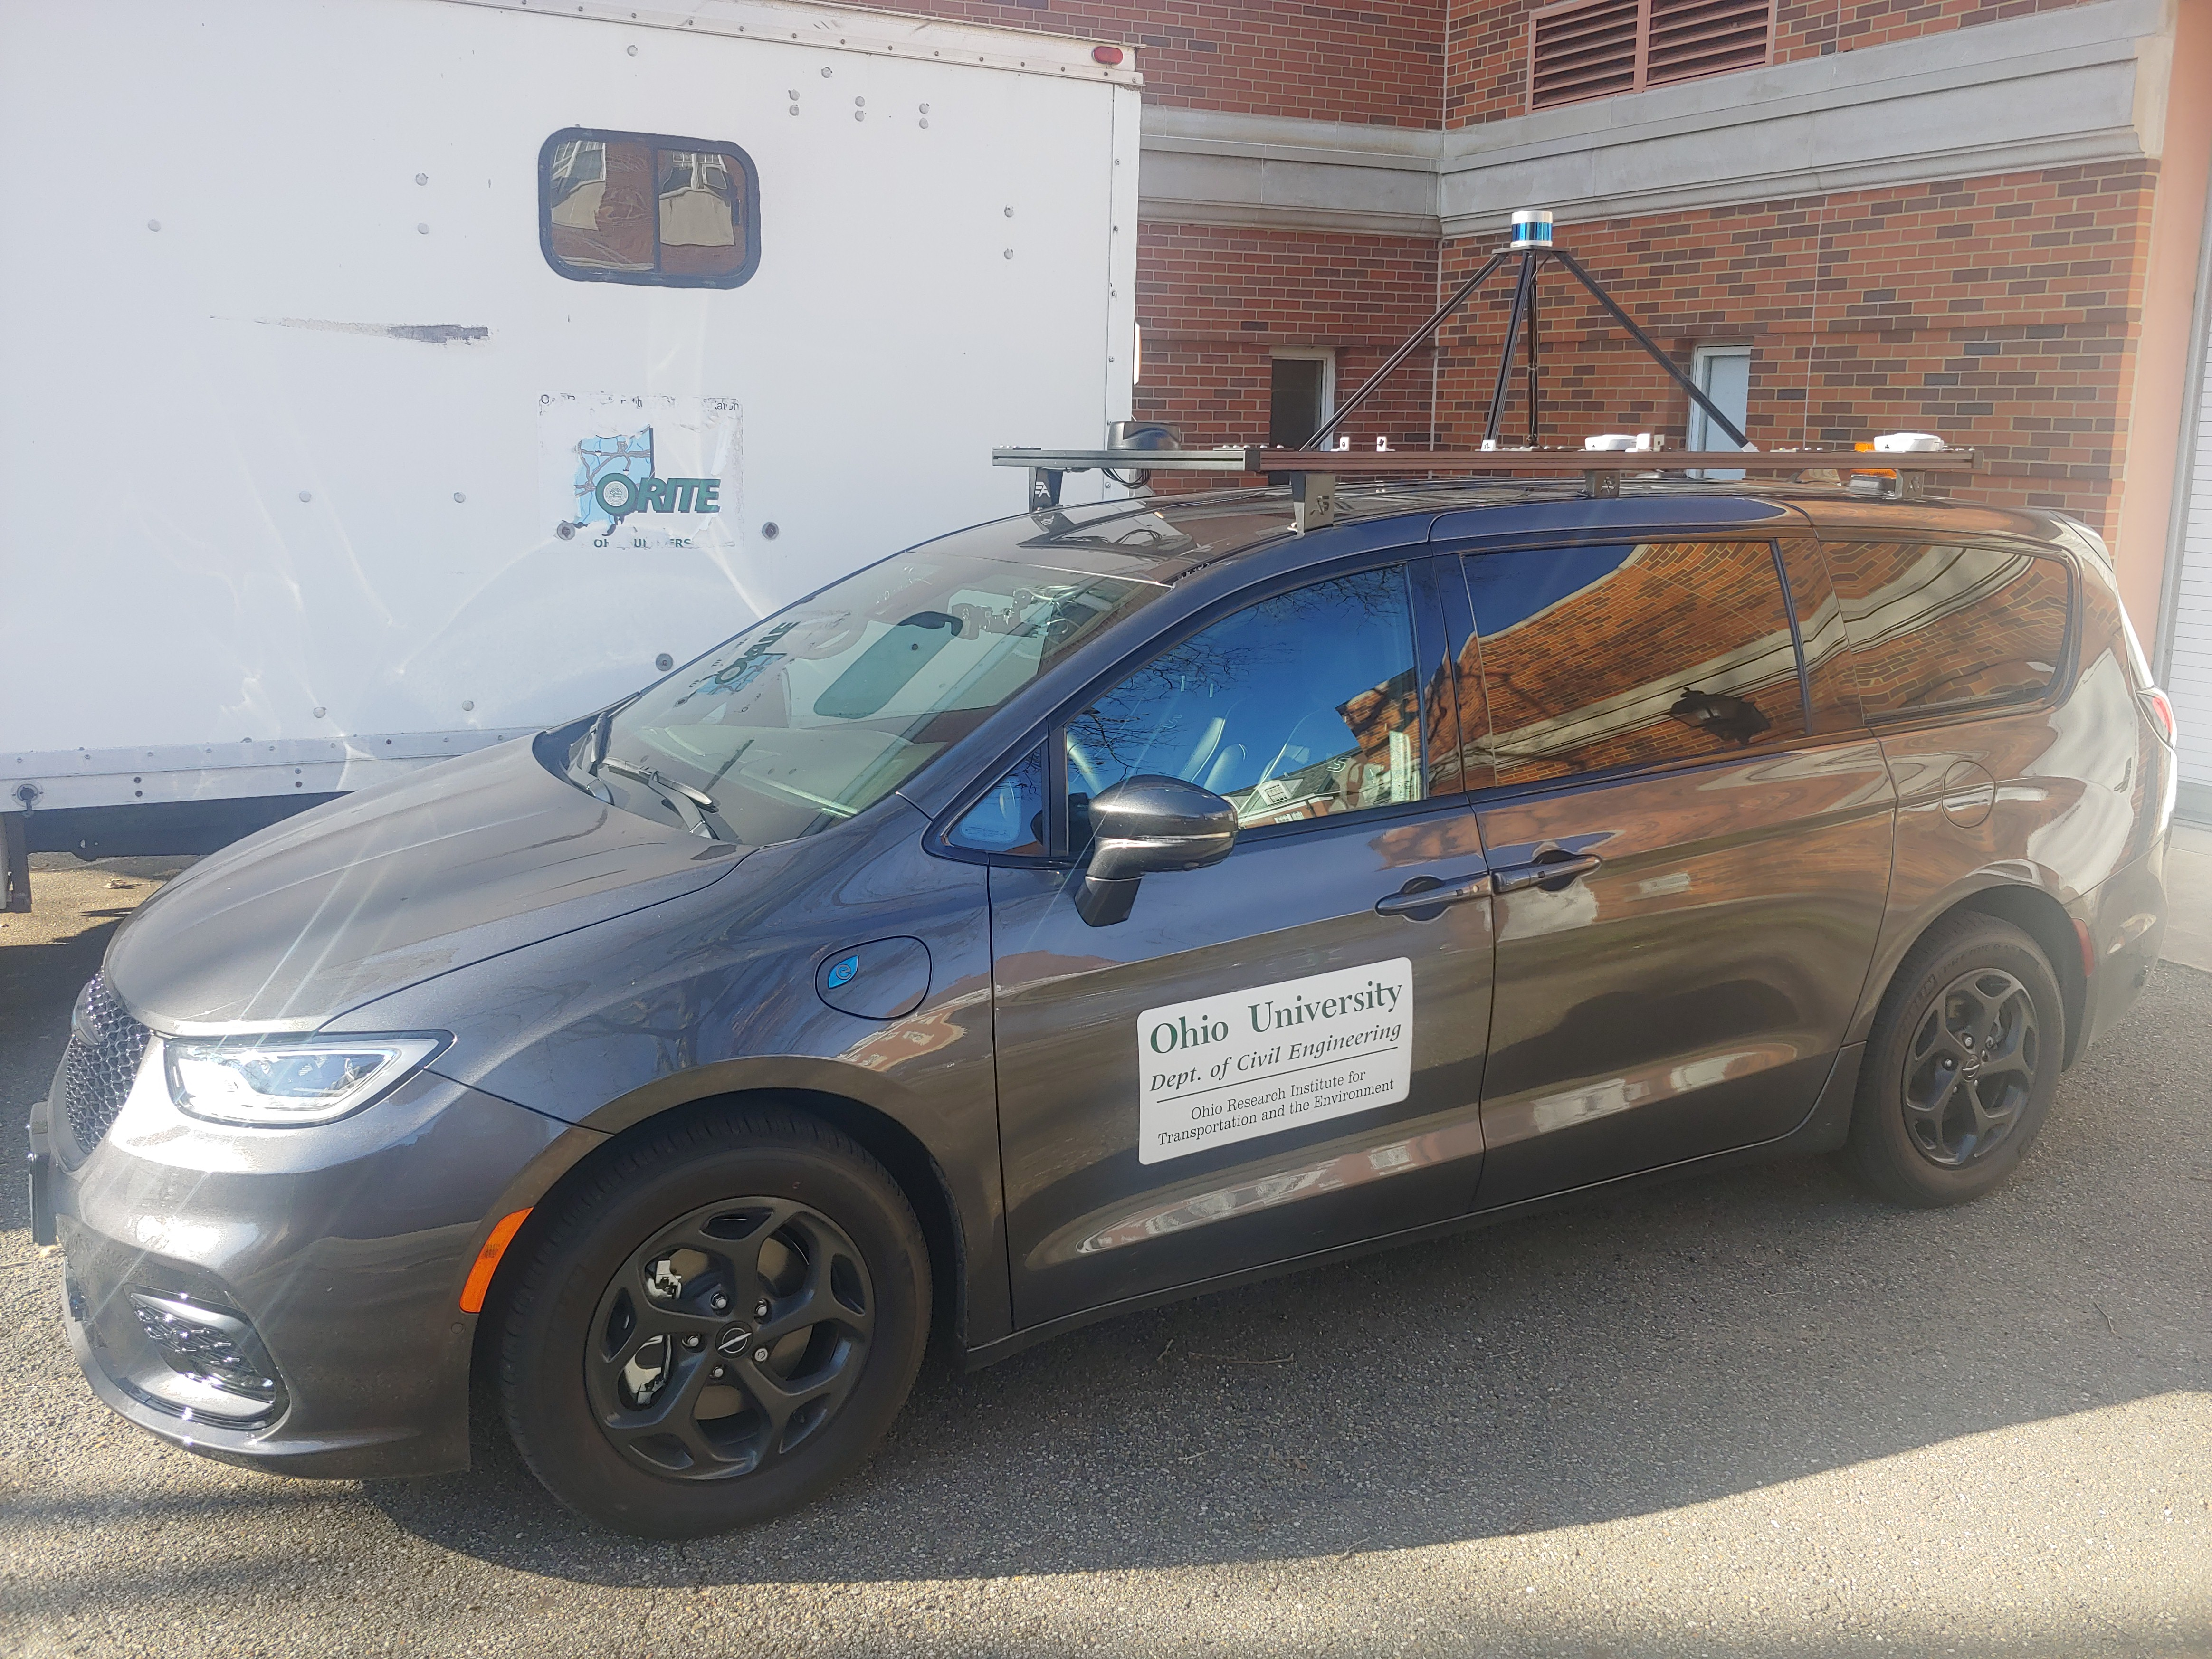
\includegraphics[width=0.7\linewidth]{Defense_Images/van_on_van}
			\caption[Sensor Van]{Sensor Van built by AutonomouStuff}
			\label{fig:Experimental_Apperatus_in_Results}
		\end{figure}
		
		\begin{figure}[H]
			\centering
			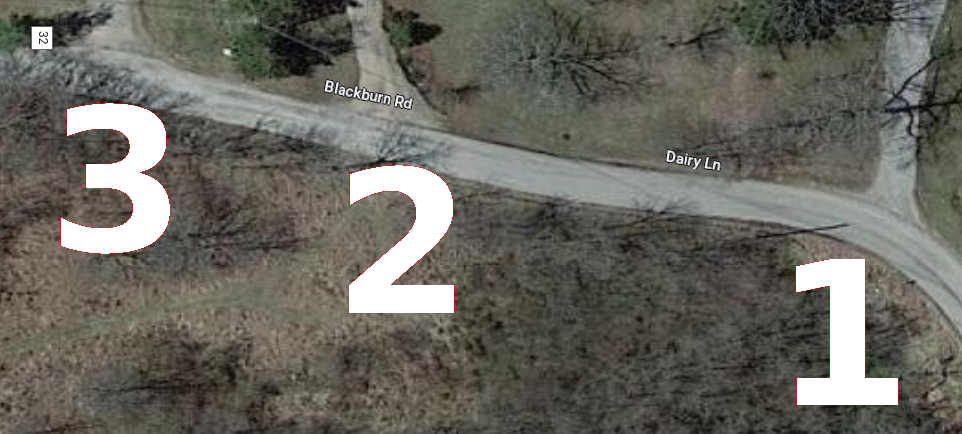
\includegraphics[width=0.65\linewidth]{Defense_Images/three_driveways_sat}
			\caption[Blackburn Road Overlays]{Blackburn Road with three intercepting driveways. Driveway $3$ is the entrance to the lot from which gravel training data was gathered. }
			\label{fig:road_areas_annotated_2}
		\end{figure}
		
		\begin{figure}[H]
			\centering
			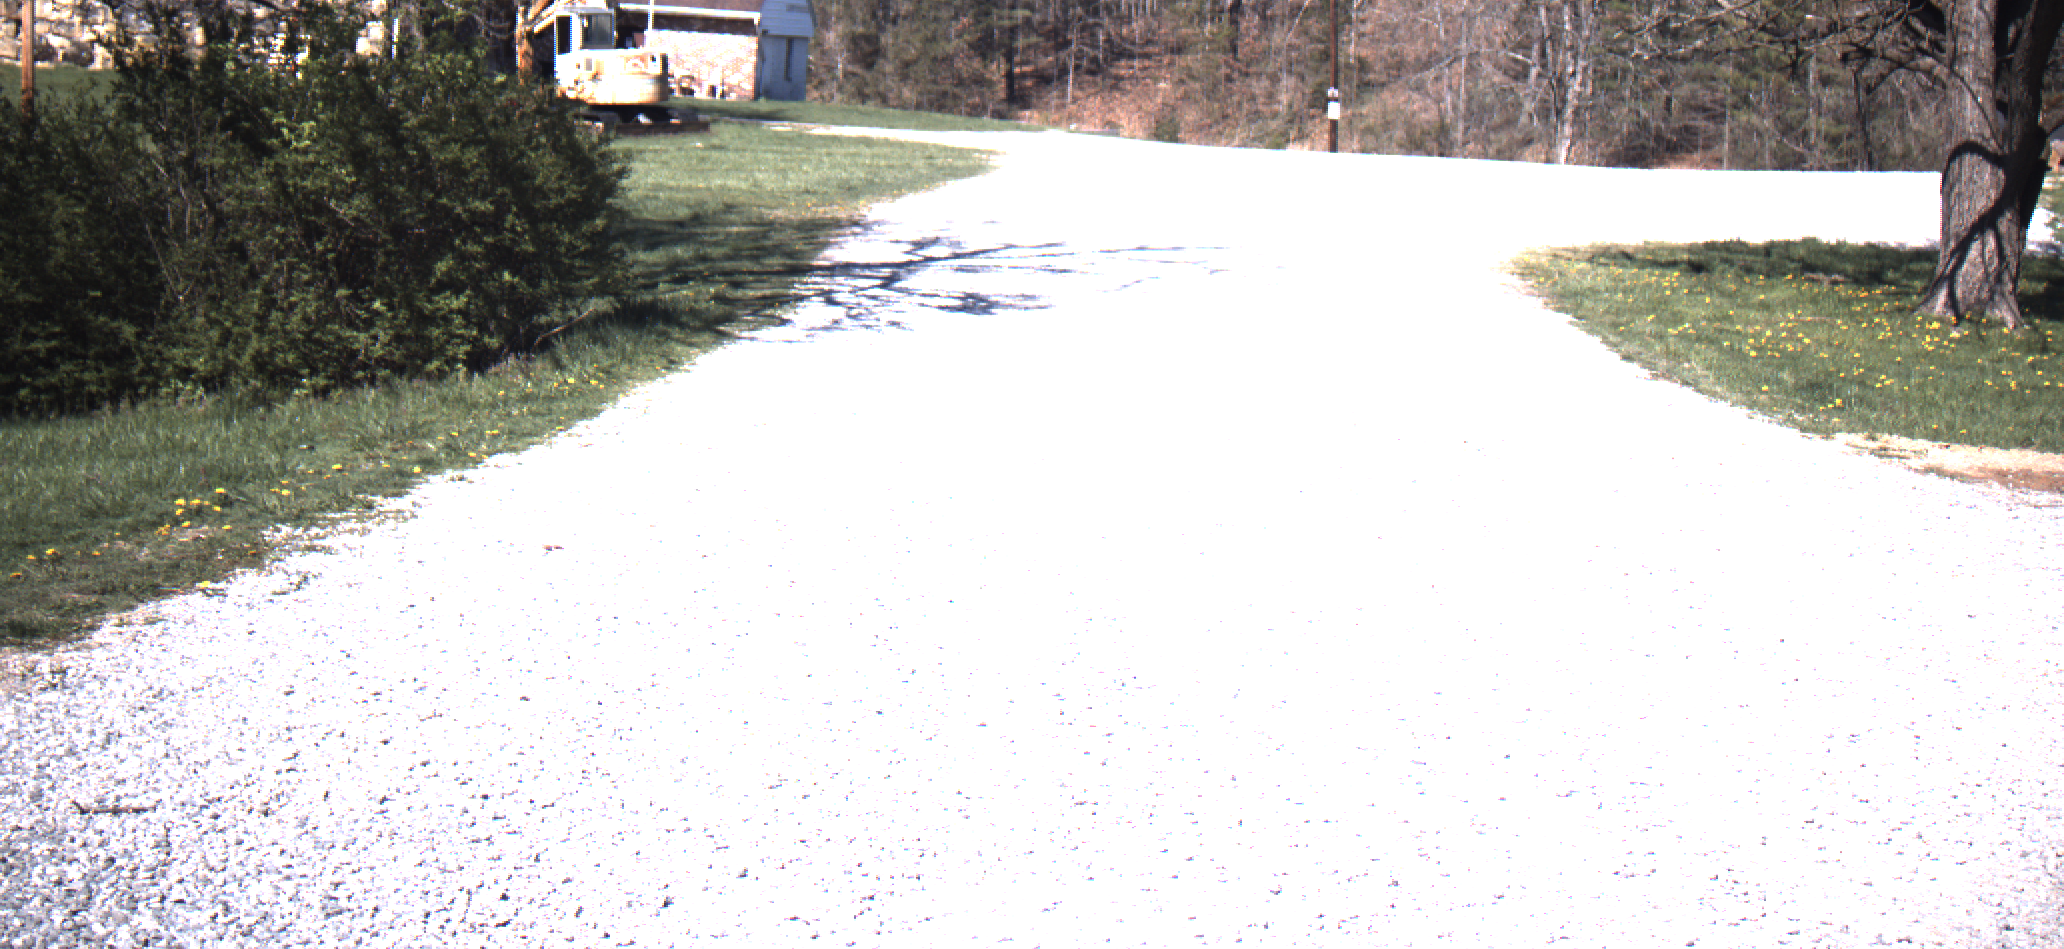
\includegraphics[width=0.75\linewidth]{Defense_Images/gravel_training_lot}
			\caption[Gravel Training Lot]{Camera view of the gravel lot from which gravel training data was gathered.}
			\label{fig:gravel_training_lot_in_results}
		\end{figure}

		\begin{figure}[H]
			\centering
			\includegraphics[width=0.75\linewidth]{Defense_Images/training_gravel}
			\caption[Training Gravel]{Close-up of gravel that makes up the training lot (driveway 3).}
			\label{fig:training_gravel}
		\end{figure}
		
		\begin{figure}[H]
			\centering
			\includegraphics[width=0.75\linewidth]{Defense_Images/driveway_2}
			\caption[Driveway 2 Gravel]{Close-up of gravel from driveway 2.}
			\label{fig:driveway_2}
		\end{figure}
		
		\begin{figure}[H]
			\centering
			\includegraphics[width=0.75\linewidth]{Defense_Images/driveway_1}
			\caption[Driveway 2 Gravel]{Close-up of gravel from driveway 1.}
			\label{fig:driveway_1}
		\end{figure}
		
		\begin{figure}[H]
			\centering
			\includegraphics[width=0.75\linewidth]{Defense_Images/vlcsnap-2023-04-20-08h48m17s447}
			\caption[Blackburn Road Camera View]{Camera view of Blackburn Road - an unmarked asphalt road with three intercepting gravel driveways from which asphalt data was gathered.}
			\label{fig:Blackburn_Road_View_in_results}
		\end{figure}
			
		\begin{figure}[H]
			\centering
			\includegraphics[width=0.65\linewidth]{Defense_Images/here_be_dirt}
			\caption[Re-grassed Dirt]{Dirt being re-grassed leads to terrain classification confusion with gravel surfaces.}
			\label{fig:here_be_dirt}
		\end{figure}
				
		\begin{figure}[H]
			\centering
			\includegraphics[width=0.65\linewidth]{Defense_Images/here_be_side_of_road_dirt}
			\caption[Dirt on Side of Road]{Dirt on side of road in this configuration was found to cause terrain classification confusion with gravel surfaces.}
			\label{fig:here_be_side_of_road_dirt}
		\end{figure}

		

		
	} % Training Data Collection
	
	\section{Parse Raw Training Data}\label{sec:parse_raw_training_data}{
		
		\begin{figure}[H]
			\centering
			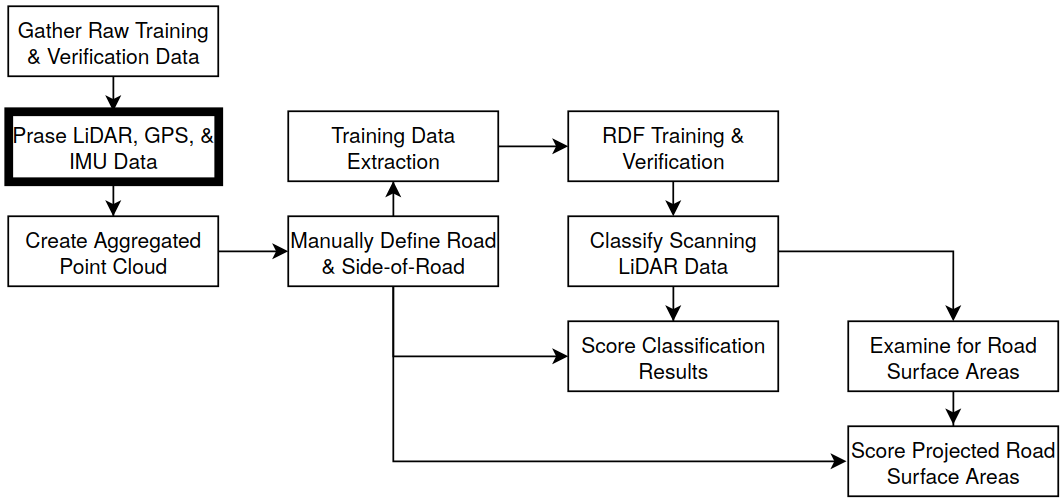
\includegraphics[width=0.9\linewidth]{Defense_Images/flowz_parse_data}
			\caption[Training Data Parsing Flowchart Context]{The following section addresses the parsing gathered raw data.}
			\label{fig:flowz_parse_data}
		\end{figure}
		
		{MATLAB was used to parse rosbag files containing the scanning LiDAR, GPS, and IMU data into separate data streams. LiDAR data is extracted as an array of 3d points with associated intensity and channel information (Figure \ref{fig:pcd_example}, Table \ref{tab:example_lidar_data}). GPS data is extracted as a table containing longitude and latitude (Table \ref{tab:example_gps_data}). IMU data is extracted as a table containing roll, pitch, and yaw (Table \ref{tab:example_imu_data}).}
		
		% HOW did I extract data
		
		% What does the extracted data look like?
		
		% Need: example gps/imu table, example single-scan of point cloud
		\begin{figure}[H]
			\centering
			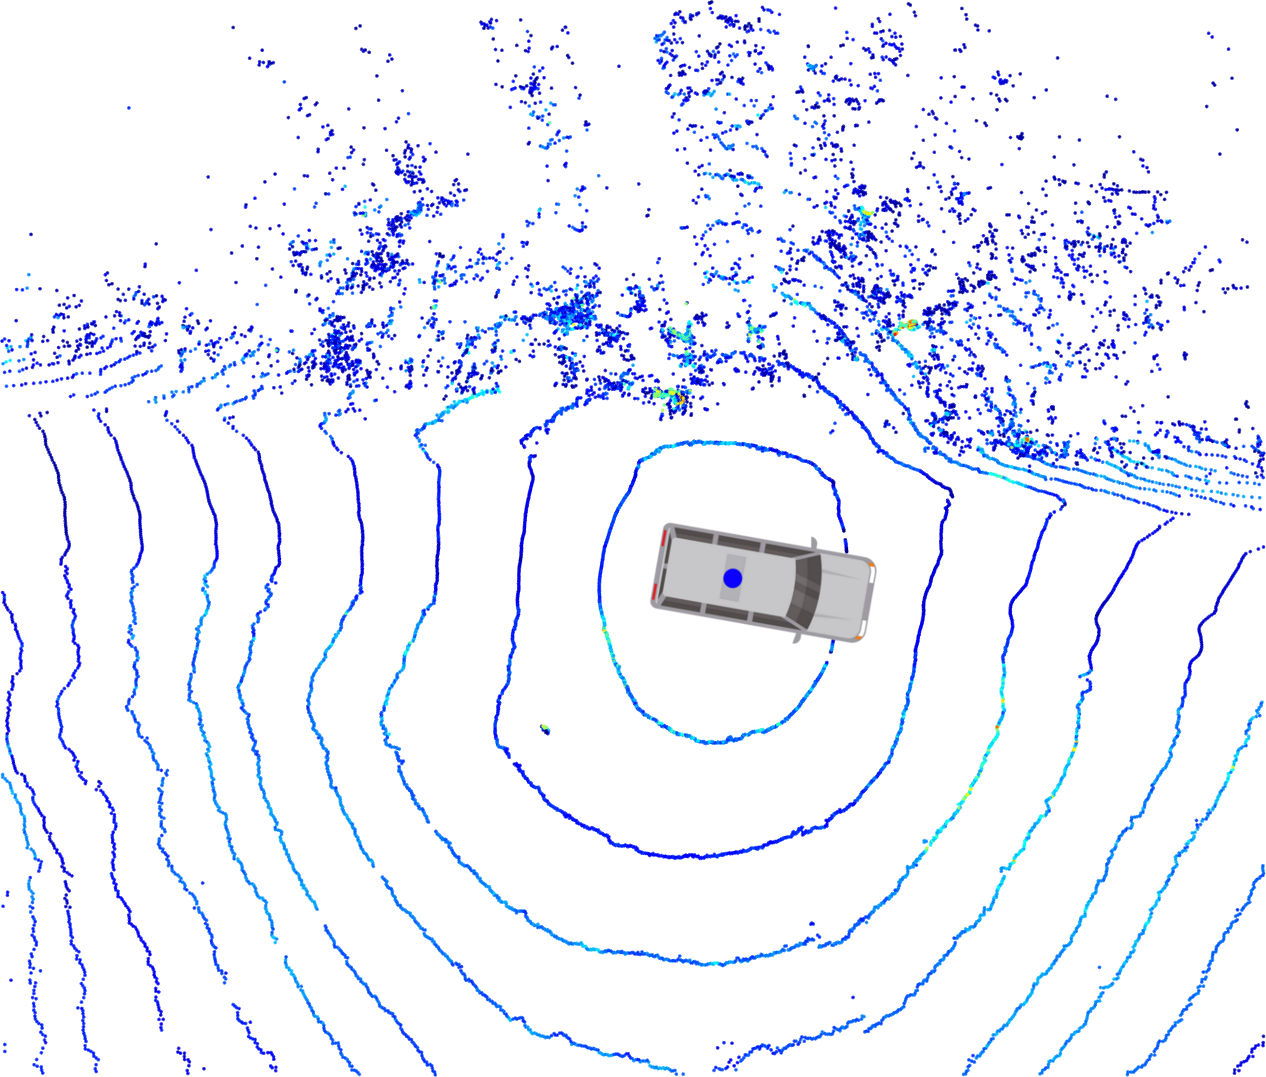
\includegraphics[width=0.95\linewidth]{Defense_Images/pcd_example_with_van}
			\caption[Example Point Cloud]{Top-down view of an example 3D point cloud with the van indicating LiDAR position as the blue dot. Differences in perceived intensities dictates point color in this image.}
			\label{fig:pcd_example}
		\end{figure}
		
		\begin{table}[H]
			\centering
			\begin{tabular}{|c|c|c|c|c|}
				\hline
				x (m)     & y (m)      & z (m)      & i   & ring \\
				\hline
				2.0269465 & -5.8238673 & -2.875495  & 44  & 0    \\
				\hline
				2.006604  & -5.8309078 & -2.875495  & 33  & 0    \\
				\hline
				1.9850709 & -5.8344445 & -2.8738043 & 36  & 0    \\
				\hline
				1.9680247 & -5.8478665 & -2.8771851 & 33  & 0    \\
				\hline
				...       & ...        & ...        & ... & ...  \\
				\hline
			\end{tabular}
			\caption[Example LiDAR Data]{Example of LiDAR data. While position \textit{(x, y, and z)} units are in meters, intensity \textit{(i)} is a unit-less ratio between minimum and maximum detectable intensity \textit{(0-255)}. \textit{Ring} references one of the VLP-32C's channels \textit{(0-31)}.}
			\label{tab:example_lidar_data}
		\end{table}
		
		\begin{table}[H]
			\centering
			\begin{tabular}{|c|c|c|}
				\hline
				Lat (deg)   & Lon (deg)    & Alt (m)     \\
				\hline
				39.31384707 & -82.12226358 & 236.7873663 \\
				\hline
				39.31384022 & -82.12226475 & 236.8764364 \\
				\hline
				39.3138334  & -82.12226598 & 236.970671  \\
				\hline
				39.31382661 & -82.12226723 & 237.0683338 \\
				\hline
				...         & ...          & ...       \\ 
				\hline
			\end{tabular}
			\caption[Example GPS Data]{Example of GPS data. }
			\label{tab:example_gps_data}
		\end{table}	
	
		
		\begin{table}[H]
		\centering
		\begin{tabular}{|c|c|c|}
			\hline
			Roll (deg)  & Pitch (deg)  & Yaw (deg)   \\
			\hline
			0.331466984 & -7.267827997 & 82.86123384 \\
			\hline
			0.66596557  & -7.39710978  & 82.38362661 \\
			\hline
			0.891057082 & -7.388438597 & 82.04084302 \\
			\hline
			0.833872274 & -7.294207298 & 82.09796229 \\
			\hline
			...         & ...          & ...        \\
			\hline
		\end{tabular}
		\caption[Example IMU Data]{Example of IMU data.}
		\label{tab:example_imu_data}
		\end{table}
		
		
	} % Parse Raw Training Data
	
	\section{Creating Aggregated Point Cloud}\label{sec:create_aggregated_point_cloud}{
		
		\begin{figure}[H]
			\centering
			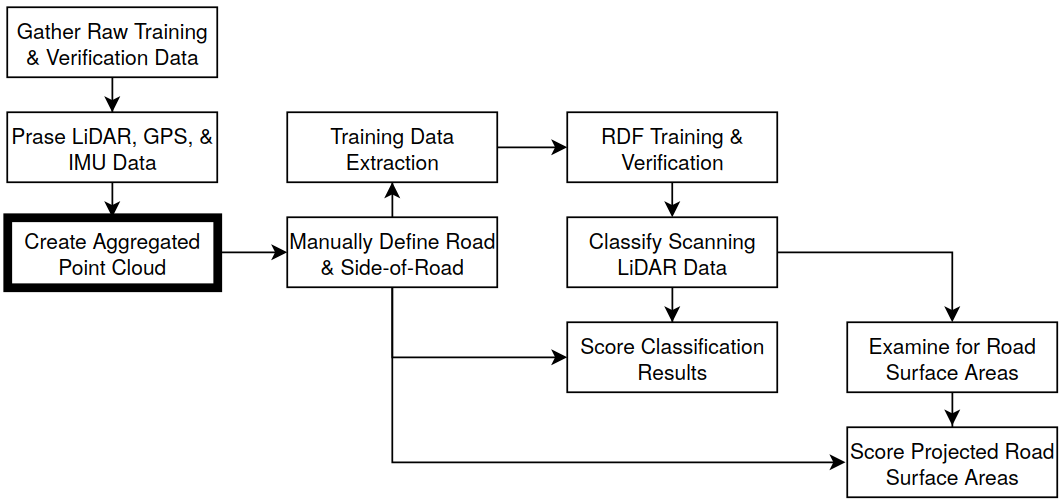
\includegraphics[width=0.9\linewidth]{Defense_Images/flowz_point_cloud}
			\caption[Aggregating Point Cloud Data Flowchart Context]{The following section addresses compiling single LiDAR scans into an aggregated point cloud.}
			\label{fig:flowz_point_cloud}
		\end{figure}
		
		{Extracting training data from single LiDAR scans such as in Figure \ref{fig:pcd_example} is extremely time consuming as potentially thousands of scans must be manually examined, therefore it was deemed necessary to pull training data from aggregated point clouds to expedite the process. Scanning LiDAR timestamps were matched to the closest GNSS and IMU timestamp data. Closest matching GNSS and IMU data informed the location and orientation of the LiDAR scan. Point cloud translation and rotation was accomplished using transformation matrices derived from GPS and IMU data. Rotation matrices were created using extracted roll, pitch, and yaw data from the IMU. LiDAR origin was found using GPS longitude, latitude, and altitude data. Physical distances between the GPS, IMU, and LiDAR sensors was rectified by obtaining reference frames provided by AutonomouStuff. GPS coordinates were offset by the current orientation and converted the ground truth to the LiDAR frame. GPS, IMU, and LiDAR reference frames and rotational updates were combined into trajectory vectors. Transformation matrices were then derived using MATLAB's $rigid3d$ function. Consecutive point cloud scans may then translated and rotated with derived transformation matrices (Fig. \ref{fig:combined_pcd_example}, \ref{fig:combined_gravel_pcd_example}). Each rosbag was processed to create a combined point cloud for the purpose of designating training and testing areas.}
		
		\begin{figure}[H]
			\centering
			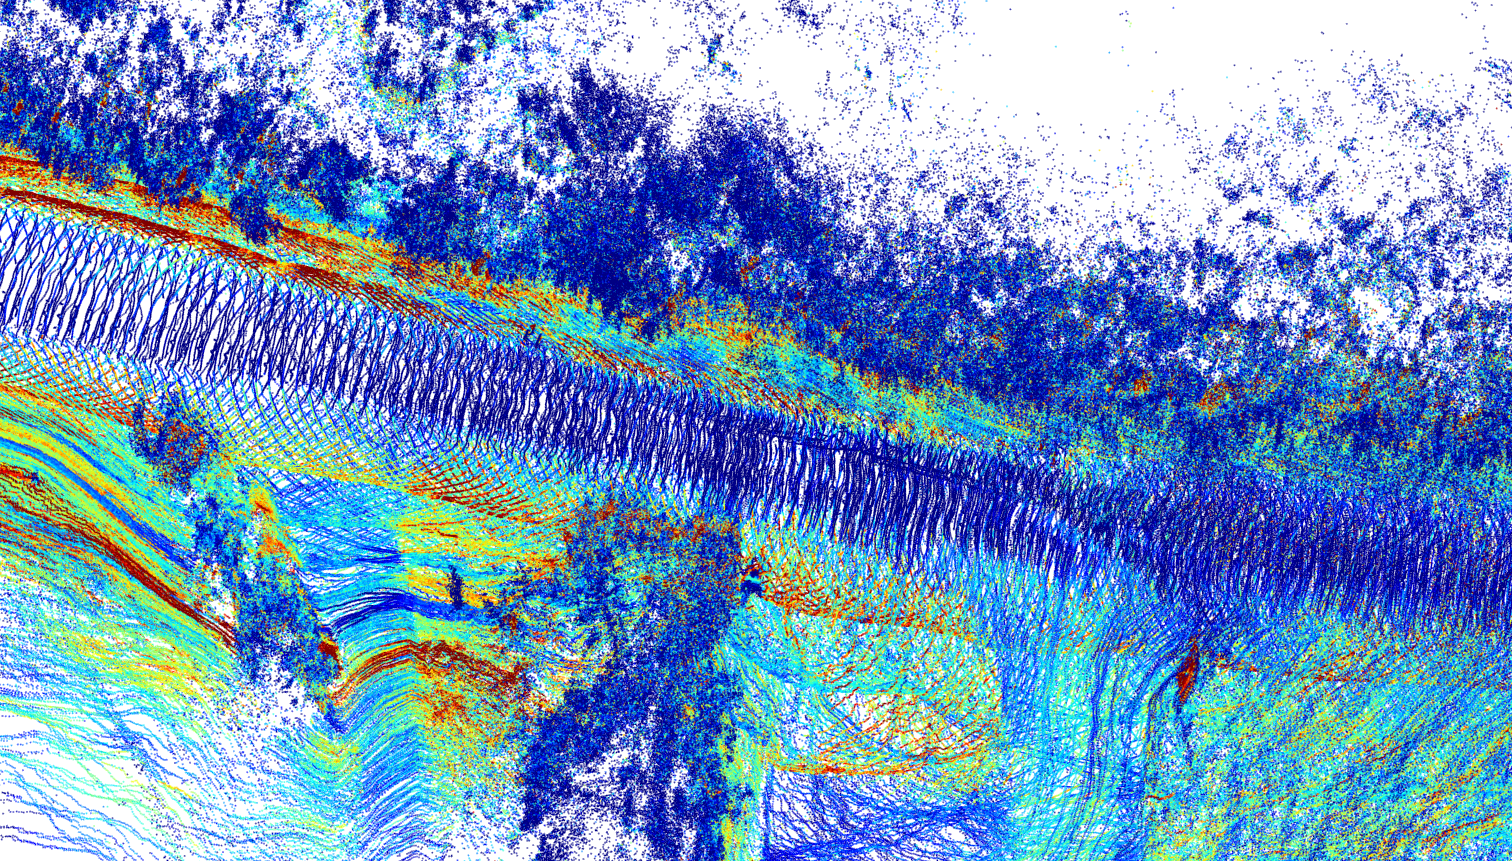
\includegraphics[width=0.95\linewidth]{Defense_Images/combined_pcd_example}
			\caption[Example Aggregated Point Cloud]{Example of aggregated point cloud data from Blackburn Road.}
			\label{fig:combined_pcd_example}
		\end{figure}
		
		\begin{figure}[H]
			\centering
			\includegraphics[width=0.95\linewidth]{Defense_Images/combined_gravel_pcd_example}
			\caption[Example Aggregated Point Cloud]{Example of aggregated point cloud data from the gravel lot and the neighboring grassy lawn.}
			\label{fig:combined_gravel_pcd_example}
		\end{figure}	
			
	} % Creating Aggregated Point Cloud
	
	\section{Manually Defining Areas}\label{sec:manually_defining_areas}{
		
		\begin{figure}[H]
			\centering
			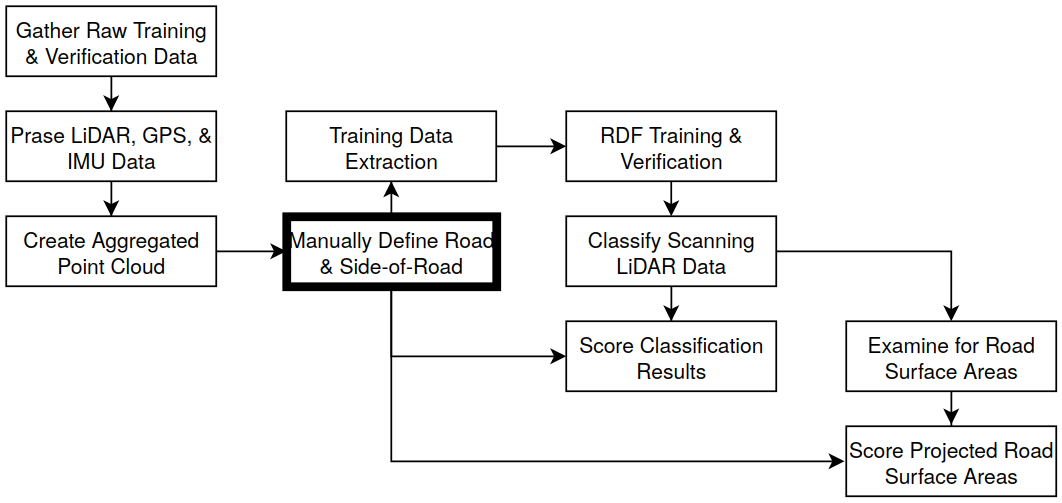
\includegraphics[width=0.9\linewidth]{Defense_Images/flowz_define_areas}
			\caption[Manually Defined Areas Flowchart Context]{The following section addresses the process of selecting training and testing areas from an aggregated point cloud.}
			\label{fig:flowz_define_areas}
		\end{figure}
		
		{MATLAB was used to visually examine aggregated point cloud data in order to project manually defined areas representing training and testing areas. After loading an aggregated point cloud into MATLAB's environment, the built-in $drawpolygon$ function is used to define \textit{gravel}, \textit{asphalt}, and \textit{unknown} areas. 2D Areas are selected from a top-down view of the aggregated point cloud, allowing future processes to compare a point's x and y coordinates. While a 3D area may be used, it was found that a 2D area was sufficient for this work. All rosbags were processed in this manner to define \textit{gravel}, \textit{asphalt}, and \textit{unknown} training and testing areas (Figure \ref{fig:test_vs_train_areas_in_results}).}
		
		% HOW did I define road areas
		
		\begin{figure}[H]
			\centering
			\begin{subfigure}{0.45\textwidth}
				\centering
				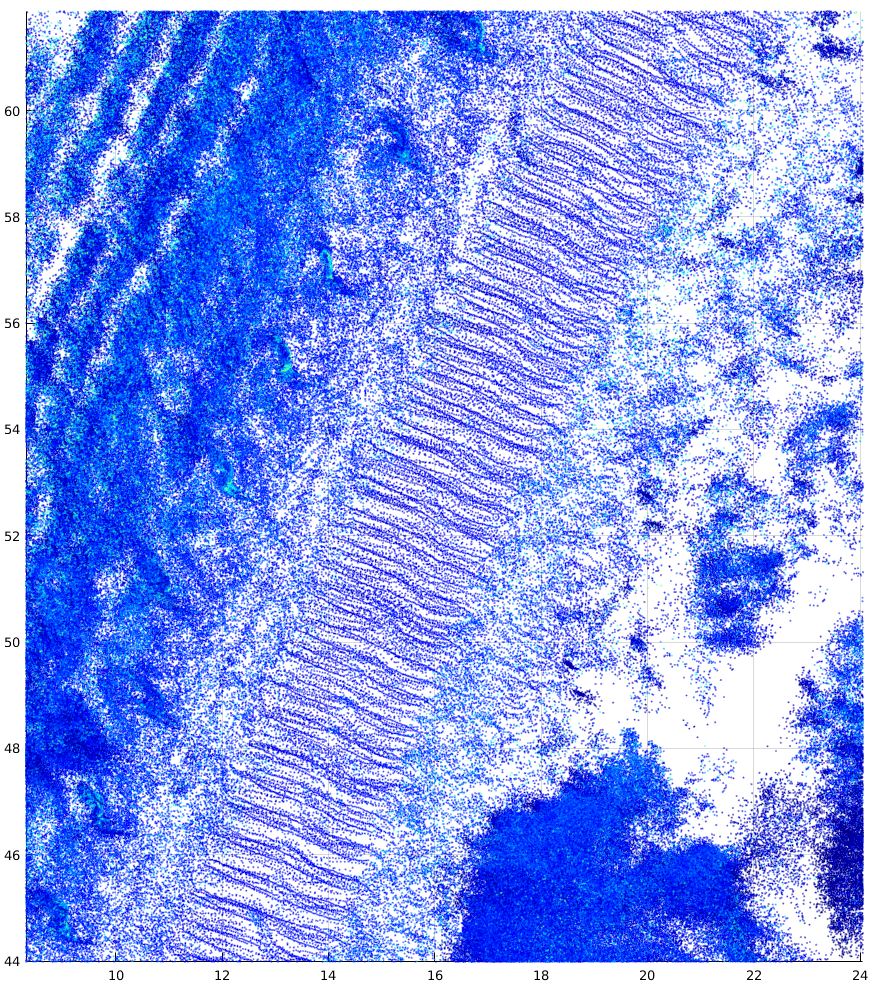
\includegraphics[width=1.0\linewidth]{Defense_Images/pre_select_area}
				\caption[Road area on Point Cloud]{}
				\label{fig:pre_select_area_in_results}
			\end{subfigure}
			\begin{subfigure}{0.45\textwidth}
				\centering
				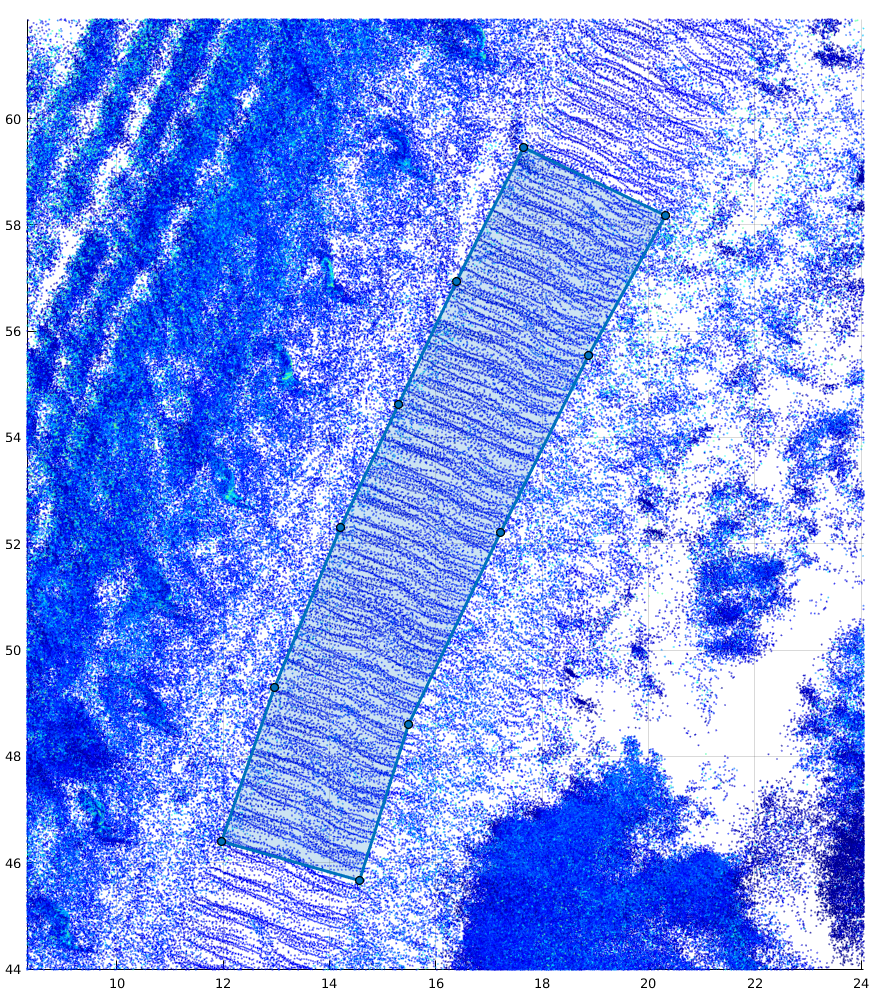
\includegraphics[width=1.0\linewidth]{Defense_Images/area_selected}
				\caption[Selected Road area on Point Cloud]{}
				\label{fig:area_selected_in_results}
			\end{subfigure}
			\caption[Manual Area Selection Process]{Combined scanning LiDAR point cloud data (a) may be manually defined using MATLAB's $drawpolygon$ function to select the desired area (b). }
			\label{fig:Area_Selection_Process_in_results}
		\end{figure}
		
		\begin{figure}[H]
			\centering
			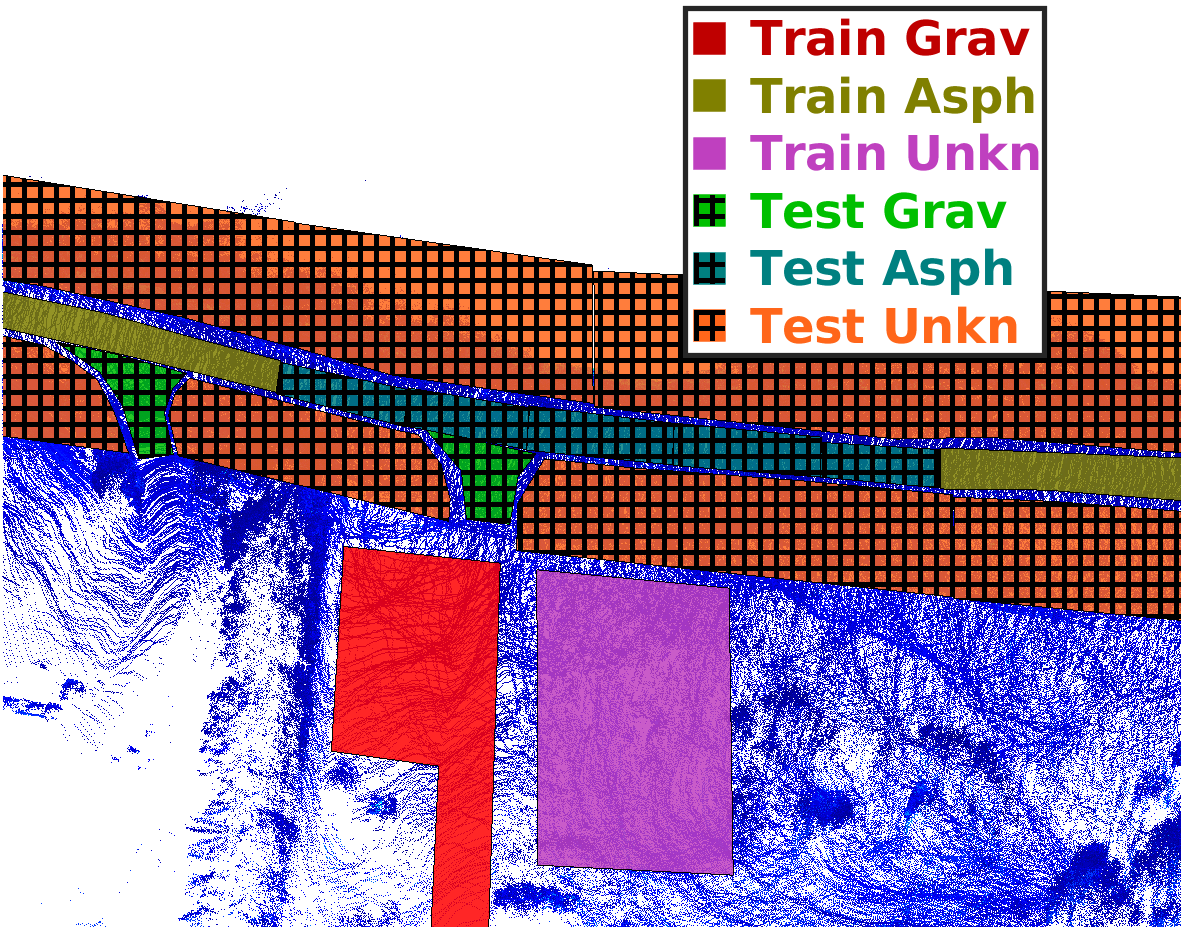
\includegraphics[width=0.95\linewidth]{Defense_Images/test_vs_train_areas_hatch}
			\caption[Training vs Testing Areas]{Training areas were kept separate from the testing areas.}
			\label{fig:test_vs_train_areas_in_results}
		\end{figure}
		
		% what does the manually defined areas look like?
		
		
	}
	
	

	\section{Training Data Extraction and Examination}\label{sec:training_data_extraction}{
		
		\begin{figure}[H]
			\centering
			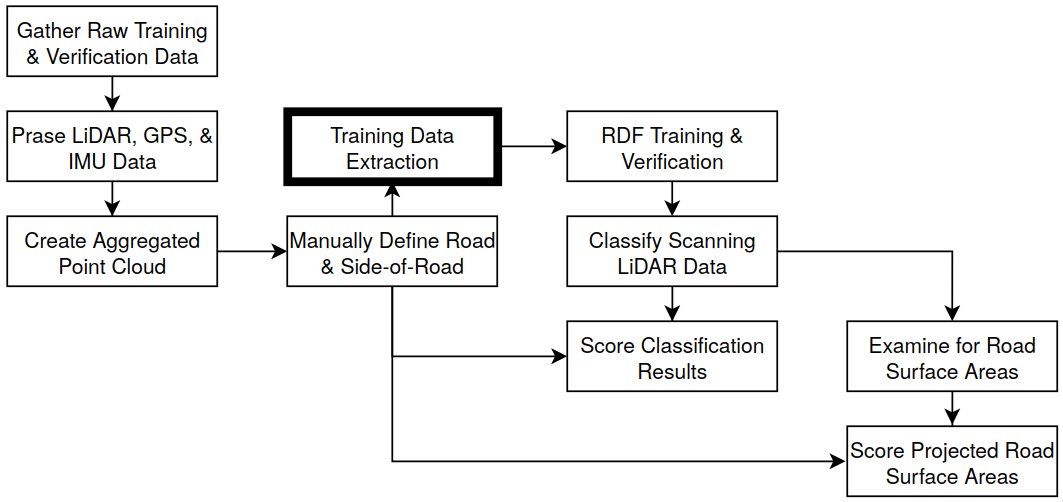
\includegraphics[width=0.9\linewidth]{Defense_Images/flowz_train_data_extract}
			\caption[Training Data Extraction Flowchart Context]{The following section addresses the process of extracting training data from manually defined areas.}
			\label{fig:flowz_train_data_extract}
		\end{figure}
		
		{Training data was extracted from an arc from the first three channels of scanning LiDAR data if coincident to manually defined areas. Arcs were defined by setting minimum and maximum angle boundaries and grabbing all LiDAR points from each channel that fell within the two boundaries. MATLAB's $inpolygon$ function was used to grab all points within the area. If 90\% of a single arc was inside the manually defined area, features were extracted from the arc. Features extracted are described in the Methodology section \ref{sec:Feat_Extract}.} 
		
		\begin{figure}[H]
			\centering
			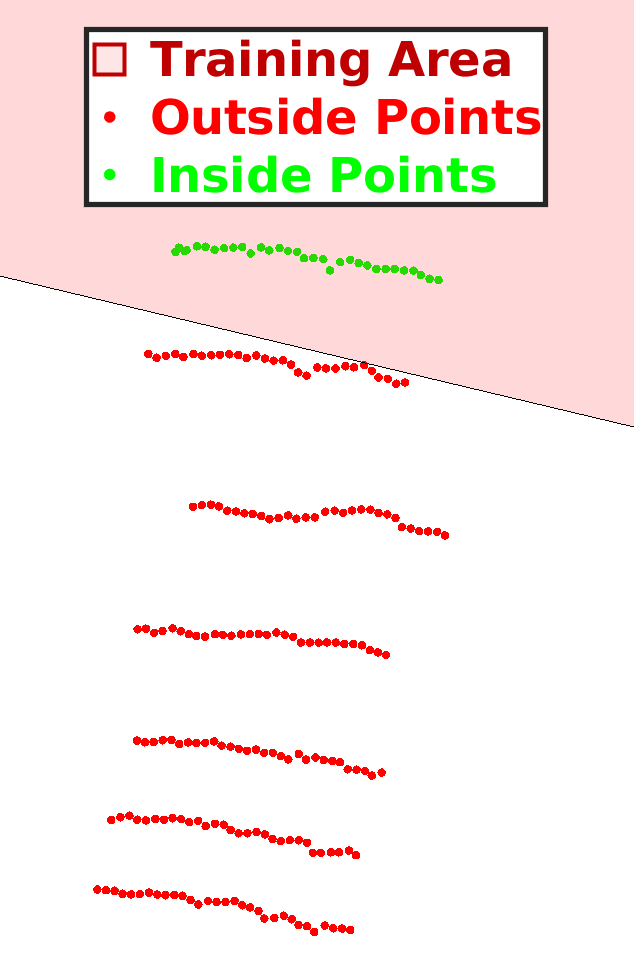
\includegraphics[width=0.5\linewidth]{Defense_Images/arc_in_mca_or_not}
			\caption[Coincident Point Example]{Each arc was examined to determine if the majority of it's points was within a manually defined area. This example shows arcs from a single channel as the experimental apparatus moves forward. Points that fall inside the manually defined training area were extracted to a database. }
			\label{fig:arc_in_mca_or_not}
		\end{figure}
		
		{Proper training of a machine learning algorithm dictates that equal numbers of training samples from each class in order that the algorithm does not over-classify testing and verification data as the majority class. Training data was examined to determine the class with the fewest number of samples. All samples from the class with the minimum samples was set aside, and an equal number of samples from the other two classes were randomly selected. Upon compiling the equalized training data, thirty percent was randomly selected and reserved for a validation data set.}
		
		{Training data was examined for clustering by comparing two feature sets against each other (Figure \ref{fig:range_training_data_cluster_3}, \ref{fig:ransac_training_data_cluster}, \ref{fig:mls_training_data_cluster}). It was found that MLS and RANSAC features were extremely similar, indicating that terrain classification results will be similar as well. Histograms were also used to visualize data feature clustering (Figure \ref{fig:ransac_two_histograms}). Low overlap in feature regions, called clustering, indicates that the classes are distinct from each other. High overlap in feature regions indicates that terrain types are not distinct from each other, as in the case of the dirt on the side of the Blackburn Road (Figure \ref{fig:dirt_v_gravel2}). }
		
		\begin{figure}[H]
			\centering
			\includegraphics[width=0.65\linewidth]{Defense_Images/ransac_training_data_cluster}
			\caption[Example RANSAC Clustering]{Example of training data generated with a RANSAC projected plane reference point features compared.}
			\label{fig:ransac_training_data_cluster}
		\end{figure}
	
		\begin{figure}[H]
			\centering
			\includegraphics[width=0.65\linewidth]{Defense_Images/mls_training_data_cluster}
			\caption[Example MLS Clustering]{Example of training data generated with a MLS projected plane reference point features compared.}
			\label{fig:mls_training_data_cluster}
		\end{figure}
	
		\begin{figure}[H]
			\centering
			\begin{subfigure}{0.45\textwidth}
				\centering
				\includegraphics[width=1.0\linewidth]{Defense_Images/Ransac_Histogram_example_1}
				\caption[Feature Histogram Example 1]{}
				\label{fig:Ransac_Histogram_example_1}
			\end{subfigure}
			\begin{subfigure}{0.45\textwidth}
				\centering
				\includegraphics[width=1.0\linewidth]{Defense_Images/Ransac_Histogram_example_2}
				\caption[Feature Histogram Example 2]{}
				\label{fig:Ransac_Histogram_example_2}
			\end{subfigure}
			\caption[Feature Histograms]{Histograms were also used to help visualize data features to ensure trainability of a machine learning algorithm.}
			\label{fig:ransac_two_histograms}
		\end{figure}
		
		\begin{figure}[H]
			\centering
			\includegraphics[width=0.65\linewidth]{Defense_Images/dirt_v_gravel2}
			\caption[Dirt vs Gravel]{Dirt being re-grassed leads to terrain classification confusion with gravel surfaces due to an overlap in extracted features. }
			\label{fig:dirt_v_gravel2}
		\end{figure}
		
	} % Training Data Extract
		
	
	\section{Random Decision Forest Training and Verification}\label{sec:rdf_train_verify}{
		
		\begin{figure}[H]
			\centering
			\includegraphics[width=0.9\linewidth]{Defense_Images/flowz_rdf_train}
			\caption[RDF Training Flowchart Context]{The following section addresses the process of training random decision forests.}
			\label{fig:flowz_rdf_train}
		\end{figure}
		
		{MATLAB was used to train Random Decision Forest terrain classification algorithms using the Classifier Learner App (Figure \ref{fig:classifier_app}). Training data was loaded into the application. Validation methods for the trained model include Hold-out Validation, Cross Validation, and Resubstitution Validation. Resubstitution Validation, the chosen option, uses all the training data for training and initial validation (Section \ref{sec:Feat_Extract}). Decision tree depth, number of learners (bagged decision trees), and number of features to consider for each binary split are hyper-parameters that were optimized using MATLAB's Bayesian Optimization. Bayesian Optimization automates the manual hyper-parameter tuning process by creating a surrogate model representing the objective function, in this case out-of-bag error (Figure \ref{fig:c2_min_class_error}, \ref{fig:c2_min_class_error_ransac}, \ref{fig:c2_min_class_error_mls}). Testing for over-fitting was accomplished by comparing out-of-bag training error to validation error (Figure \ref{fig:train_vs_valid_overfit_test2}, \ref{fig:train_vs_vali_ransac}, \ref{fig:train_vs_vali_mls}). Confusion matrices provide insight to algorithm capability of accurately classifying the validation data set by comparing  actual and predicted classes (Figure \ref{fig:vali_err_conf_mat_range} \ref{fig:c2_vali_conf_ransac} \ref{fig:c2_vali_confmat_mls}).} 
		
		\begin{figure}[H]
			\centering
			\includegraphics[width=0.9\linewidth]{Defense_Images/classifier_app_2}
			\caption[Classifier App]{MATLAB's Classifier App was used to train Random Decision Forests using Bayesian Optimization. }
			\label{fig:classifier_app}
		\end{figure}
		
		\begin{figure}[H]
			\centering
			\begin{subfigure}{0.45\textwidth}
				\centering
				\includegraphics[width=1.0\linewidth]{Defense_Images/c2_bayesian_ransac}
				\caption[Bayesian Optimization - RANSAC]{}
				\label{fig:c2_min_class_error_ransac}
			\end{subfigure}
			\begin{subfigure}{0.45\textwidth}
				\centering
				\includegraphics[width=1.0\linewidth]{Defense_Images/c2_bayesian_mls}
				\caption[Bayesian Optimization - MLS]{}
				\label{fig:c2_min_class_error_mls}
			\end{subfigure}
			\caption[Bayesian Optimization - RANSAC/MLS]{Classification error during Bayesian Optimization tuning with RANSAC (a) and MLS (b) to project a reference plane for generating spatial features.}
			\label{fig:c2_min_class_error_ransac_mls}
		\end{figure}
		
		\begin{figure}[H]
			\centering
			\begin{subfigure}{0.45\textwidth}
				\centering
				\includegraphics[width=1.0\linewidth]{Defense_Images/train_vs_vali_ransac}
				\caption[Training vs Validation Error - RANSAC]{}
				\label{fig:train_vs_vali_ransac}
			\end{subfigure}
			\begin{subfigure}{0.45\textwidth}
				\centering
				\includegraphics[width=1.0\linewidth]{Defense_Images/train_vs_vali_mls}
				\caption[Training vs Validation Error - RANSAC]{}
				\label{fig:train_vs_vali_mls}
			\end{subfigure}
			\caption[Training vs Validation Error - RANSAC/MLS]{Out of bag training versus validation error with RANSAC (a) and MLS (b) to project the reference plane for generating spatial features. }
			\label{fig:train_vs_vali_ransac_mls}
		\end{figure}
		
		\begin{figure}[H]
			\centering
			\begin{subfigure}{0.45\textwidth}
				\centering
				\includegraphics[width=1.0\linewidth]{Defense_Images/c2_vali_conf_ransac}
				\caption[Validation Confusion Matrices - RANSAC]{}
				\label{fig:c2_vali_conf_ransac}
			\end{subfigure}
			\begin{subfigure}{0.45\textwidth}
				\centering
				\includegraphics[width=1.0\linewidth]{Defense_Images/c2_vali_confmat_mls}
				\caption[Validation Confusion Matrices - MLS]{}
				\label{fig:c2_vali_confmat_mls}
			\end{subfigure}
			\caption[Validation Confusion Matrices - RANSAC/MLS]{Confusion matrices provide visual representation on the validation dataset classification accuracy.}
			\label{fig:vali_confmat_ransac_mls}
		\end{figure}
		
	} %rdf_train_verify
		
	\section{Classifying Consecutive Scanning LiDAR}\label{sec:classify_consec_scan_lidar}{
		
		\begin{figure}[H]
			\centering
			\includegraphics[width=0.95\linewidth]{Defense_Images/test_2.png}
			\caption[Classifying Consecutive LiDAR Scans Flowchart Context]{The following section addresses the process classifying consecutive LiDAR scans.}
			\label{fig:test_2.png}
		\end{figure}
			
		{Classifying consecutive LiDAR scans was accomplished by examination of the nine arcs of interest in front and forty-five degree angles left and right from the front of the experimental apparatus (Fig. \ref{fig:area_example}). Features from each arc were extracted and the arc was classified (Figure \ref{fig:range_raw_results_example}). Classification of real-world data outside of the training data set presents difficulties to the generated Random Decision Forest Classifiers generated in this work. Due to the side of the road was being re-grassed near a portion of the asphalt road, the terrain classification algorithm struggled to differentiate the dirt from gravel, leading to some miss-classification of the side-of-road areas. Examination of the feature distribution shows a high amount of overlap (Fig. \ref{fig:dirt_v_gravel2}). Training a terrain classification algorithm to re-classify any gravel classification as either "unknown" or "gravel" was explored. Training data from the dirt area was gathered as in the method described in Section \ref{sec:training-data-collection} and used to train an RDF in the method described in Section \ref{sec:rdf_train_verify}. Exploitation of confidence scores to adjust results by requiring a very high confidence for positive gravel surface classification was explored. Confidence scores were examined to determine if road surfaces may be more easily discovered by eliminating data based on a threshold (Figure \ref{fig:conf_results}). }
		
		% RANGE
		\begin{figure}[H]
			\centering
			\begin{subfigure}[b]{\textwidth}
				\centering
				\includegraphics[width=0.9\textwidth]{Defense_Images/db_4_raw_range}
				\caption{}
				\label{fig:db_4_raw_range}
			\end{subfigure}
			\vspace{1cm} % Adjust the vertical space between the subfigures
			\begin{subfigure}[b]{\textwidth}
				\centering
				\includegraphics[width=0.9\textwidth]{Defense_Images/db_6_raw_range}
				\caption{}
				\label{fig:db_6_raw_range}
			\end{subfigure}
			\caption[Raw Result Example - RANGE Spatial Reference Point]{Two examples of raw classification results using an algorithm that used the range from LiDAR point of origin as the spatial reference point. }
			\label{fig:range_raw_results_example}
		\end{figure}
		

		\begin{figure}[H]
			\centering
			\begin{subfigure}[b]{\textwidth}
				\centering
				\includegraphics[width=0.9\textwidth]{Defense_Images/range_db_4_conf_size_example}
				\caption{}
				\label{fig:range_db_4_conf_size_example}
			\end{subfigure}
			\vspace{1cm} % Adjust the vertical space between the subfigures
			\begin{subfigure}[b]{\textwidth}
				\centering
				\includegraphics[width=0.9\textwidth]{Defense_Images/range_db_4_conf_trim_example}
				\caption{}
				\label{fig:range_db_4_conf_trim_example}
			\end{subfigure}
			\caption[]{Classification confidence scores were examined to determine if road surfaces may be more easily discovered. Increased confidence results in a larger marker size (a). Classification results with a confidence level below a threshold was eliminated (b).}
			\label{fig:conf_results}
		\end{figure}
		
	} % Classifying Consecutive Scanning LiDAR
	
	
	\section{Consecutive Scanning LiDAR Classification Scoring}\label{sec:consec_class_scoring}{
		
		{Manually defined areas were derived using the process described in \ref{sec:training_and_verification_data_selection_process}. Gravel, asphalt, and side-of-road truth areas were projected onto the classified point cloud for the determination of classification accuracy. Averaged x, y, and z coordinates were taken of each arc and projected unto a manually defined truth area map (Fig. \ref{fig:rm_db_4_toc}). Distribution of classified points per area was determined and used to calculate per-area score. Per-area scores were averaged over the five drive-bys and tabulated (Table \ref{tab:average_per_area_score_results}). Process was completed for each of the three algorithm sets considered. It was found that the \textbf{RANGE}\footnotemark algorithm obtained a average true-positive accuracy of all intercepting gravel surfaces was 67.54\% (Fig. \ref{fig:range_example_area_score}). It was found that an average true-positive accuracy of all asphalt surfaces was 78.06\%. Differentiation between gravel road surfaces and surrounding terrain is necessary to determine boundaries for trajectory tracking and navigation. Overall average distribution for "unknown" terrain class within side-of-road areas was found to be 77.94\%. Other algorithms performed similarly to each other in terms of gravel and asphalt true-positive classification rate, however there \textbf{RANGE} exhibits a substantial increase when detecting side-of-road areas. For this reason, the \textbf{RANGE} algorithm was chosen as the best performing algorithm.}
		
		\footnotetext[1]{See Section \ref{sec:Feat_Extract} for definitions. } 
	
		\begin{table}[H]
			\centering
			\begin{tabular}{c|c|c|c|}
																	& Areas        & Distribution \% 		& Median \% 	\\[-4pt]
				\hline
				\multirow{3}{*}{\rotatebox{90}{\textbf{RANGE}}}  	& Gravel       & 69.15   				& 68.98    		\\[-4pt]
																	& Asphalt      & 78.07   				& 78.07    		\\[-4pt]
																	& Side of Road & 77.64   				& 79.94    		\\[-4pt]
				\hline
				\multirow{3}{*}{\rotatebox{90}{\textbf{RANSAC}}} 	& Gravel       & 65.91   				& 74.74    		\\[-4pt]
																	& Asphalt      & 87.13   				& 78.70    		\\[-4pt]
																	& Side of Road & 60.66   				& 52.59    		\\[-4pt]
					\hline
				\multirow{3}{*}{\rotatebox{90}{\textbf{MLS}}}    	& Gravel       & 74.38   				& 87.13    		\\[-4pt]
																	& Asphalt      & 78.70   				& 87.13    		\\[-4pt]
																	& Side of Road & 53.69   				& 61.05    
			\end{tabular}
			\caption[Averaged Area Score Results]{Average per-area score results for the three considered algorithms.}
			\label{tab:average_per_area_score_results}
		\end{table}
		
		\begin{figure}[H]
			\centering
			\includegraphics[width=0.95\linewidth]{Defense_Images/range_actual_rm_db_4_area_score}
			\caption[Area Scores: RANGE]{Example of per-area score using the \textbf{RANGE} algorithm}
			\label{fig:range_example_area_score}
		\end{figure}
	
		\begin{figure}[H]
			\centering
			\includegraphics[width=0.95\linewidth]{Defense_Images/ransac_actual_db_4_area_score}
			\caption[Area Scores: RANSAC]{Example of per-area score using the \textbf{RANSAC} algorithm.}
			\label{fig:ransac_example_area_score}
		\end{figure}
	
		\begin{figure}[H]
			\centering
			\includegraphics[width=0.95\linewidth]{Defense_Images/mls_db_4_area_scores}
			\caption[Area Scores: MLS]{Example of per-area score using the \textbf{MLS} algorithm. Note the low Unknown score (27.82\%) in the lower right side-of-road area.}
			\label{fig:mls_example_area_score}
		\end{figure}
	
		{Including asphalt miss-classification in gravel areas for an overall road area detection score results in average true-positive road detection accuracy increasing to 79.18\% (\textbf{RANGE}, Table \ref{tab:adjusted_grav_avg_score}), a 10.02\% increase over raw results. Out of three instances of where the gravel class distribution was below 50\%, two gravel driveway areas saw an increase to greater than 50\%, indicating that asphalt classification inclusion may be beneficial to unmarked road detection at the expense of true-positive detection of road surface type.}
	
		\begin{table}[H]
			\centering
			\begin{tabular}{l|c}
									& Adjusted \% \\
				\hline
				\textbf{RANGE}  	& 79.18       \\[-4pt]
				\textbf{RANSAC} 	& 78.94       \\[-4pt]
				\textbf{MLS}    	& 72.63      
			\end{tabular}
			\caption[Adjusted Averaged Gravel Area Score]{If asphalt and gravel classification distributions are combined for an overall road area detection within gravel areas, a slight increase over raw gravel distribution is found. Increased score over raw gravel results may indicate a benefit to differentiating general road area vs non-road areas.}
			\label{tab:adjusted_grav_avg_score}
		\end{table}

		{Confusion between dirt and gravel (Section \ref{sec:training-data-collection} \ref{sec:classify_consec_scan_lidar}) usually results in poor side-of-road detection (see \ref{fig:mls_example_area_score}). Implementation of a dedicated algorithm to further test terrain classified as gravel was explored by training an algorithm with gravel and dirt training data. As the closest channel was the most effected by the confusion, the closest channel was re-examined initially for proof of concept. Although the true side-of-road detection rate (Figure \ref{fig:dvg_example}) did improve (15.38\% increase in side-of-road detection), it came with increased false-negatives in gravel terrain discovery in addition to increased computational load. Original results (Figure \ref{fig:db_4_raw_range_2}) show side of road areas having a distribution majority of unknown classifications, indicating that the additional classification algorithm may not be needed to detect side-of-road areas.} 
		
%		dvg_example
		% RANGE
		\begin{figure}[H]
			\centering
			\begin{subfigure}[b]{\textwidth}
				\centering
				\includegraphics[width=0.9\textwidth]{Defense_Images/range_actual_rm_db_4_area_score}
				\caption{}
				\label{fig:db_4_raw_range_2}
			\end{subfigure}
			\vspace{1cm} % Adjust the vertical space between the subfigures
			\begin{subfigure}[b]{\textwidth}
				\centering
				\includegraphics[width=0.9\textwidth]{Defense_Images/dvg_example}
				\caption{}
				\label{fig:dvg_example}
			\end{subfigure}
			\caption[Complementary RDF Area Scores]{\textbf{RANGE} was supplemented with an algorithm that re-examined gravel classifications to determine if the correct classification was dirt. Results indicate that this method did improve side-of-road detection rate at the expense of lowered gravel detection rate. }
			\label{fig:area_score_comp}
		\end{figure}
	
		{Random Decision Forests were trained for all nine arcs individually (\textbf{RANGELCR} in Table \ref{tab:dvg_result_table}) to determine if an increase in accuracy over a per-channel algorithm could be obtained. While the same procedure was followed as described to train, verify, and test the algorithms, it was found that the RDFs struggled to differentiate between road and non-road terrain while offering little benefit in true positive gravel or asphalt identification. As the per-channel \textbf{RANGE} algorithm performed well enough for this work in terms of demonstrating method feasibility, \textbf{RANGELCR} was subsequently dropped. Future work may be done to analyze the per-arc RDF training process to better understand why a lower accuracy was found and implement a better solution.}
		
		\begin{table}[H]
			\centering
			\begin{tabular}{c|c|c|c|}
																	& Areas        & Distribution \% 		& Median \% 	\\[-4pt]
				\hline
				\multirow{3}{*}{\rotatebox{90}{\textbf{RANGE}}}  	
																	& Gravel       & 69.15   				& 68.98    		\\[-4pt]
																	& Asphalt      & 78.07   				& 78.07    		\\[-4pt]
																	& Side of Road & 77.64   				& 79.94    		\\[-4pt]
				\hline
				\multirow{3}{*}{\rotatebox{90}{\textbf{RANGELCR}}} 	
																	& Gravel       & 68.03   				& 71.06    		\\[-4pt]
																	& Asphalt      & 78.02   				& 83.01    		\\[-4pt]
																	& Side of Road & 49.97 					& 45.86 
			\end{tabular}
			\caption[RANGE vs RANGELCR]{Individual RDFs were trained for each considered arc. Average scores were compared. }
			\label{tab:dvg_result_table}
		\end{table}
		
		
	}
	
	
	\section{Visual Detection of Unmarked Road Surfaces}\label{sec:vis_det}{
		
		{Classified point clouds were manually examined for 'best guess' locations for gravel and asphalt surfaces. Two out of three positive gravel identifications must be made on each channel, be evenly spaced, and be relatively co-planar to other road surface guesses in order for a positive guess for an asphalt or gravel surface to be made (Figures \ref{fig:range_example_vis_score} \ref{fig:ransac_example_vis_score} \ref{fig:mls_example_vis_score}). Guessed areas that partially overlayed truth areas were given a score of 0.5, while guessed areas that fully overlayed truth areas were given a score of 1. Driveways $1$ and $2$ were detected in all five drive-bys and $3$ was detected in four of the five, leading to an 89.17\% accuracy in intercepting gravel road detection using the \textbf{RANGE} algorithm (Table \ref{tab:road_area_overlap_score}). It was found that in three drive-bys there was a false positive driveway detection, however the location of the false-positives were not repeated in any of the other drive-bys. In all drive-bys the asphalt road was consistently visually detected, however there were gravel areas that were consistently found in front of the gravel areas (Figure \ref{fig:gravel_on_asphalt}). Out of all drivebys using \textbf{RANGE}, only a single asphalt area contained less than a 50\% distribution of asphalt areas, all others being at or near 100\% asphalt, indicating the algorithm is sufficient at detecting unmarked asphalt roads. True-positive gravel road detection rates using \textbf{MLS} and \textbf{RANSAC} were similar and significantly lower than that of \textbf{RANGE} while also having a similar and significantly higher false-positive gravel road detection rate (Table \ref{tab:road_area_overlap_score}). Due to the similar performances between \textbf{RANSAC} and \textbf{MLS} in both visual detection unmarked road identification as well as per-area distribution scores (Section \ref{sec:consec_class_scoring}), it is indicated that using a projected plane on as a reference point may not be beneficial to terrain classification.}
		
		\begin{figure}[H]
			\centering
			\includegraphics[width=0.95\linewidth]{Defense_Images/pre_guess}
			\caption[Visual Scores: RANGE Source]{Close-up of example classified point cloud that has a trend of road surface classes across three channels. Road surface areas were then guessed and projected onto the classified results (Figure \ref{fig:range_example_vis_score}).}
			\label{fig:pre_guess}
		\end{figure}
		
		\begin{figure}[H]
			\centering
			\includegraphics[width=0.95\linewidth]{Defense_Images/range_db_6_overlap_2}
			\caption[Visual Scores: RANGE]{Example of visual road surface detection using the \textbf{RANGE} algorithm showing gravel driveway $3$ being visually detected.}
			\label{fig:range_example_vis_score}
		\end{figure}
		
		\begin{figure}[H]
			\centering
			\includegraphics[width=0.5\linewidth]{Defense_Images/ransac_db_6_overlap_2}
			\caption[Visual Scores: RANSAC]{Example of visual road surface detection using the \textbf{RANSAC} algorithm showing gravel driveway $3$ being visually detected.}
			\label{fig:ransac_example_vis_score}
		\end{figure}
		
		\begin{figure}[H]
			\centering
			\includegraphics[width=0.5\linewidth]{Defense_Images/mls_db_6_overlap_2}
			\caption[Visual Scores: MLS]{Example of visual road surface detection using the \textbf{MLS} algorithm showing gravel driveway $3$ being visually detected.}
			\label{fig:mls_example_vis_score}
		\end{figure}
		
		\begin{table}[H]
			\centering
			\begin{tabular}{l|c|c}
									& Grav Road Det. \% 	& Avg Grav False Pos\footnotemark	\\
				\hline
				\textbf{RANGE}  	& 89.17       			& 0.60	\\[-4pt]
				\textbf{RANSAC} 	& 56.67       			& 2.40	\\[-4pt]
				\textbf{MLS}    	& 76.67 				& 2.60		
			\end{tabular}
			\caption[Road Area Detection Score]{Gravel and Asphalt road detection scores. Average number of gravel road false-positives per drive-by were found.}
			\label{tab:road_area_overlap_score}
		\end{table}
		\footnotetext[1]{In all drive bys there were no false detection of asphalt surface areas.}
	
		\begin{figure}[H]
			\centering
			\includegraphics[width=0.95\linewidth]{Defense_Images/gravel_on_asphalt}
			\caption[Gravel on Asphalt]{Gravel on asphalt areas (red) consistently resulted in gravel classification.}
			\label{fig:gravel_on_asphalt}
		\end{figure}
		
	
	}
	
	\section{Automated Detection of Unmarked Road Surfaces}\label{sec:auto_det}{
		
		
		{Automated detection of unmarked road was explored in a post-processing step in order to determine if visual detection results may be repeated. \textbf{RANGE} results were analyzed, as this algorithm provided the best results (Section \ref{sec:consecutive_point_cloud_classification_scoring}). Center, left, and right areas were used to isolate per-channel classification results (Figure \ref{fig:auto_guess_areas}). Trends across classified arcs were exploited to determine the best guess at area terrain type. Guessed areas were aggregated into a larger map then compared to truth areas (Figure \ref{fig:agreggated_auto_guess}). It was found that while the true-positive gravel road rate lessened with 89.17\% vs 70.00\% for visual and automated road surface detection respectively (Figure \ref{fig:guess_grav_intersect}), the number of false positives was much higher with 0.6 vs 1.0 average number of false positives per drive-by. This is partially due to the simplicity of the automated guessing method and the over-reliance on the raw classification results (Figure \ref{fig:6range_guess_unkn_misclass}). Most false-positives were a result of the RDF incorrectly classifying the terrain shown in Figure \ref{fig:here_be_side_of_road_dirt2} as gravel. Visual identification of unmarked road surfaces used spatial distribution of classification results that was not perfectly replicated in the automated plotting algorithm. Further work may be done in the future to lower the rate of false-positives, however, current work suffices as proof of concept. Rate of processing classified results took under one second, making real-time implementation of a similar model a future possibility. }
		
		\begin{figure}[H]
			\centering
			\includegraphics[width=0.95\linewidth]{Defense_Images/agreggated_auto_guess}
			\caption[Aggregated Automated Road Surface Detection]{Results from automated road detection were aggregated.}
			\label{fig:agreggated_auto_guess}
		\end{figure}
		
		\begin{figure}[H]
			\centering
			\includegraphics[width=0.95\linewidth]{Defense_Images/guess_grav_intersect}
			\caption[Aggregated Automated Road Surface Detection]{Aggregated automated road surface detection was compared to truth areas. }
			\label{fig:guess_grav_intersect}
		\end{figure}
		
		\begin{figure}[H]
			\centering
			\includegraphics[width=0.95\linewidth]{Defense_Images/6range_guess_unkn_misclass}
			\caption[Automated Road Surface False Positive]{}
			\label{fig:6range_guess_unkn_misclass}
		\end{figure}
		
		\begin{figure}[H]
			\centering
			\includegraphics[width=0.95\linewidth]{Defense_Images/here_be_side_of_road_dirt2}
			\caption[Blackburn Road Side of Road]{}
			\label{fig:here_be_side_of_road_dirt2}
		\end{figure}
		
	}



	\section{Rate of Classification}{
		
		{Classification was completed using Ubuntu 18.04 and an AMD Ryzen 9 5900X 12 core 24 thread. Rate of classification for all nine areas of interest in a single scan (using \textbf{RANGE}) was found to be an average of 35.19 ms using a single core (Fig. \ref{fig:per_arc_classification_time}) or 316.68 ms per 360 degree scan (Fig. \ref{fig:per_scan_classification_rate}). Further optimization may increase this speed, however real-time classification is not a focus of this work. When utilizing all 24 cores during a rate of 13.19 ms per 360 scan is achieved. Extrapolation from distance traveled indicates that a hypothetical 71.39 feet per second or 48.68 miles per hour may be possible.}
		
		\begin{figure}[H]
			\centering
			\includegraphics[width=0.9\linewidth]{Defense_Images/per_arc_classification_time}
			\caption[Per-Arc Time]{Per-arc classification time}
			\label{fig:per_arc_classification_time}
		\end{figure}
		
		\begin{figure}[H]
			\centering
			\includegraphics[width=0.9\linewidth]{Defense_Images/per_scan_classification_rate}
			\caption[Per-Scan Time]{Per-scan classification time}
			\label{fig:per_scan_classification_rate}
		\end{figure}
		
	}
		
} % End Results


\chapter{Conclusion}{
	
	{The proposed work addresses the problem of road surface detection on unmarked gravel and chipseal roads. Current LiDAR and Camera based detection models are insufficient due to lack of distinct features typical of urban roads, such as painted line markings or curbs, or have excessive computational or storage requirements. The completed work balanced accuracy and efficiency by using less intensive analysis techniques of smaller point cloud data sets. The first objective was to determine a method of detecting an unmarked gravel road. The second objective was to evaluate performance of road detection along stretches of unmarked gravel and chipseal roads. The final deliverable of the completed work was a method of detecting physical unmarked gravel and chipseal roads by using a terrain classification approach to predicting road surface area. The impact of this work is that autonomous vehicles using LiDAR may be able to detect gravel road surfaces in real time, allowing autonomous operations on 1.5 million miles of previously undetected rural roads.}

}


%\appendix
%
%\chapter{Source Code}{
%	
%	\section{Additional Tables}{
%	
%	
%	
%	}
%	
%	\section{MATLAB Source Code}{
		
%			\lstinputlisting[style=Matlab-editor, basicstyle=\mlttfamily\scriptsize, caption={PCD STACK CLASSIFIER}]{PCD_STACK_CLASSIFIER_DEFENSE_THING.m}
%			\lstinputlisting[style=Matlab-editor, basicstyle=\mlttfamily\scriptsize, caption={Grabbing Transformation Matrix}]{get_tform.m}
%			\lstinputlisting[style=Matlab-editor, basicstyle=\mlttfamily\scriptsize, caption={Making Combined Point Cloud}]{make_combined_pcd.m}
%			\lstinputlisting[style=Matlab-editor, basicstyle=\mlttfamily\scriptsize, caption={Matching Timestamps}]{matchTimestamps.m}
%			\lstinputlisting[style=Matlab-editor, basicstyle=\mlttfamily\scriptsize, caption={Progress Bar}]{parfor_progress.m}	
		
% End Appendix Obj 1 T 2

%} % End Chapter - Appendix Source Code

%
%%% The \references command marks the point where the bibliography will
%%% be inserted.  In the example below, the BibTeX commands are
%%% inserted into the macro definition, but one could also manually
%%% enter the bibliography entries if desired.
%\references{
%  %ETD does not define a particular required bibliography style.
%  %They DO require entries to end in a period UNLESS they end in a URL
%  %or DOI AND that DOIs be set in the same font as everything else.
%  %I have modified the alphaurl style file, to conform to these requirements.
%  
  \bibliographystyle{ieeetr}  
  \bibliography{resources.bib} 
%}

%%\appendix           % Indicates the transition from chapters to appendices.  
                    % Subsequent 

%%\chapter{An Appendix}
%%\section{A Section in the Appendix}

\end{document}
